\chapter{Literature Review}
\label{chap:review}

\graphicspath{{Chapter2/figures/}}

\lettrine{F}{irst}, this chapter presents the core work in sensemaking and visualization. Then, it reviews the literature on analytic provenance with a focus on visualization of provenance data for supporting sensemaking. Finally, it summarizes visualization techniques of time-oriented and network data because these two data types are heavily involved in the research questions addressed in the thesis.

%\section{Sensemaking}
\emph{Sensemaking} reflects how we make sense of the world so that we can act in it~\cite{Snowden2005}. Sensemaking has been studied in many different contexts, most notably including information science~\cite{Dervin1983}, human-computer interaction~\cite{Russell1993}, organizational studies~\cite{Weick1995} and intelligence analysis~\cite{Pirolli2005,Klein2003}. In this section, we review the sensemaking research discussed in these contexts, with an emphasis on the last two sensemaking models that have been highly applied in visualization research. 

\subsection{Gap-Bridging Metaphor}
Dervin develops a sensemaking theory focusing on information seeking and use behaviors~\cite{Dervin1983}. It underlies the cognitive gap that individuals experience when attempting to make sense of observed data. \autoref{fig:lr-dervin} summarizes this \emph{gap-bridging} metaphor. The theory assumes that people moves through time-space in some particular context and situation. Sensemaking starts when they encounter a gap that needs to overcome such as something is unclear or confused. To bridge the gap, they may seek and use information from a variety of sources such as documents, media and other people. These sources are evaluated based on relevant attributes to assess their usefulness. 

\begin{figure}[!htb]
	\centering
	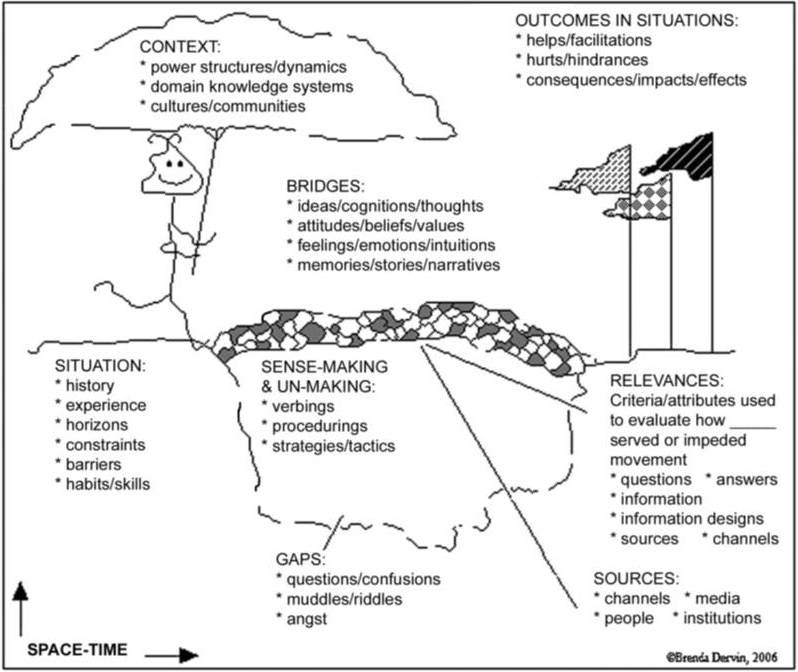
\includegraphics[width=\columnwidth]{dervin}
	\caption{The gap-bridging metaphor of sensemaking. People encounter gaps when moving through time-space, then seek for information, evaluate and use it to bridge the gaps. \is{Dervin2012}}
	\label{fig:lr-dervin}
\end{figure}

Dervin also implements the theory into a set of questions that can be used in interview to understand sensemaking within a context~\cite{Dervin1983}. The questions elaborate all parts of the model, aiming to establish an understanding on the situation (\emph{What happened?}), the gap (\emph{What did you struggle with?}), the bridge (\emph{What idea did you come to?}) and the outcome (\emph{How did that help?}).

\subsection{Learning Loop Complex}
In the context of human-computer interaction, Russell~et~al.~\cite{Russell1993} defines sensemaking as the process of searching for a representation and encoding data in that representation to answer task-specific questions. That cyclic process is called the \emph{learning loop complex} as illustrated in \autoref{fig:lr-russell}. First, the sensemaker searches for a representation to capture salient features of the data (\emph{Generation Loop}). During sensemaking, new information is sought and encoded into this representation (\emph{Data Coverage Loop}). The data unfit to the representation (\emph{residue}) requires the sensemaker to adjusts and produces a more suitable one. This entire learning loop complex is guided by the task with an aim to reduce its cost.

\begin{figure}[!htb]
	\centering
	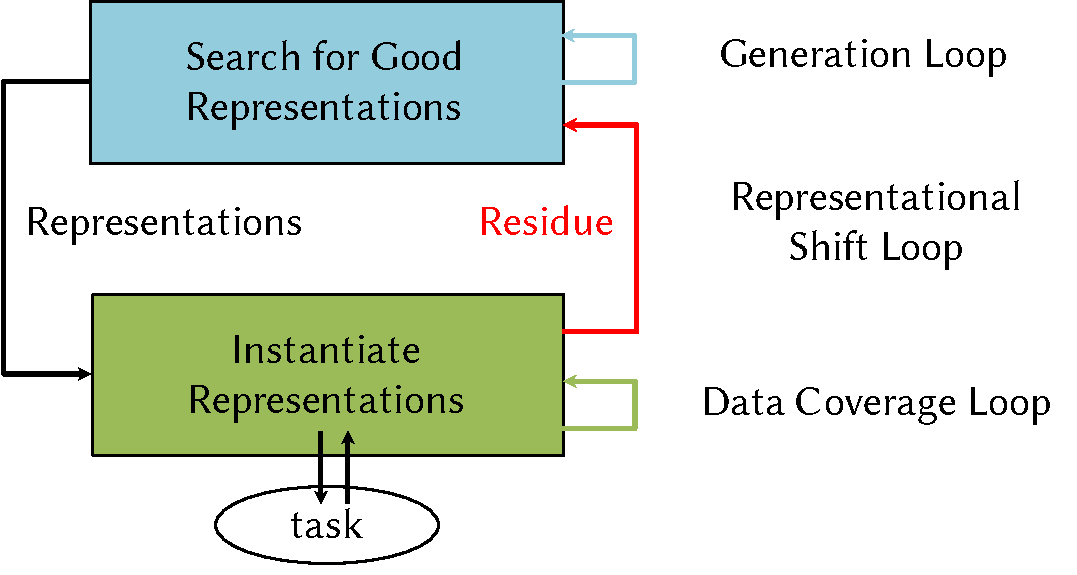
\includegraphics{russell}
	\caption{The learning loop complex theory of sensemaking. It consists of three iterative loops: searching for a good representation, encoding data to the representation, and adjusting the representation for a better data coverage. \is{Russell1993}}
	\label{fig:lr-russell}
\end{figure}

\subsection{Sensemaking in Organizations}
Different from Dervin and Russell who study sensemaking for individuals, Weick focuses on sensemaking at an organization level~\cite{Weick1995}. He proposes that sensemaking consists of these seven following properties.

\begin{enumerate}
	\item \emph{Grounded in identity construction}. Who people think they are, both individually and collectively, affect what they interpret and act.
	\item \emph{Retrospective}. People look back and make sense from what they have said and what they have done before.
	\item \emph{Enactive of sensible environments}. People make sense and contribute to the environments during their sensemaking processes.
	\item \emph{Social}. This is an inherent property of sensemaking in organization where people interact and socialize with others, and also are influenced by others.
	\item \emph{Ongoing}. Sensemaking is a continuous flow because the world and our understanding about the word are constantly changing.
	\item \emph{Focused on and by extracted cues}. Cues are things from the context that people have attention to and may use them to guide further exploration and assessment of the sensemaking problem.
	\item \emph{Driven by plausibility rather than accuracy}. Sensemaking is about plausibility and sufficiency rather than accuracy and completeness. People tend to stop searching when they find an acceptable solution.
\end{enumerate}

\subsection{A Process Model}
\label{sub:lr-pcm}
Pirolli and Card~\cite{Pirolli2005} describe sensemaking as an iterative process that gradually transforms raw data into rational knowledge. The process includes two sets of activities: one that cycles around finding relevant information, and another that cycles around making sense of that information, with plenty of interaction between them. They map to the \emph{foraging loop} and the \emph{sensemaking loop} respectively, as shown in \autoref{fig:lr-pirolli-card-model}. The sensemaking process can progress upward (from data to knowledge) or downward (from knowledge to data). The steps in the \emph{bottom-up} process are summarized as follows.

\begin{figure}[!htb]
	\centering
	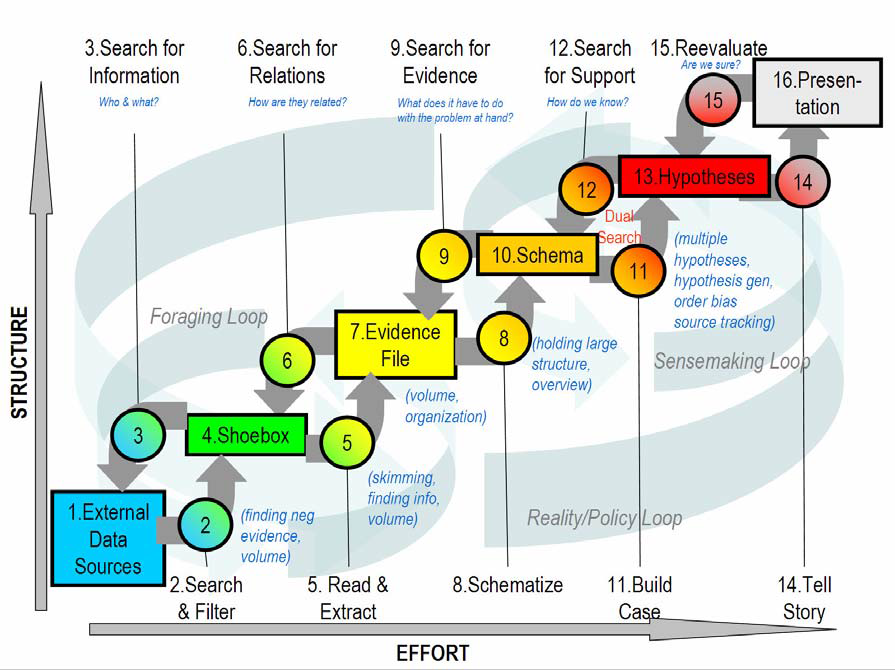
\includegraphics[width=\columnwidth]{pirolli-card-model}
	\caption{A notional model of sensemaking. The sub-processes (numbered circles) and their data input/output (numbered rectangles) are arranged in a two-dimensional space, in which the horizontal axis represents the degree of effort from users, and the vertical axis represents the degree of structure in information representation. \is{Pirolli2005}}
	\label{fig:lr-pirolli-card-model}
\end{figure}

\begin{itemize}
	\item \emph{Search and filter}. External data sources, such as classified databases or the web, are searched and filtered to retrieve relevant documents to the task.
	\item \emph{Read and extract}. These documents are examined to extract pieces of information that may be used as evidence later.
	\item \emph{Schematize}.  The collected information is organized in a way that aids the analysis. This may be executed in user mind, using paper and pen, or with a complex computer-based system.
	\item \emph{Build case}. Multiple hypotheses are generated; evidence are marshaled to support or disconfirm them.
	\item \emph{Tell story}. Discovered cases are presented to some audience.
\end{itemize}

In this model, \emph{schematization} plays an important role in converting raw evidence to rational explanations, bridging the foraging and sensemaking loops. A study by Kang, Görg and John Stasko~\cite{Kang2011} agrees with this observation. In their study, all the participants who performed the sensemaking task well spent considerable time and effort in organizing their collected information. Their organizational schemes were flexible: a \emph{timeline} of related events, a \emph{map} connecting locations that a person has been to, and a \emph{diagram} showing relationships among suspicious targets.

\subsection{Data--Frame Model}
\label{sub:lr-dfm}
Klein et al.~\cite{Klein2003} propose a sensemaking model that centers around \emph{data} and \emph{frame}. Data is the information that a person receives or searches for, and frame is the mental structure that organizes and explains the relationship of such data. For instance, a frame can be a \emph{story}, explaining the chronology of events and the causal relationships between
them; or a \emph{map}, showing where the events take place and the routes between them. Sensemaking is considered as a deliberate effort to understand an event, starting when a person realizes a gap of their current understanding of that event. Klein and his associates describe seven activities involved in sensemaking and are summarized in \autoref{fig:lr-data-frame-model}.

\begin{figure}[!htb]
	\centering
	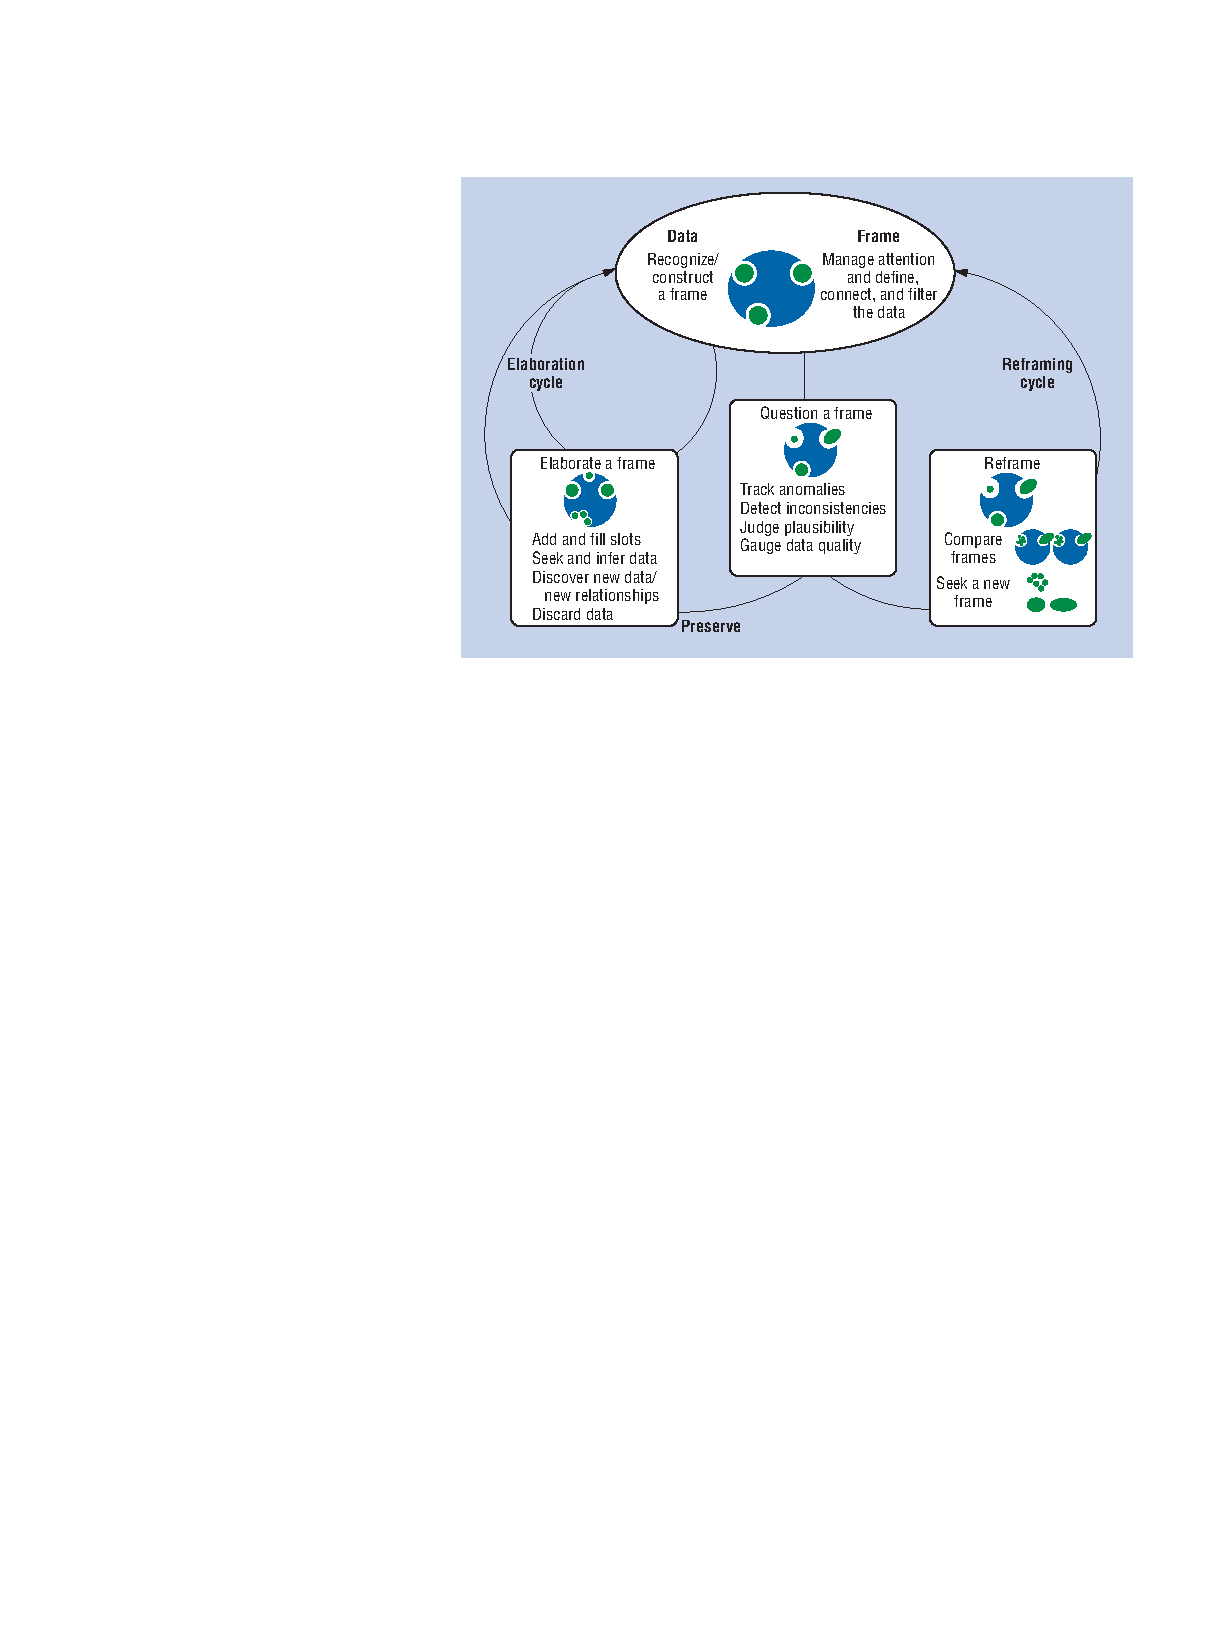
\includegraphics[width=\columnwidth]{data-frame-model}
	\caption{The data--frame model of sensemaking. It describes a set of interconnected sensemaking activities centering around data and frame -- the explanatory structure of data. \is{Klein2003}}
	\label{fig:lr-data-frame-model}
\end{figure}

\begin{itemize}
	\item \emph{Connect data and a frame}. A person recognizes relevant pieces of data and constructs an initial frame to explain them. The frame then helps the person to filter and search for new data.
	\item \emph{Elaborate the frame}. As more is learned about the situation, the frame becomes more elaborate with new data and new relationships. 
	\item \emph{Question the frame}. It happens when a person encounters data that is inconsistent with the existing frame. At this point, the person may be unsure that the frame is incorrect, or the inconsistent data is inaccurate.
	\item \emph{Preserve the frame}. A person may consider the severity of the inconsistent data, justify why it mismatches the frame, and ignore it.
	\item \emph{Compare multiple frames}. Depending on experience, a person may think of alternative frames explaining the same set of data. These frames need to be compared to select the most likely one.
	\item \emph{Reframe}. When encountering inconsistent and contrary data, the person may need to find a replacement that can explain all data. Considering discarded data and/or reinterpreting data could facilitate this activity.
	\item \emph{Seek a new frame}. A person may deliberately search for a new frame when encountering plenty of conflicted data. One or two key data elements may serve as \emph{anchors} to help the person to elicit another frame.
\end{itemize}

The Pirolli and Card's model describes a step-by-step process of sensemaking, in which the analyst collects relevant data and eventually transposes it into rational answers. However, the various sensemaking activities in the Data--Frame model may explain the strategies used by the analyst more comprehensively.

TODO: summary
A recent and comprehensive review of sensemaking can be found in the article by Maitlis and Christianson~\cite{Maitlis2014}.
%\section{Visualization and Visual Analytics}

\subsection{Overview}
Computer-based visualization systems provide visual representations of datasets designed to help people carry out tasks more effectively~\cite{Munzner2014}. Because the design space of possible visual ``idioms'' is huge, it is challenging to create effective visualizations. Understanding well-established information design principles and interaction techniques could guide designers toward the right direction. Also, every visualization needs to be evaluated to check whether it meets its design purposes and how it helps or hinder users.

Overview: what is vis? what can vis help? what is VA? what can VA help, in addition to vis? explain the VA process model. briefly explain the 3 important blocks in the model, which are then discussed in detail next. 

%What is vis? Classic example. What vis can help from cognition (Ben) and Wijk, Fekete?
%
%Large datasets -> simple aggregation, reduction like filtering, interaction, ; larger datasets, more sophiscated emthods extract patterns and vis to display them. and allow further. That is the idea of visual analytics. Orginal def, new def. Model.
%
%Describe visual analytics process model (Figure~\ref{fig:visual-analytics-process})
%
%\begin{figure}[!htb]
%	\centering
%	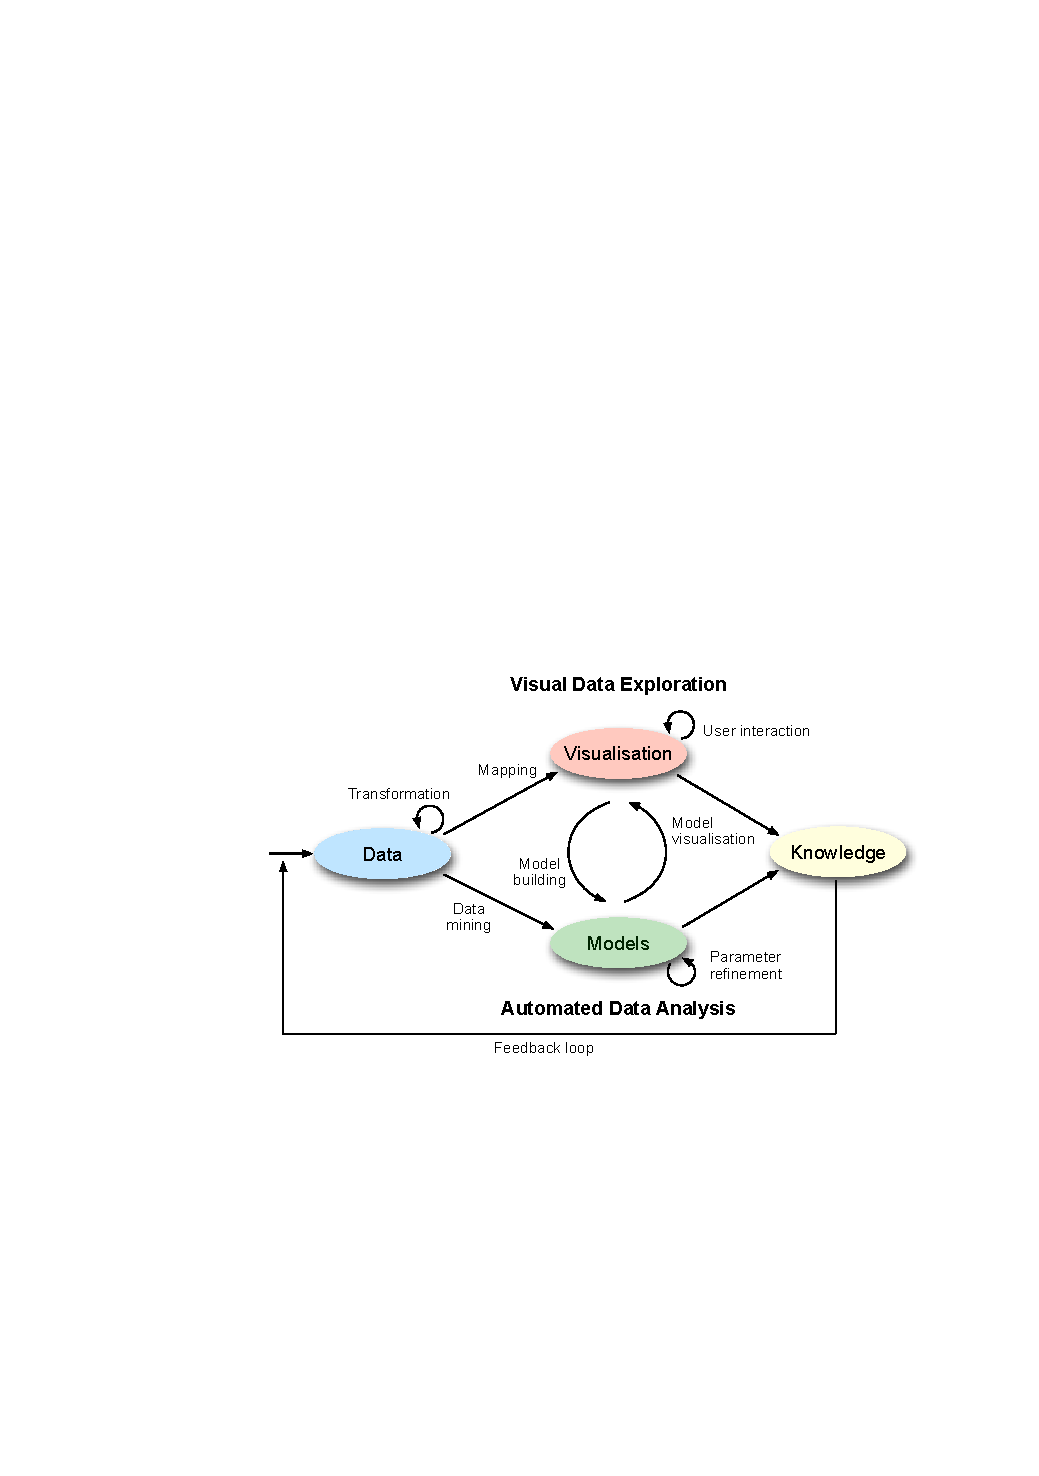
\includegraphics[width=\columnwidth]{visual-analytics-process}
%	\caption{The visual analytics process model. \emph{Source:~\cite{Keim2010}}.}
%	\label{fig:visual-analytics-process}
%\end{figure}
%
%
%Next, discuss basics of vis and models. and evaluation.

\subsection{Visualization Design}


\subsubsection{Information Design Principles}
\label{sub:lr-design}

\paragraph{Marks and Channels}
Marks are basic geometric elements that depict items or links, and channels control their appearance~\cite{Munzner2014}. Item marks can be zero-dimensional as a \emph{point}, one-dimensional as a \emph{line}, two-dimensional as an \emph{area}, and three-dimensional as a \emph{volume}, but rarely used. Link marks include \emph{connection} showing a pairwise relationship between two items using a line and \emph{containment} showing hierarchical relationships using areas. \autoref{fig:lr-marks} illustrates these marks. 

\begin{figure}[!htb]
	\centering
	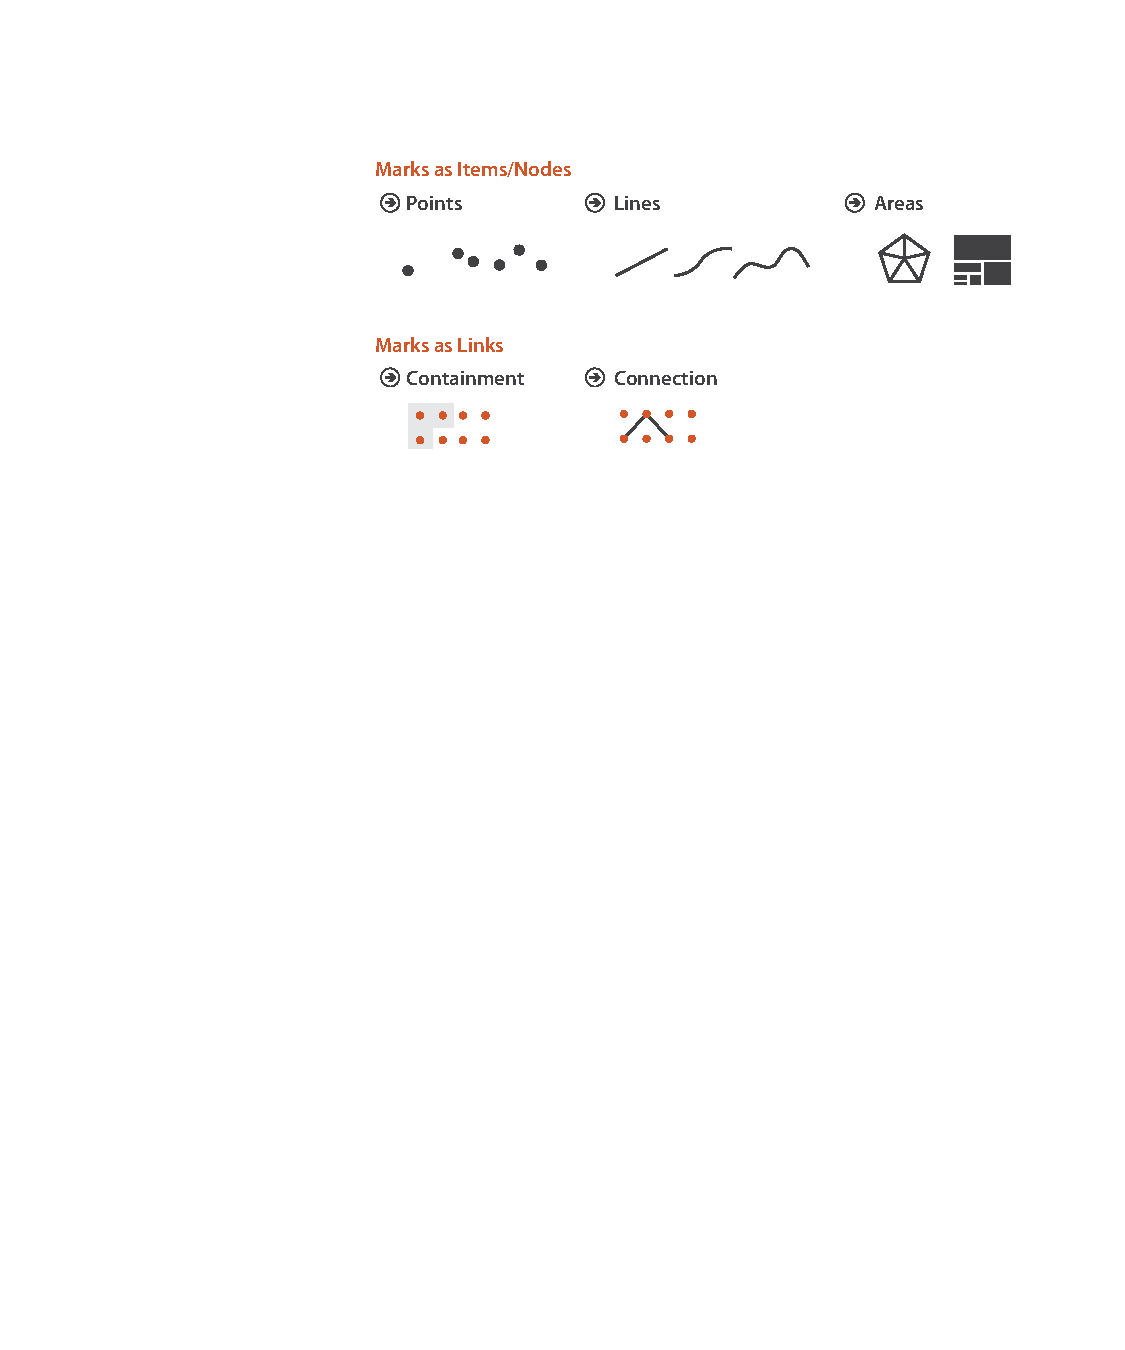
\includegraphics[width=.8\linewidth]{marks}
	\caption{Item and link marks as geometric primitives. \is{Munzner2014}}
	\label{fig:lr-marks}
\end{figure}

A visual channel control the appearance of marks, independent of their dimensionality. Examples include position, color, shape, angle and size. However, not all channels can be applied to all marks. For instance, an area mark is used in a geographic map to denote a region. It is already associated with a shape and size, thus cannot be size coded to represent another quantitative attribute.
some visual channels. some cannot encode size, example. \autoref{fig:lr-channel-example} shows a progression of chart types, with each showing one more data attribute using one more visual channel. \autoref{fig:lr-channel-example-1} shows a bar chart representing a single quantitative attribute using the \emph{vertical position} channel. \autoref{fig:lr-channel-example-2} shows a scatter plot encoding the second quantitative attribute using the \emph{horizontal position} channel. \autoref{fig:lr-channel-example-3} adds the \emph{color} channel to represent a categorical attribute, and \autoref{fig:lr-channel-example-4} adds the \emph{size} channel to represent another quantitative attribute. In these examples, each attribute is encoded with a single channel. However, multiple channels can be combined to redundantly encode the same attribute, helping perceive it more easily.

\begin{figure}[!htb]
\centering
\subcaptionbox{Line marks with horizontal position for a categorical attribute and vertical position for a quantitative attribute.\label{fig:lr-channel-example-1}}{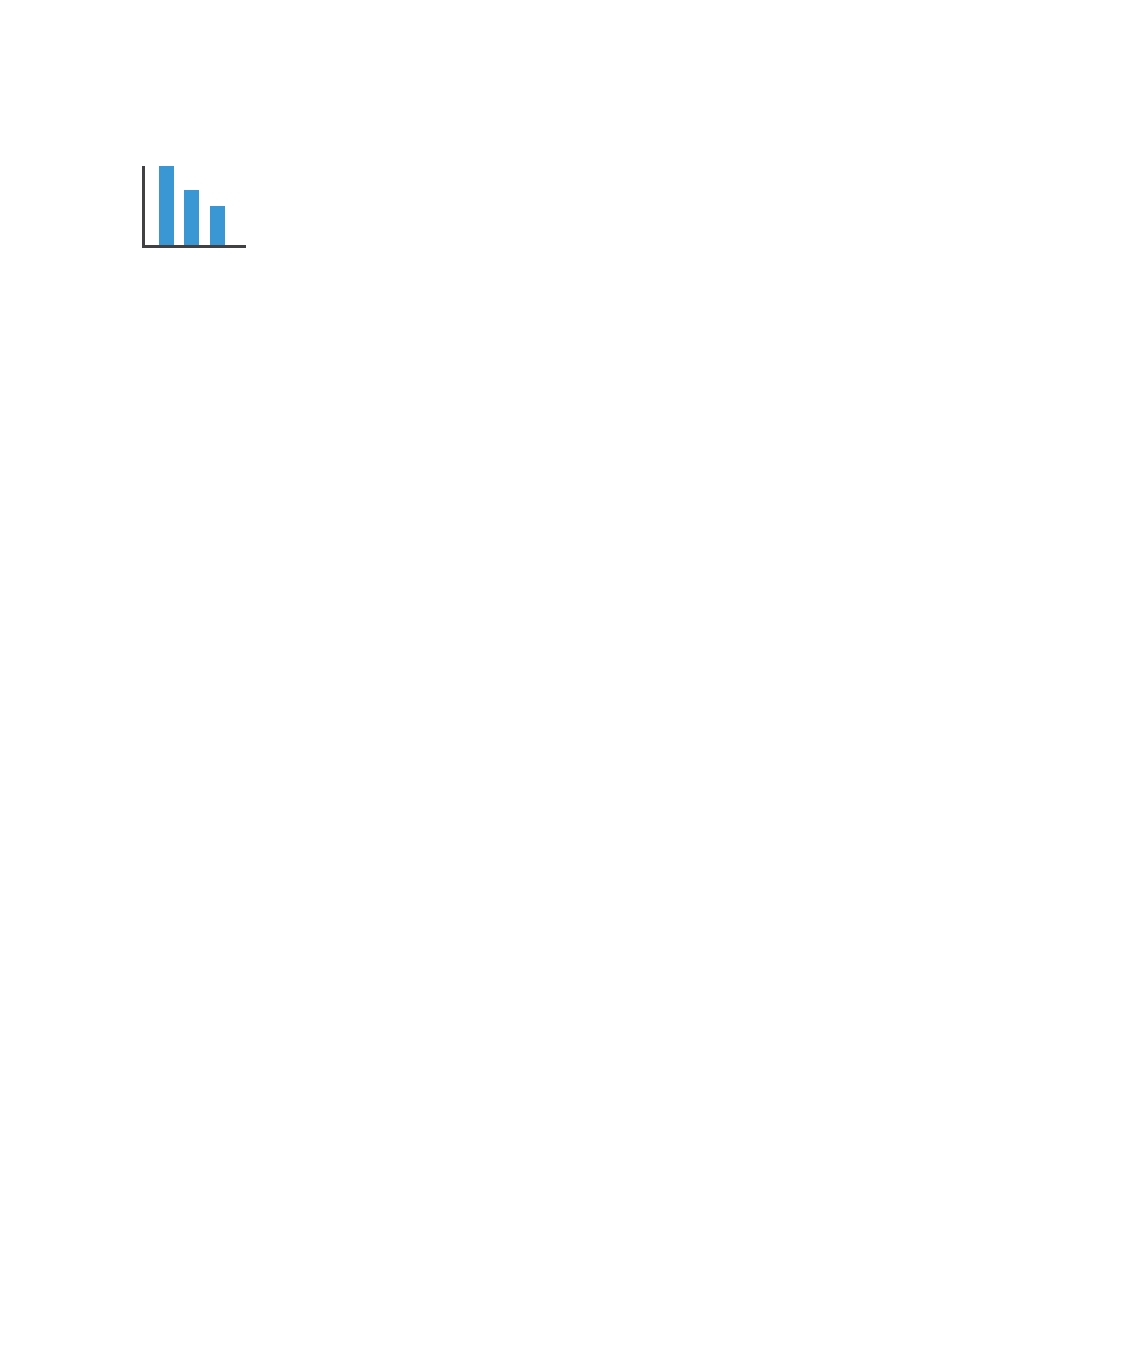
\includegraphics[width=.23\columnwidth]{channel-example-1}} 
\hfill
\subcaptionbox{Point marks with both horizontal and vertical position channels for quantitative attributes.\label{fig:lr-channel-example-2}}{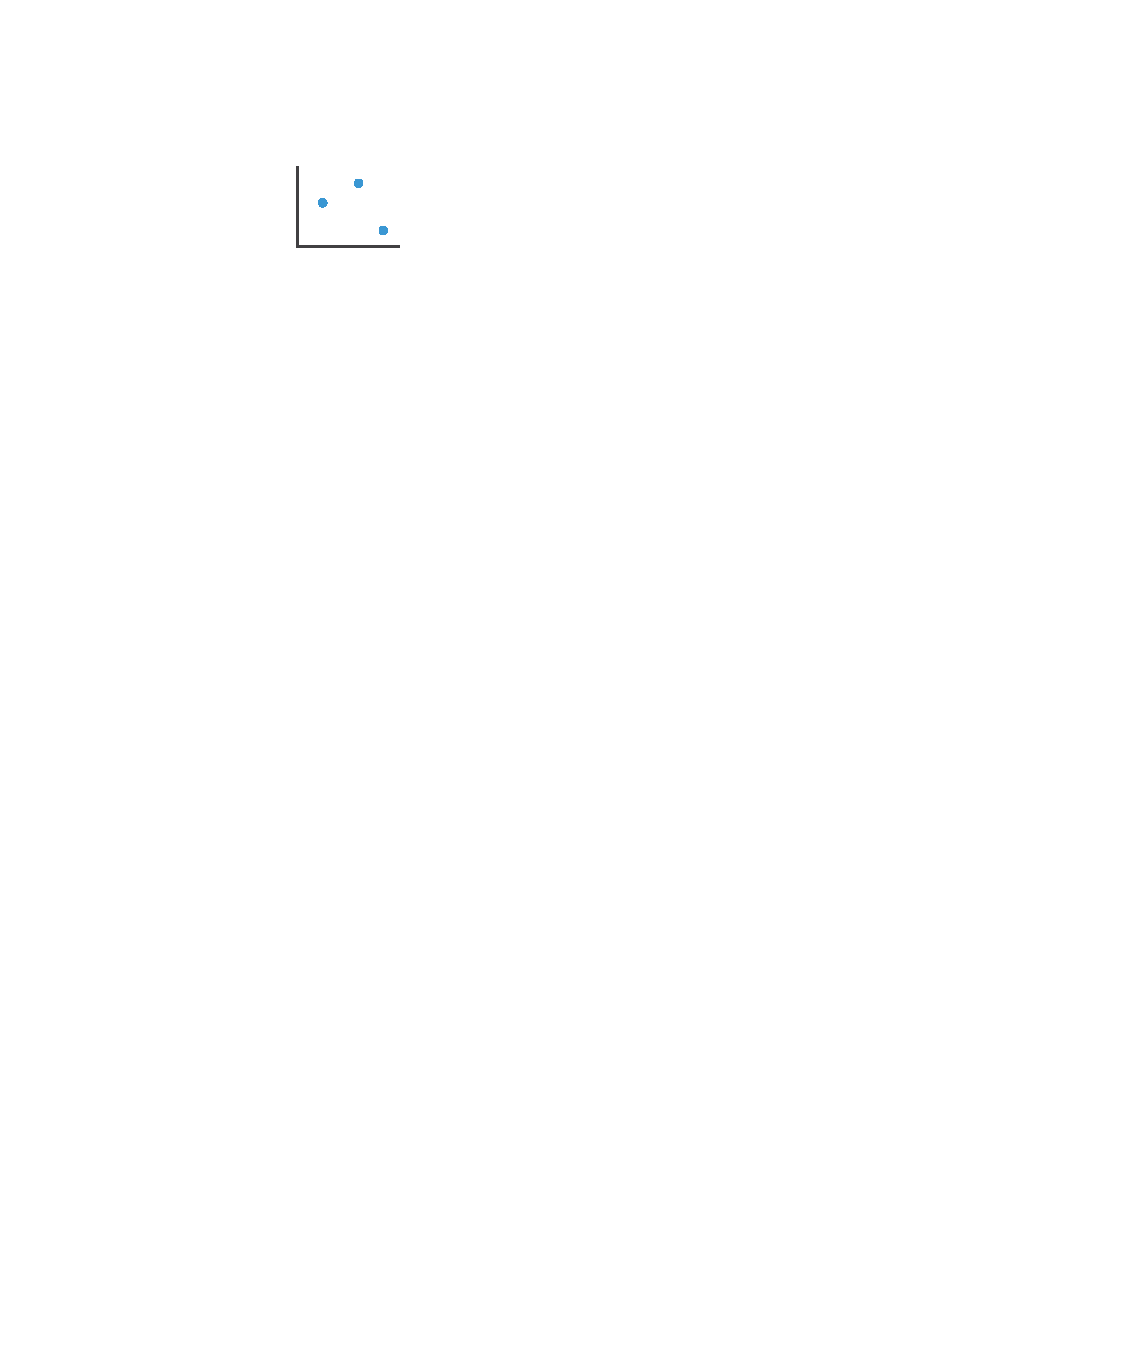
\includegraphics[width=.23\columnwidth]{channel-example-2}} 
\hfill
\subcaptionbox{A categorical attribute is added using the color channel.\label{fig:lr-channel-example-3}}{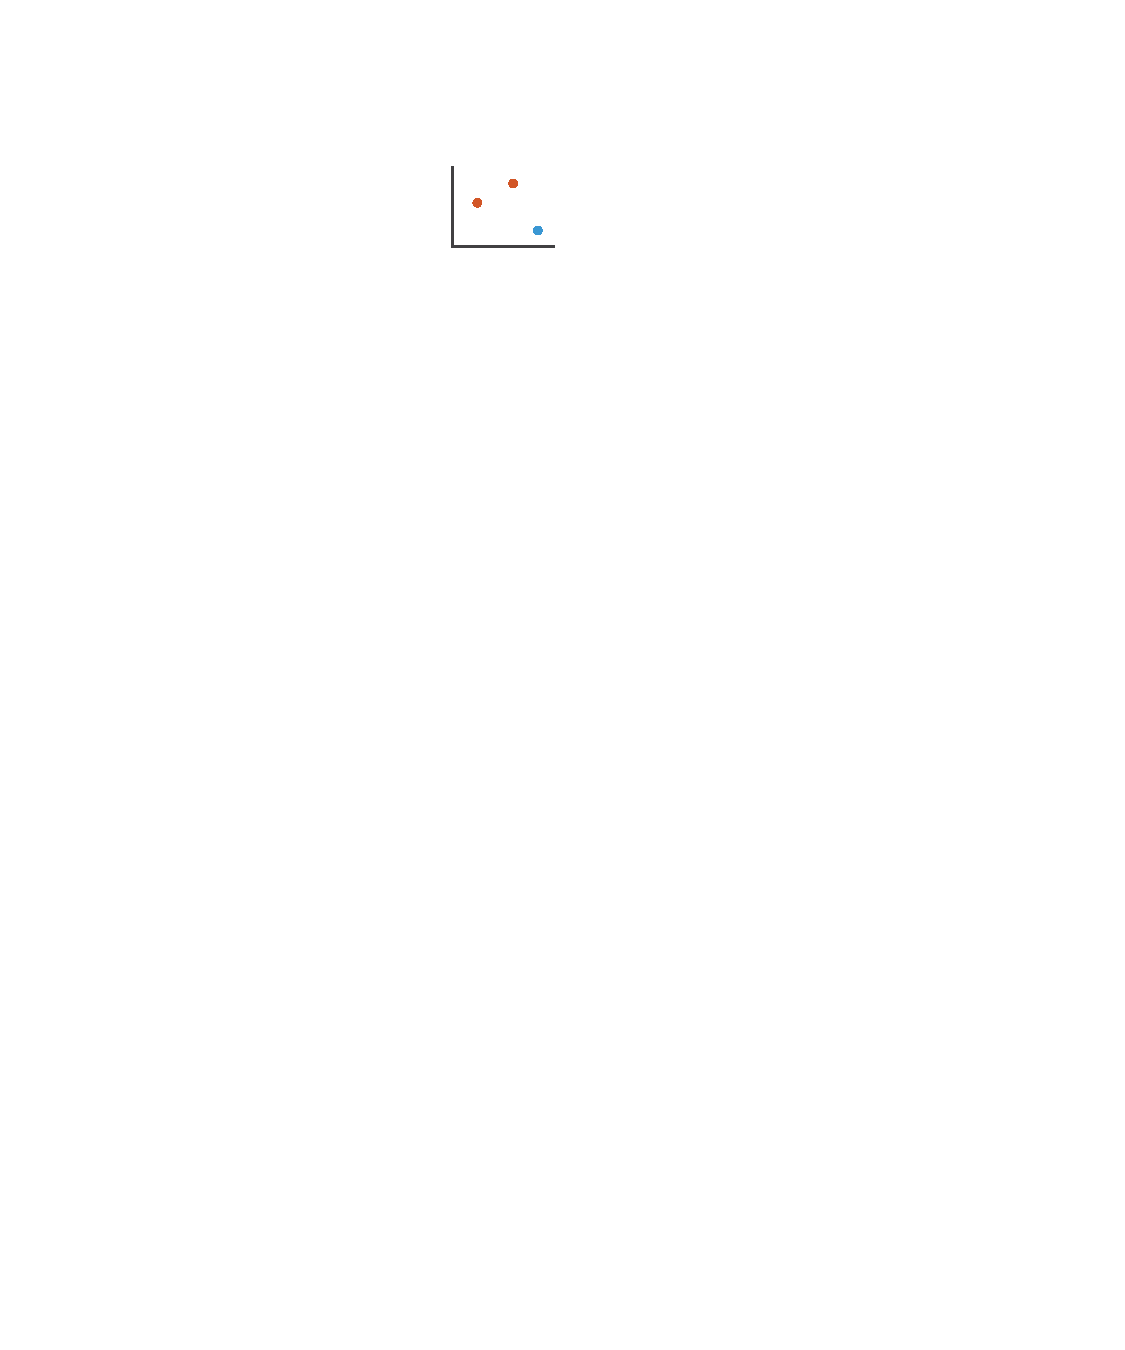
\includegraphics[width=.23\columnwidth]{channel-example-3}}
\hfill
\subcaptionbox{Another quantitative attribute is added using the size channel.\label{fig:lr-channel-example-4}}{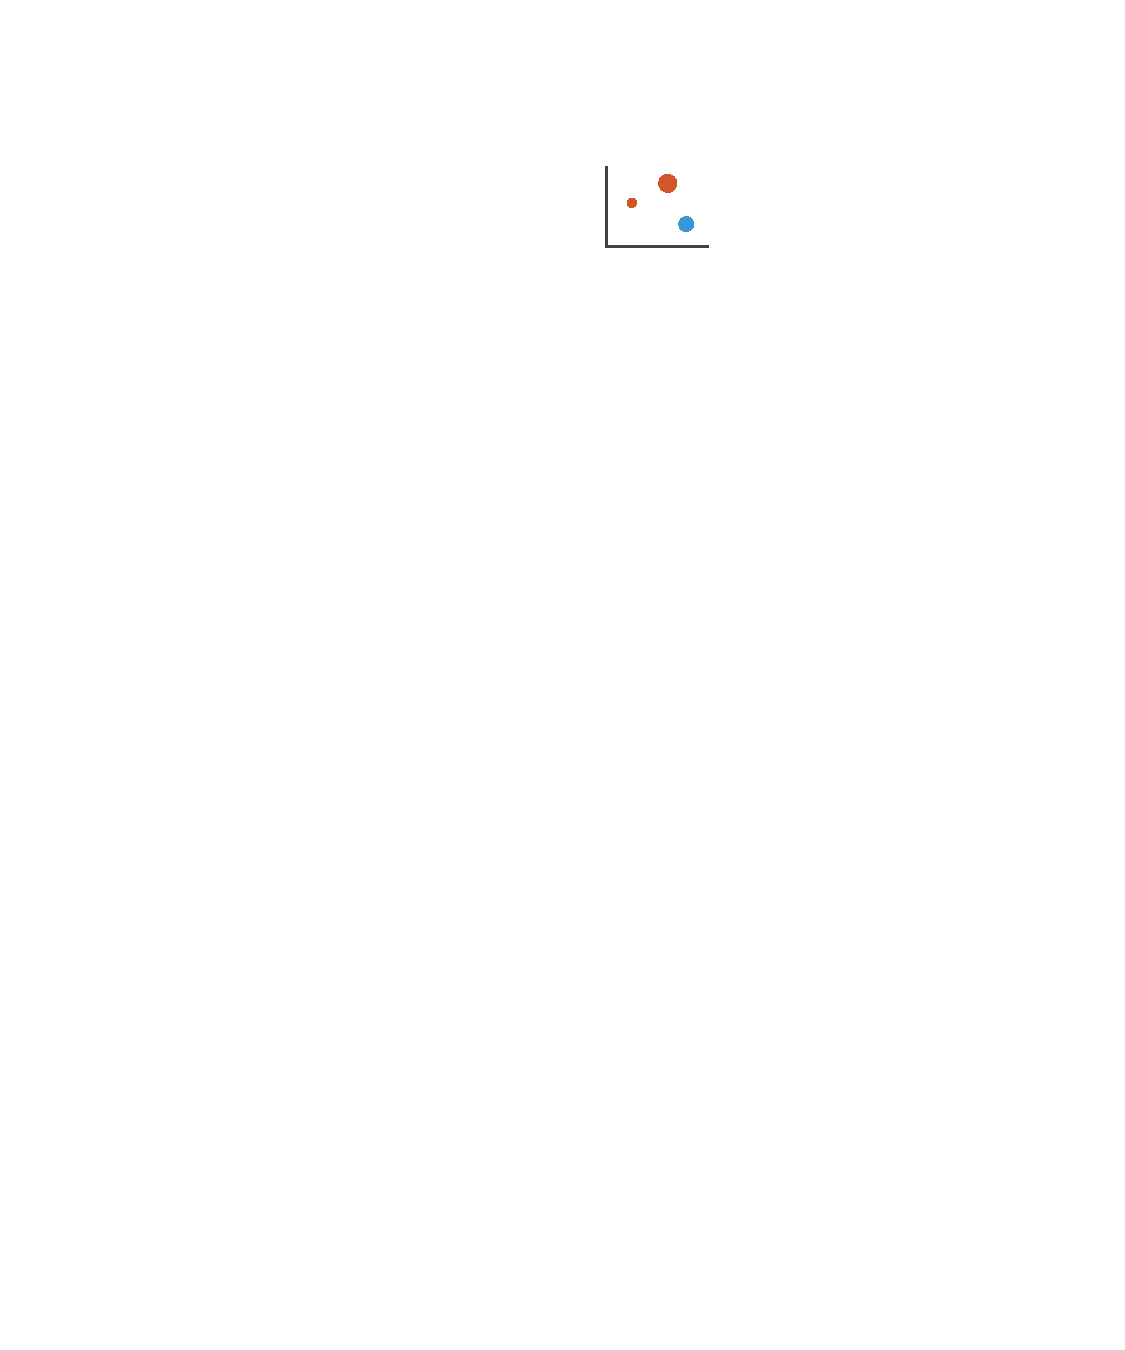
\includegraphics[width=.23\columnwidth]{channel-example-4}}
\caption{Using marks and channels.}
\label{fig:lr-channel-example}
\end{figure}

All channels are not equal; they are processed and perceived differently by our human visual systems. Also, not all channels are appropriate for encoding both ordered and categorical attributes. Ordered attributes should be shown using magnitude channels, with \emph{aligned spatial position} as the most effective channel and \emph{3D volume} as the least effective one. Categorical attributes should be shown using identity channels, with \emph{spatial region} as the most effective channel and \emph{shape} as the least effective one. \autoref{fig:lr-channel-ranking} shows the detailed ranking of effectiveness of many visual channels, separated by the type of attribute. This ranking is documented by Munzner~\cite{Munzner2014}, based on many empirical studies such as the work by Cleveland and McGill~\cite{Cleveland1985}, and by Heer and Bostock~\cite{Heer2010a}.

\begin{figure}[!htb]
	\centering
	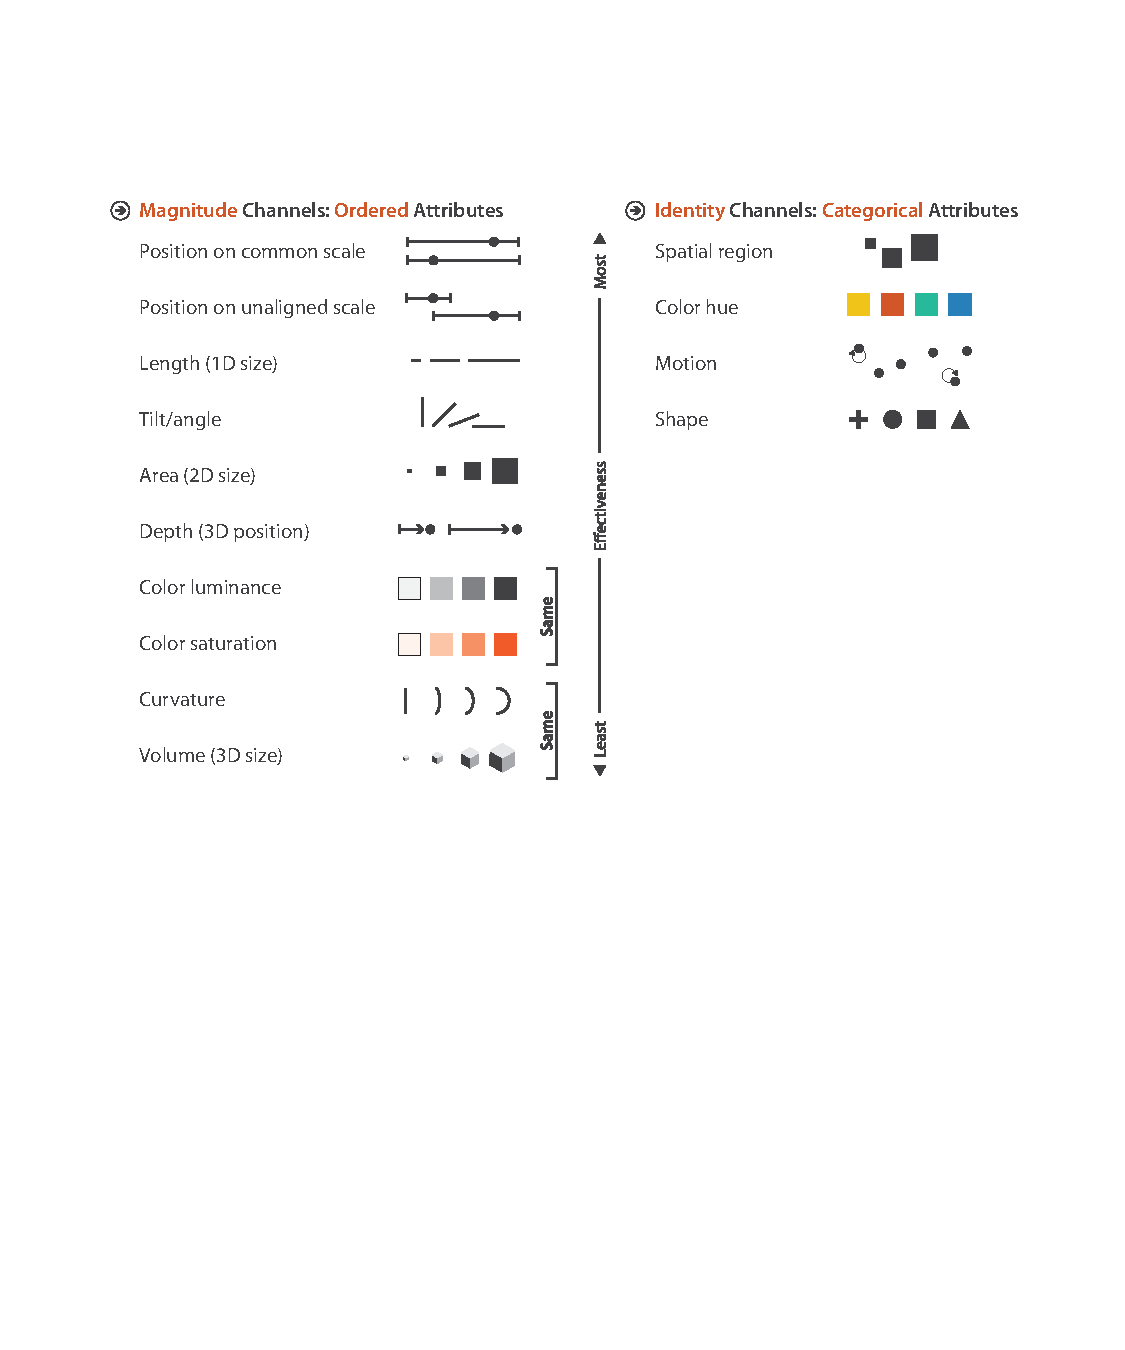
\includegraphics[width=\linewidth]{channel-ranking}
	\caption{Channels ranked by effectiveness according to data and channel type. \is{Munzner2014}}
	\label{fig:lr-channel-ranking}
\end{figure}

Color is a special channel that can be used for both data attributes. As shown in \autoref{fig:lr-channel-ranking}, color luminance and saturation are used in magnitude channels, and color hue is used in identity channels. A colormap specifies a mapping between colors and data values, and designing an effective colormap is challenging. ColorBrewer~\cite{Harrower2003} is an excellent source for colormap reference, providing color schemes for both categorical and ordered attributes. Human can only distinguish around 12 colors simultaneously~\cite{Munzner2014}. \autoref{fig:lr-colorbrewer-1} shows such a categorical colormap with 12 distinguished color hues. Ordered colormaps can be either sequential (\autoref{fig:lr-colorbrewer-2}) or diverging (\autoref{fig:lr-colorbrewer-3}). Diverging colormaps use two different color hues to emphasize values below and above the middle point.

\begin{figure}[!htb]
\centering
\subcaptionbox{Categorical colormap with distinguishable color hues.\label{fig:lr-colorbrewer-1}}[\columnwidth]{
\includegraphics[width=.6\columnwidth]{colorbrewer-1}} 
\\
\subcaptionbox{Sequential colormap: a single color hue with different saturation level.\label{fig:lr-colorbrewer-2}}[\columnwidth]{\hspace{-.15\columnwidth}
\includegraphics[width=.45\columnwidth]{colorbrewer-2}}
\\
\subcaptionbox{Diverging colormap: two color hues emphasizing positive and negative values.\label{fig:lr-colorbrewer-3}}[\columnwidth]{\hspace{-.05\columnwidth} 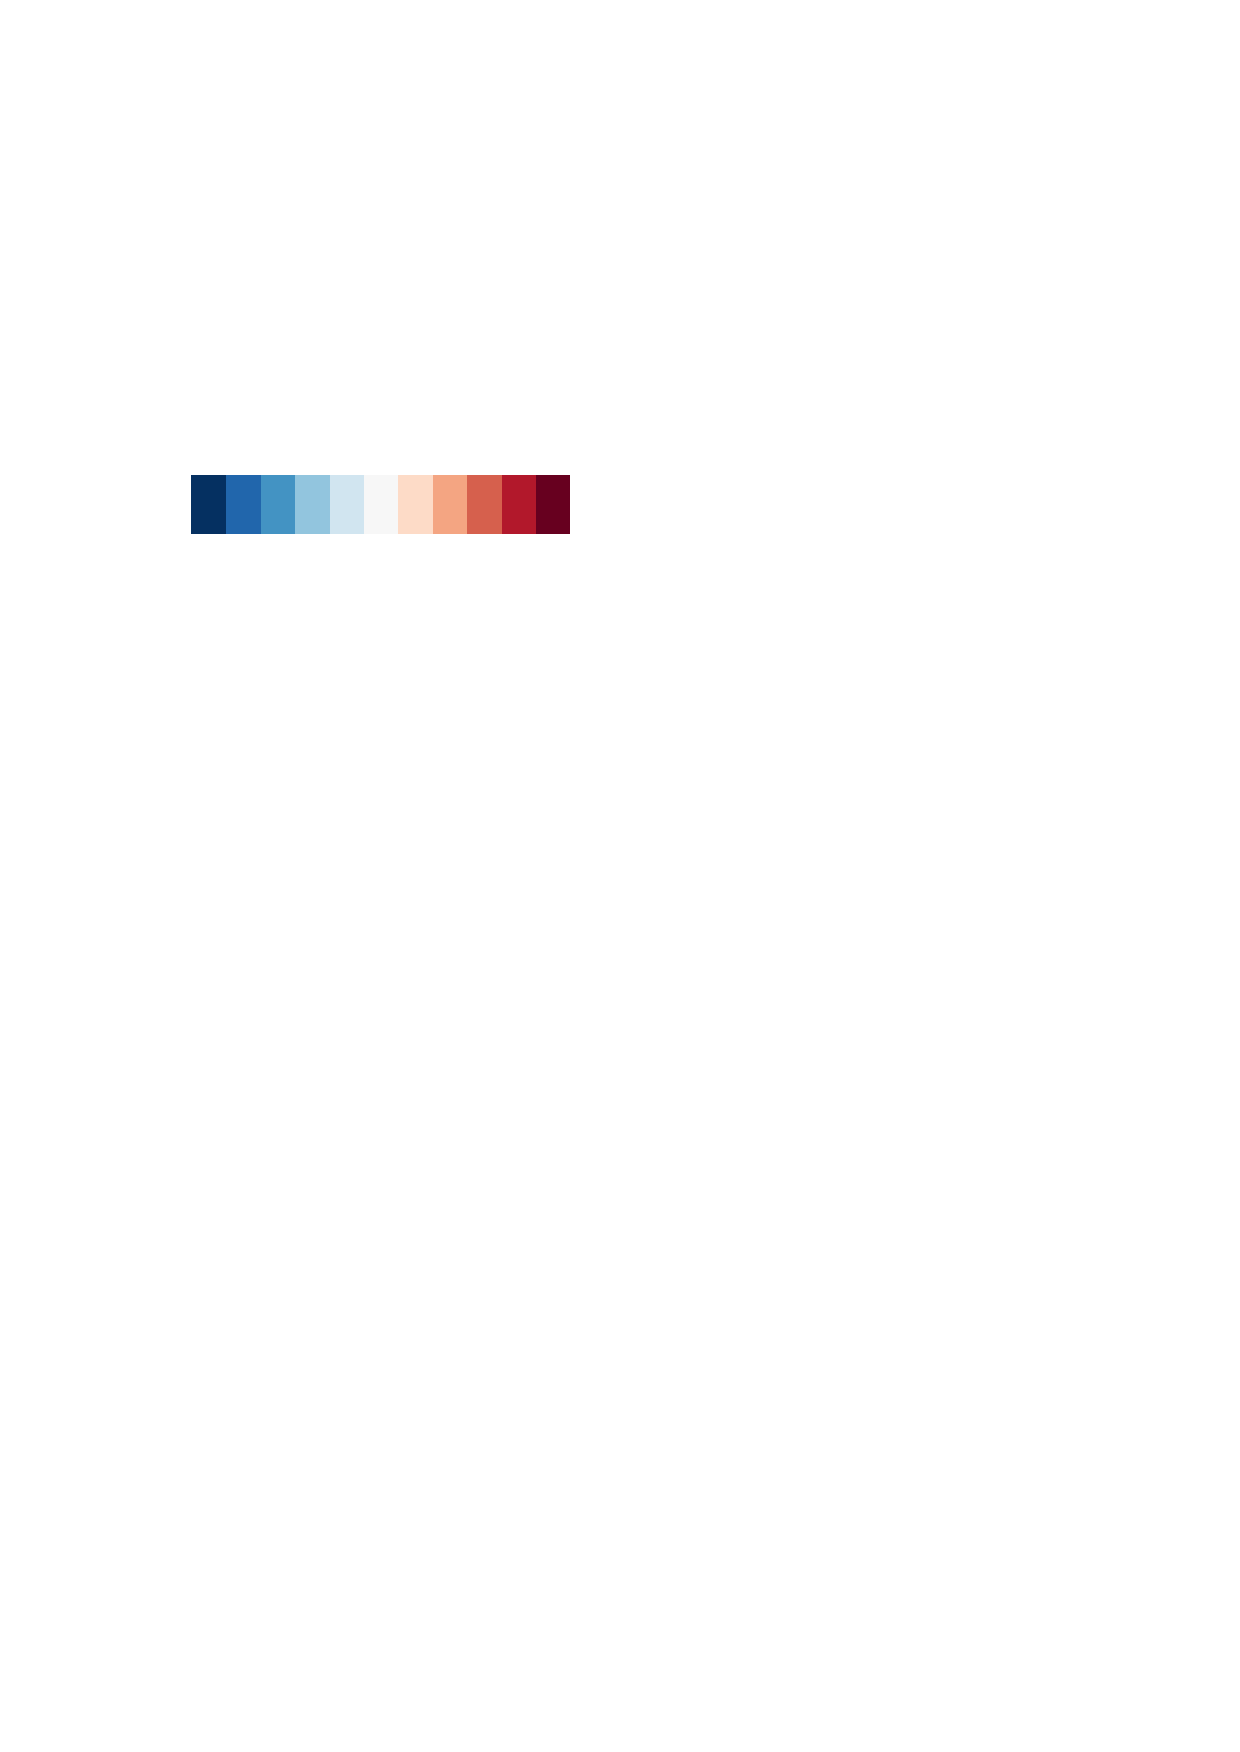
\includegraphics[width=.55\columnwidth]{colorbrewer-3}}
\caption{Colormaps from ColorBrewer. \is{Harrower2003}}
\end{figure}

\subparagraph{Gestalt Principles}
\label{sub:lr-gestalt}
Gestalt principles describe how we see patterns in visual displays~\cite{Koffka1935}. This section reviews three commonly used principles in representing groups of items.

\subparagraph{Similarity} 
Similar elements tend to be grouped together. \autoref{fig:lr-gestalt-similarity-1} shows a matrix of point marks with uniform spacing, but using two different shapes: dot and cross. The similarity of shapes helps us see the rows more clearly than the columns. Two separable channels can be applied together to reveal patterns by either rows or columns. In \autoref{fig:lr-gestalt-similarity-2}, green is used to depict rows, and texture is used to depict columns.

\begin{figure}[!htb]
\centering
\subcaptionbox{Similarity of shapes distinguishes rows.\label{fig:lr-gestalt-similarity-1}}[.47\columnwidth]{
\includegraphics[height=.35\columnwidth]{gestalt-similarity-1}} 
\hfill
\subcaptionbox{Color and texture delineate rows and columns, respectively.\label{fig:lr-gestalt-similarity-2}}[.47\columnwidth]{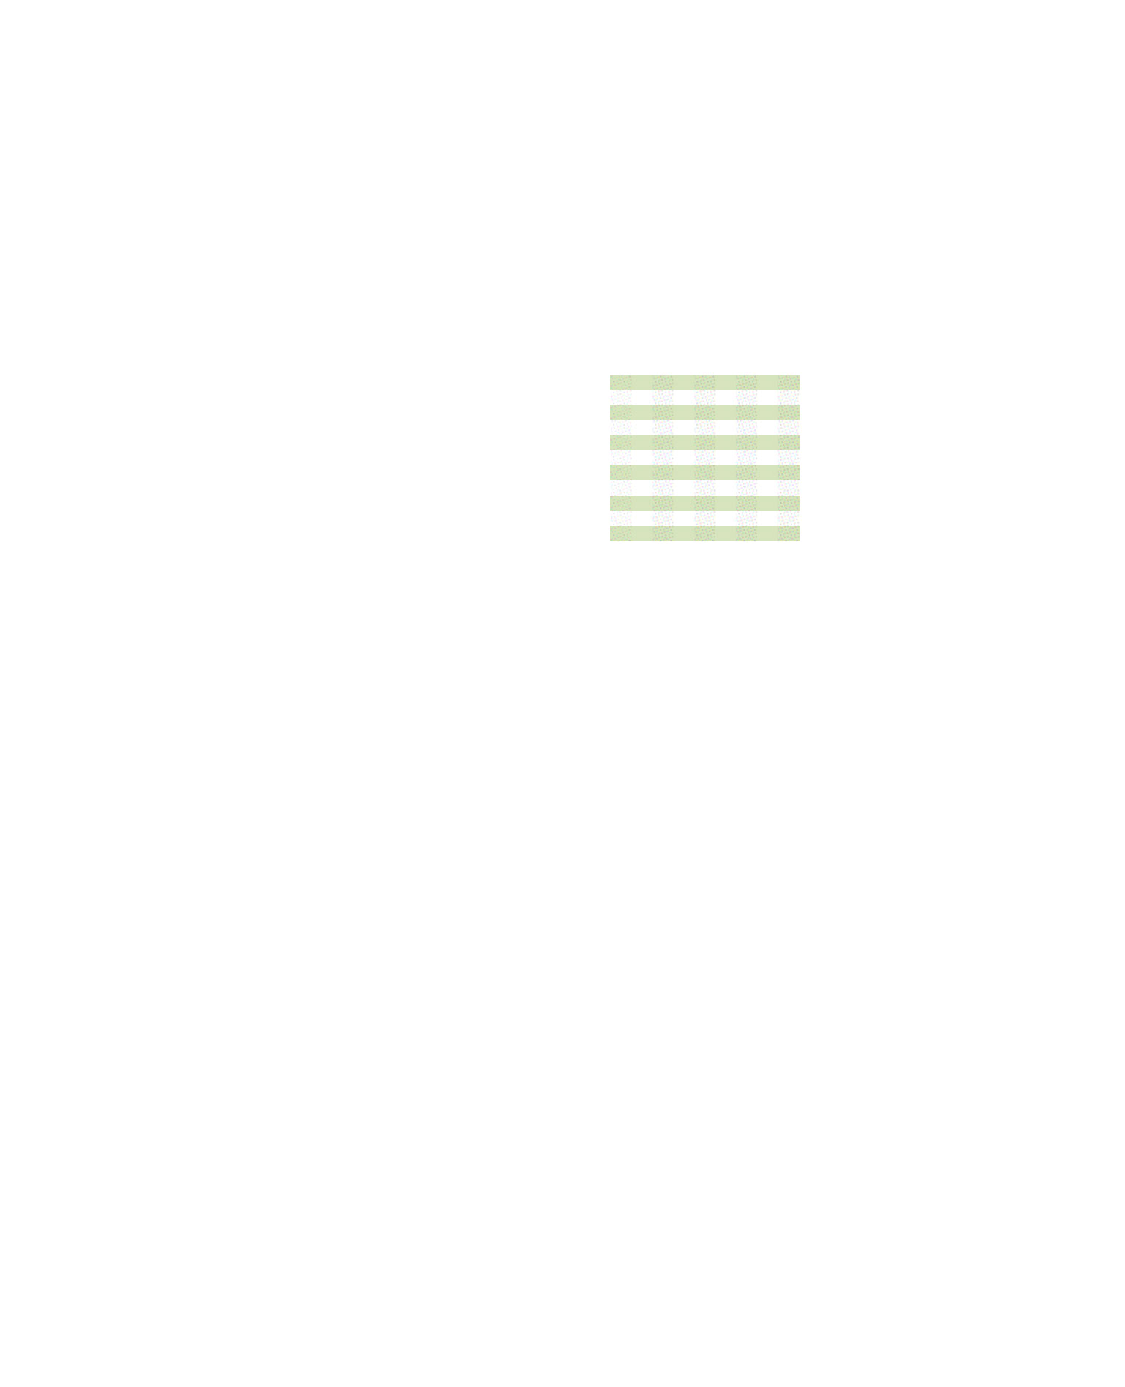
\includegraphics[height=.35\columnwidth]{gestalt-similarity-2}} \label{fig:lr-gestalt-similarity}
\caption{Similarity principle: similar elements are perceived as a group. \is{Ware2013}}
\end{figure}

\subparagraph{Proximity} 
Elements that are close together are perceptually grouped together. \autoref{fig:lr-gestalt-proximity-1} clearly shows two groups of dots. \autoref{fig:lr-gestalt-proximity-2} shows rows of dots. However, with a small change of spacing, these dots are perceived as columns in \autoref{fig:lr-gestalt-proximity-3}. The application of this principle is straightforward: organizing related information close together. It helps separate groups of unrelated objects and facilitates searching for information.

\begin{figure}[!htb]
\centering
\subcaptionbox{Two groups of dots.\label{fig:lr-gestalt-proximity-1}}{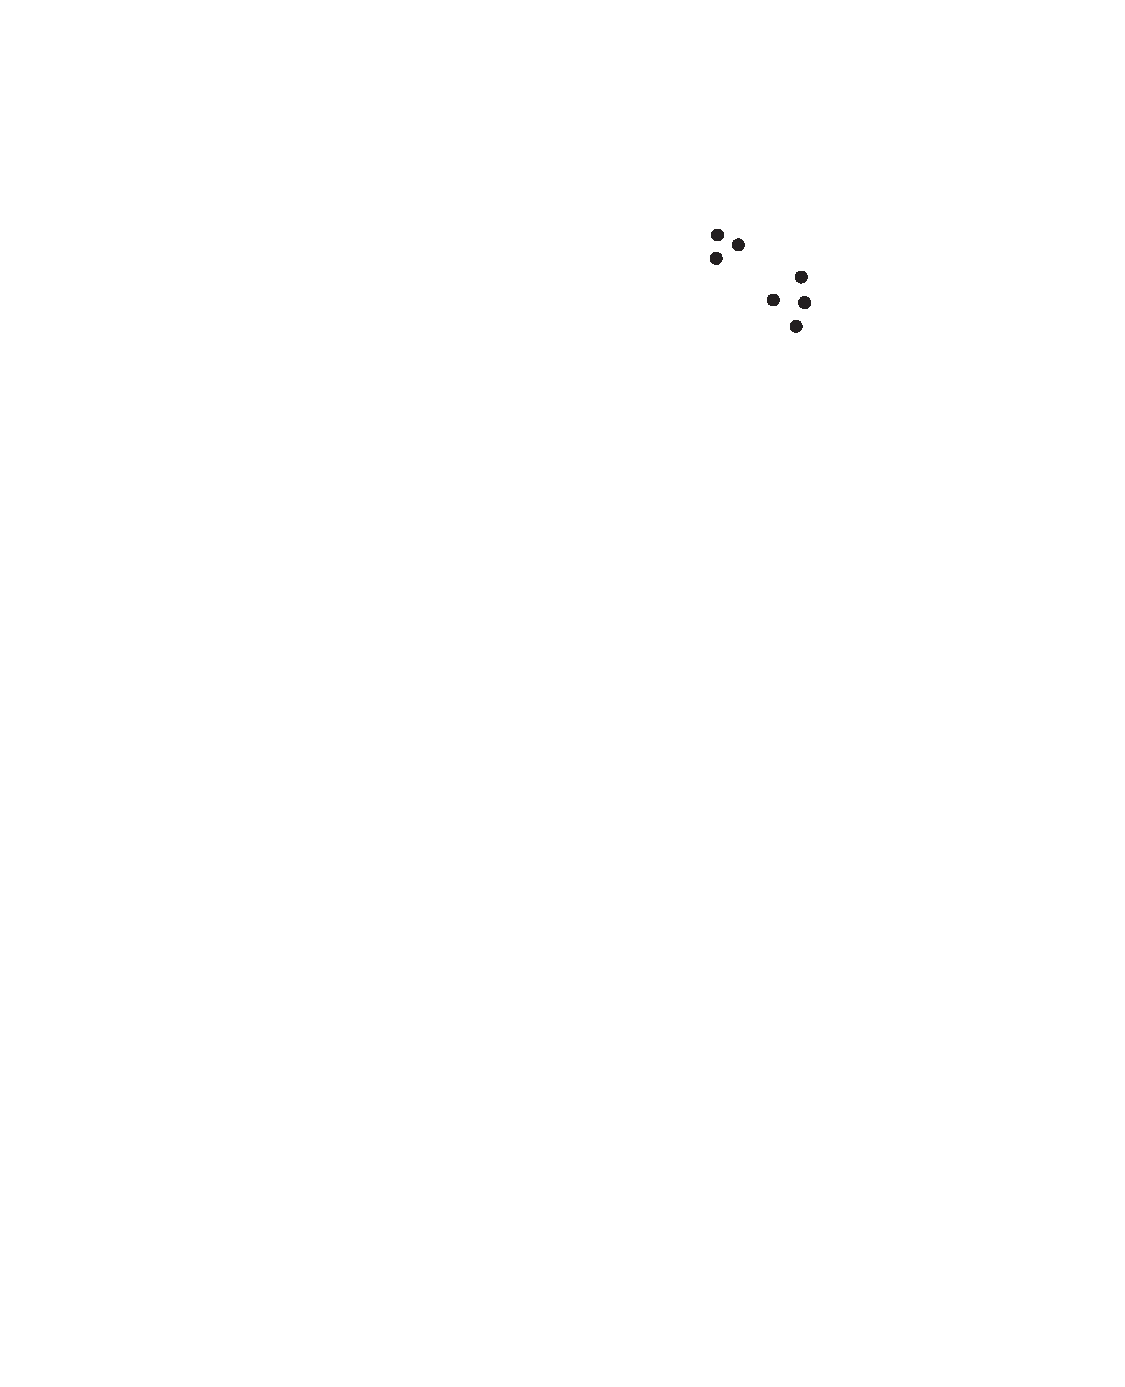
\includegraphics[width=.25\columnwidth]{gestalt-proximity-1}} 
\hfill
\subcaptionbox{Rows of dots.\label{fig:lr-gestalt-proximity-2}}{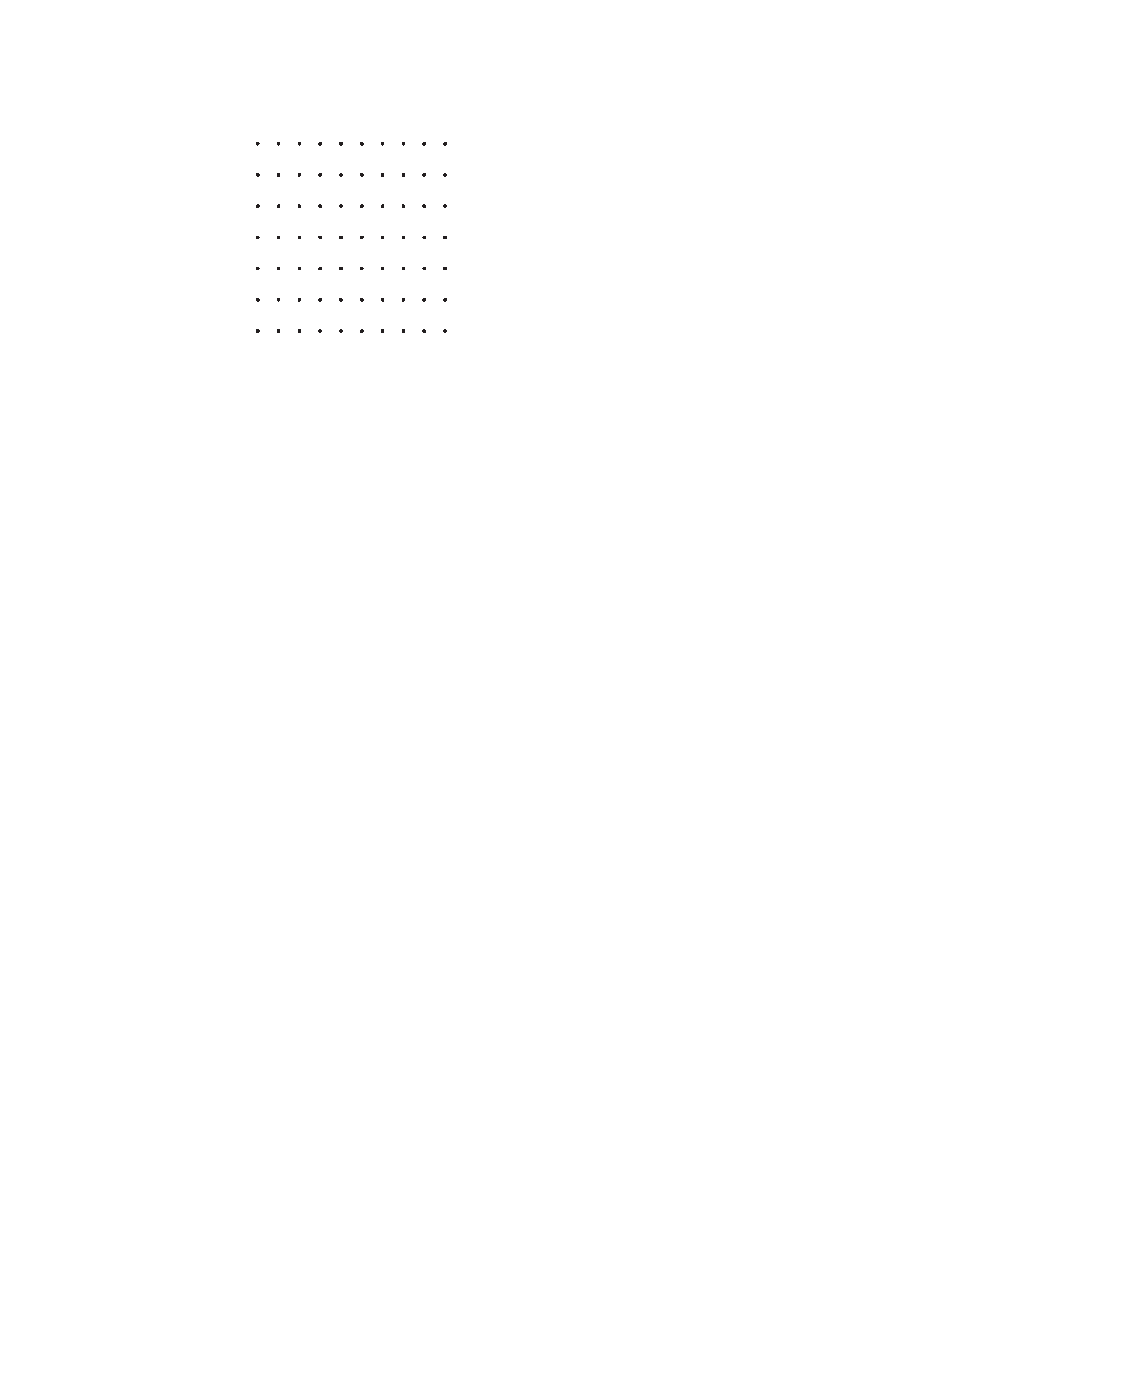
\includegraphics[width=.31\columnwidth]{gestalt-proximity-2}} 
\hfill
\subcaptionbox{Columns of dots.\label{fig:lr-gestalt-proximity-3}}{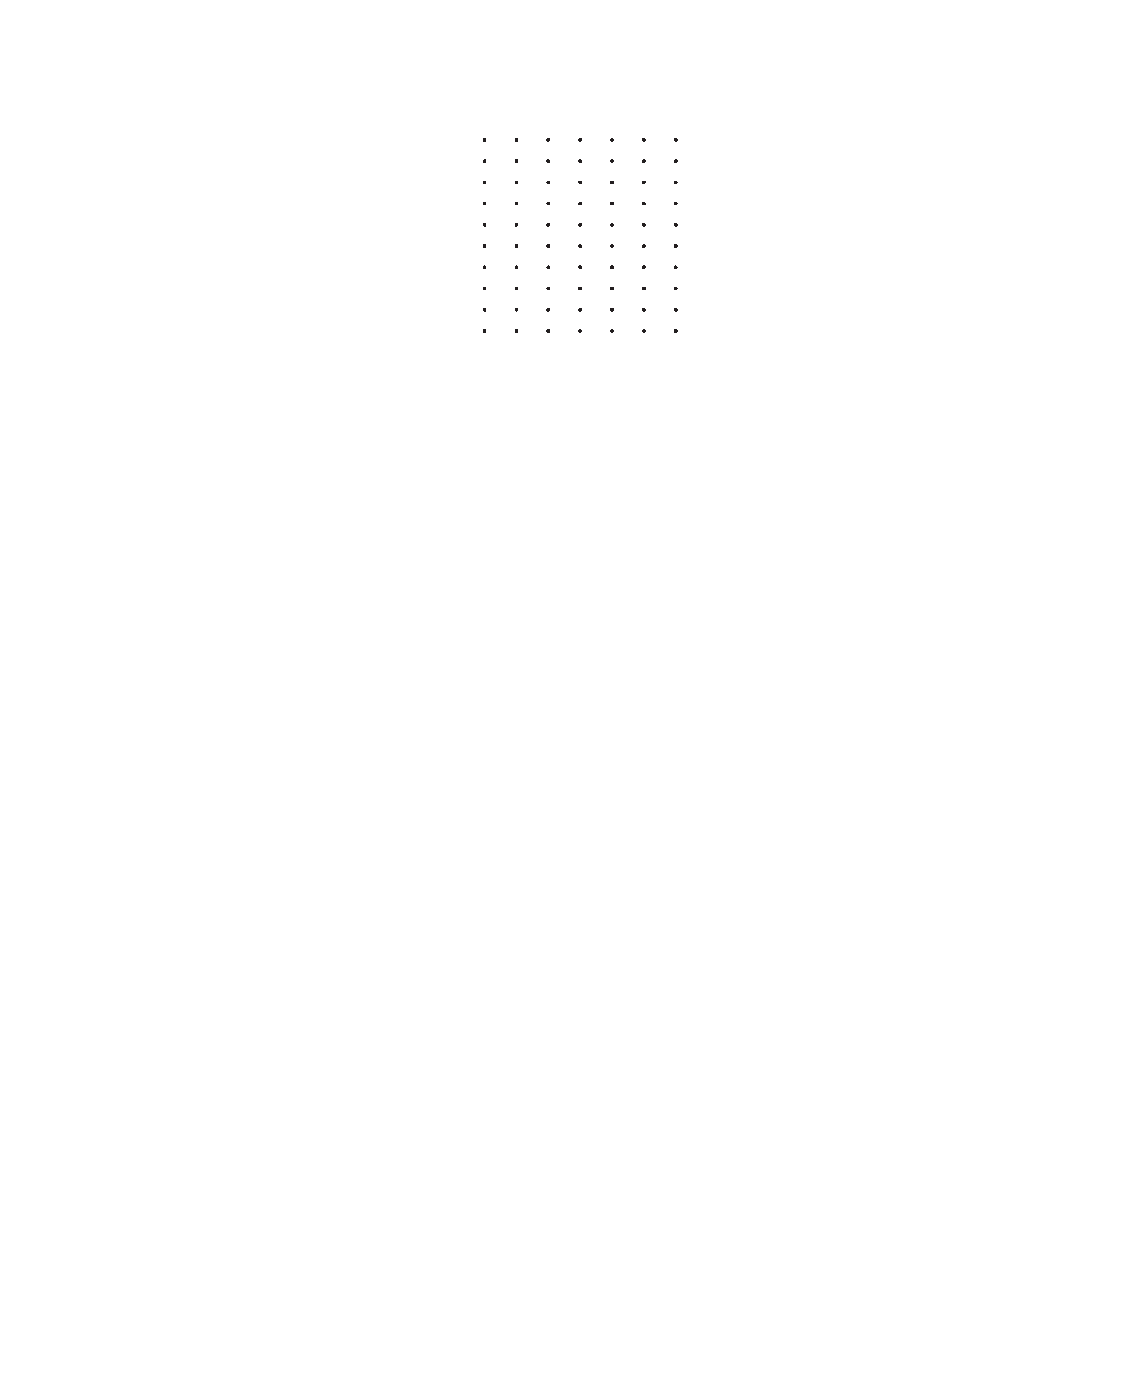
\includegraphics[width=.31\columnwidth]{gestalt-proximity-3}}
\label{fig:lr-gestalt-proximity}
\caption{Spatial proximity principle: spatially close elements are perceived as a group. \is{Ware2013}}
\end{figure}

\paragraph{Connectedness} 
Elements that are connected by visual properties are perceived as being more related than elements that are not connected. This principle can be achieved simply by drawing a border around a group of elements as in \autoref{fig:lr-gestalt-connectedness-1}. This is extensively applied in designing complex graphical user interface: groups of related features are separated by borders. Another approach to implement connectedness is by drawing lines between related elements as in \autoref{fig:lr-gestalt-connectedness-2}. This is the basics of \emph{node-link diagrams} -- one of the most common methods of representing relationships between elements.

\begin{figure}[!htb]
\centering
\subcaptionbox{Using border to denote a group.\label{fig:lr-gestalt-connectedness-1}}{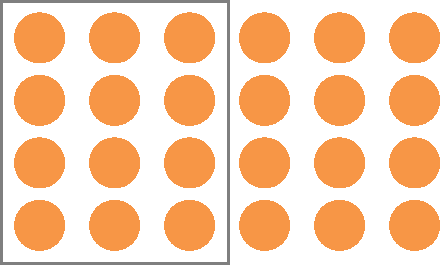
\includegraphics[width=.4\columnwidth]{gestalt-connectedness-1}} 
\hfill
\subcaptionbox{Using lines to denote a group.\label{fig:lr-gestalt-connectedness-2}}{
\includegraphics[width=.4\columnwidth]{gestalt-connectedness-2}} 
\caption{Connectedness principle: visually connected elements are perceived as a group. \is{Ware2013}}
\label{fig:lr-gestalt-connectedness}
\end{figure}

Among these three Gestalt principles of representing groups of elements, connectedness has the strongest effect, followed by proximity and then similarity. \autoref{fig:lr-gestalt} illustrates this comparison. In \autoref{fig:lr-gestalt-1}, even though spacing between dots in rows is shorter than spacing between dots in columns, the lines make the vertical links clearer than rows. In \autoref{fig:lr-gestalt-2}, the lines also make the horizontal links more notable than groups of colored circles. In \autoref{fig:lr-gestalt-3}, two spatial groups are more clearly perceived than colored groups.

\begin{figure}[!htb]
\centering
\subcaptionbox{Links are more clearly perceived than spatial groups.\label{fig:lr-gestalt-1}}[.3\columnwidth]{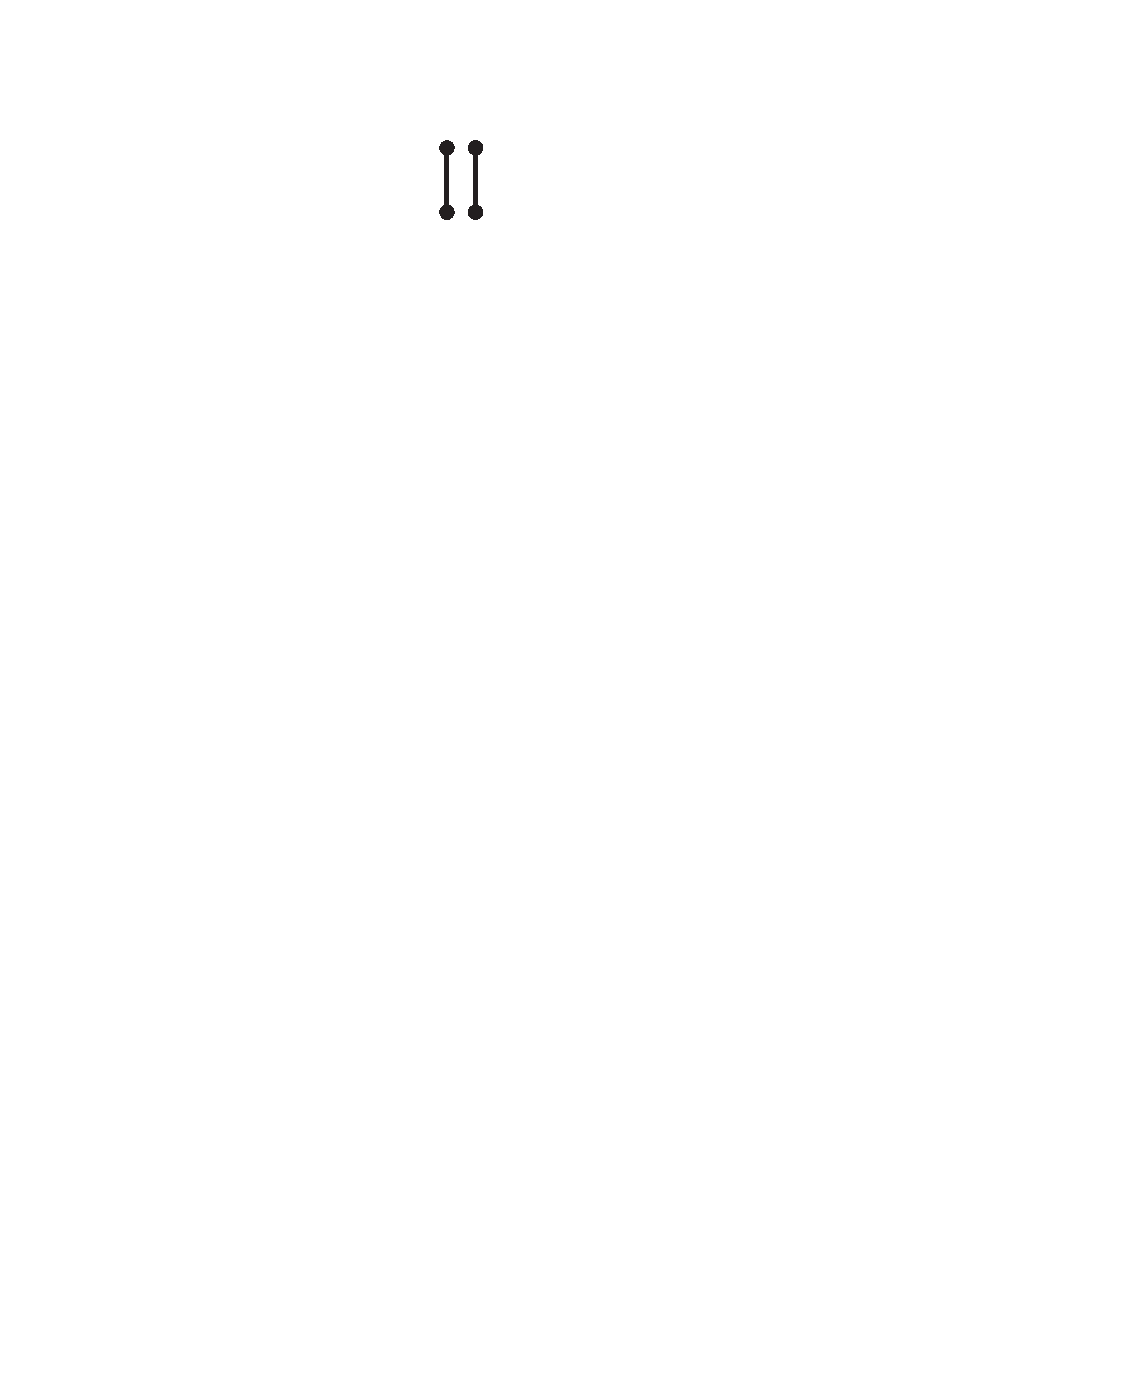
\includegraphics[height=.12\columnwidth]{gestalt-1}} 
\hfill
\subcaptionbox{Links are more clearly perceived than colored groups.\label{fig:lr-gestalt-2}}[.3\columnwidth]{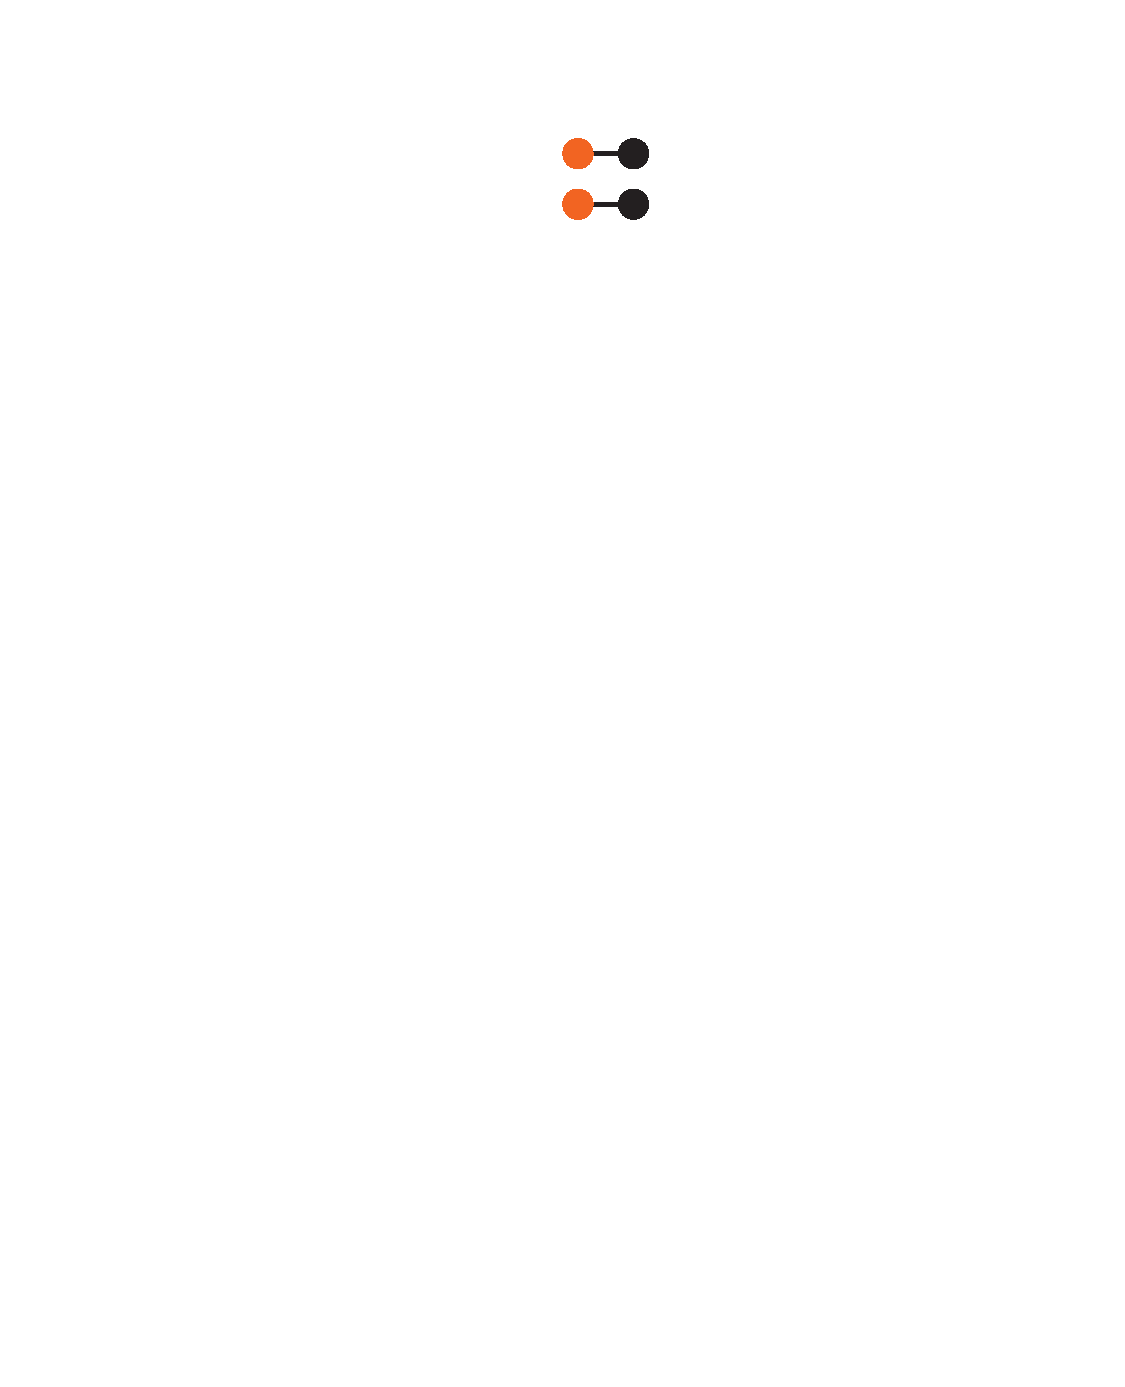
\includegraphics[height=.12\columnwidth]{gestalt-2}} 
\hfill
\subcaptionbox{Spatial groups are more clearly perceived than colored groups.\label{fig:lr-gestalt-3}}[.3\columnwidth]{
\includegraphics[height=.12\columnwidth]{gestalt-3}}
\caption{Comparison of Gestalt principles. Connectedness is stronger than proximity, and proximity is stronger than similarity. \is{Ware2013}}
\label{fig:lr-gestalt}
\end{figure}

\paragraph{Tufte's Principles}
Tufte proposes a number of principles for a well-designed graphic, documented in his series of books, most notably including \emph{The Visual Display of Quantitative Information}~\cite{Tufte1983} and \emph{Envisioning Information}~\cite{Tufte1990}. This section reviews a few principles that have been commonly applied in graphic design and visualization.

\subparagraph{Graphical Integrity}
This principle emphasizes that the graphical representation should tell the truth about the data. Representation of numbers, as physically measured on the surface of the	graphic	itself,	must be directly proportional to the numerical quantities represented~\cite{Tufte1983}. \autoref{fig:lr-tufte-integrity-1} shows a falsely big drop in stock market value between 2001 and 2002. It because the chart uses a relative scale with the value range from 450 to 500, causing its height disproportional to the market value. \autoref{fig:lr-tufte-integrity-2} corrects this error by using an absolute scale with the value range starting from 0.

\begin{figure}[!htb]
\centering
\subcaptionbox{Using a relative value range causes a falsely big drop of stock market value between 2001 and 2002.\label{fig:lr-tufte-integrity-1}}{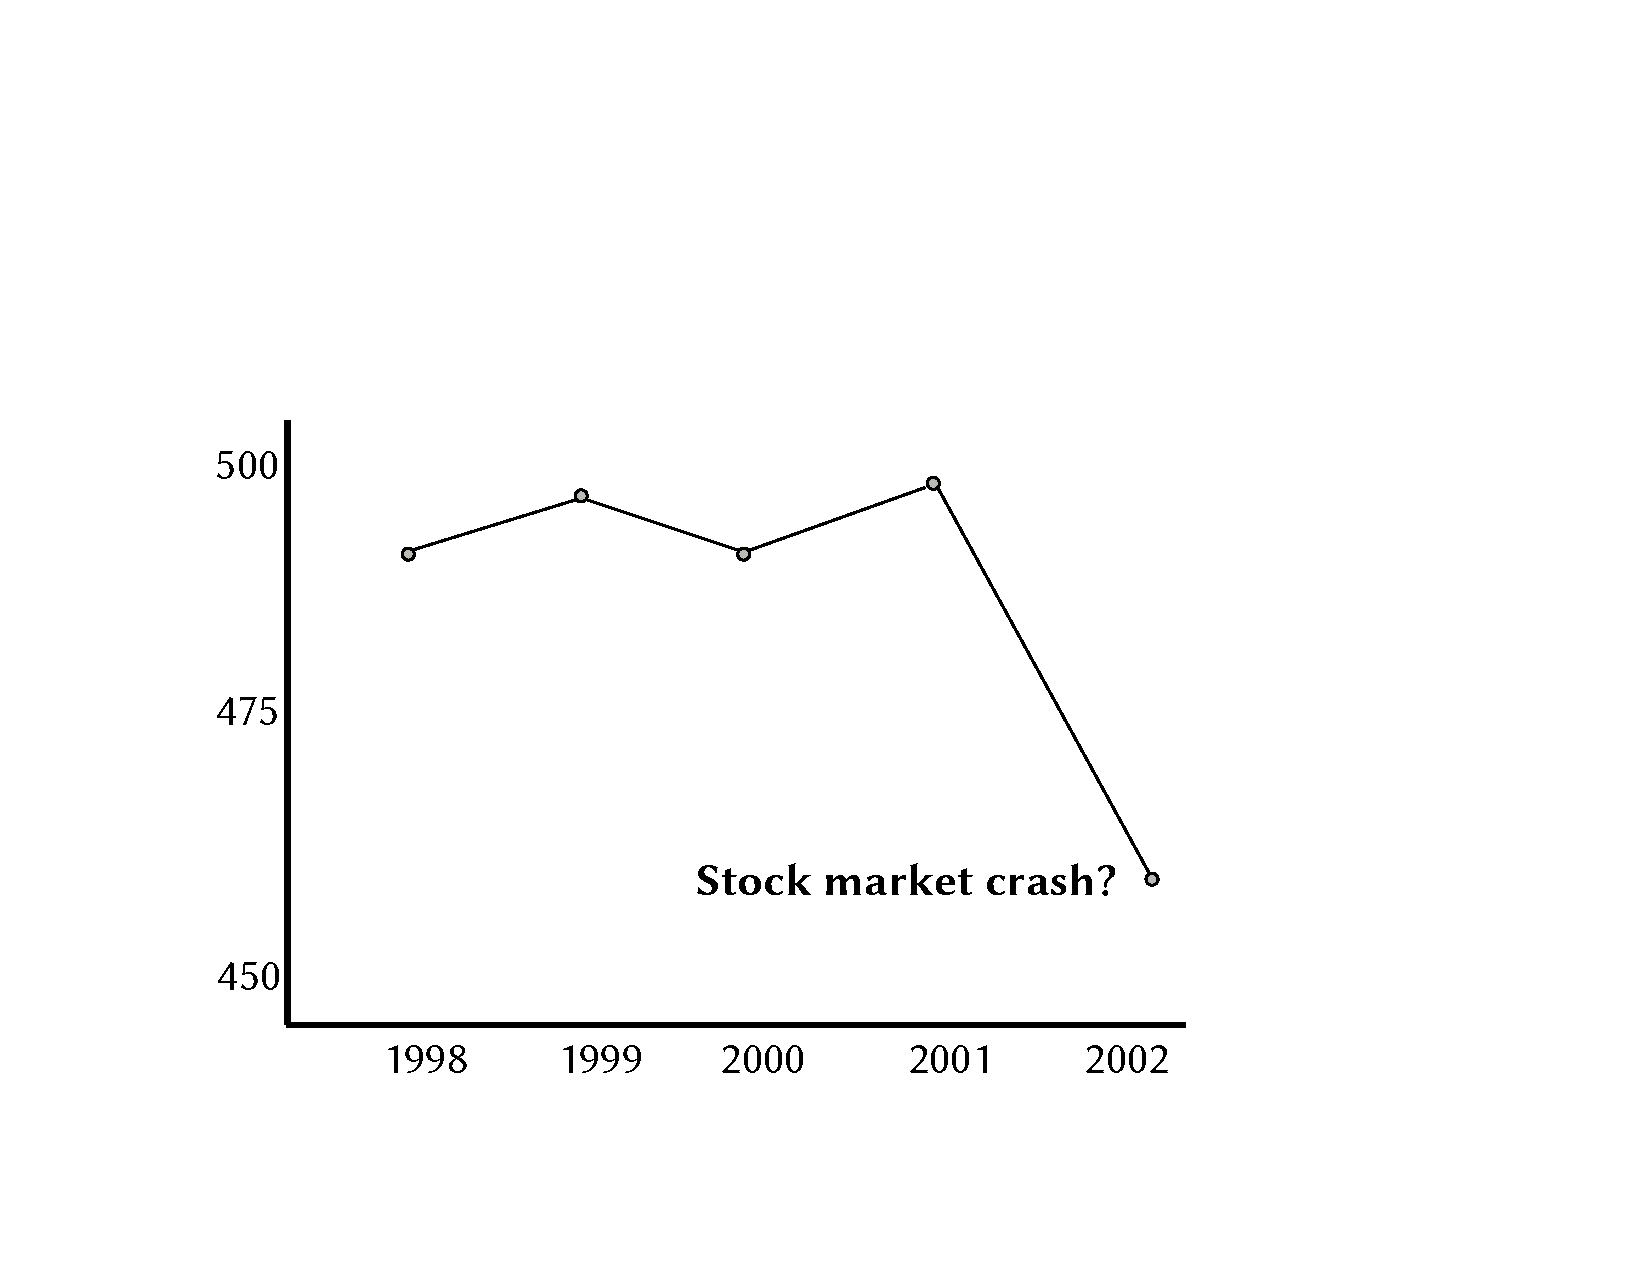
\includegraphics[width=.47\columnwidth]{tufte-integrity-1}} 
\hfill
\subcaptionbox{Using an absolute value range to depict the data accurately.\label{fig:lr-tufte-integrity-2}}{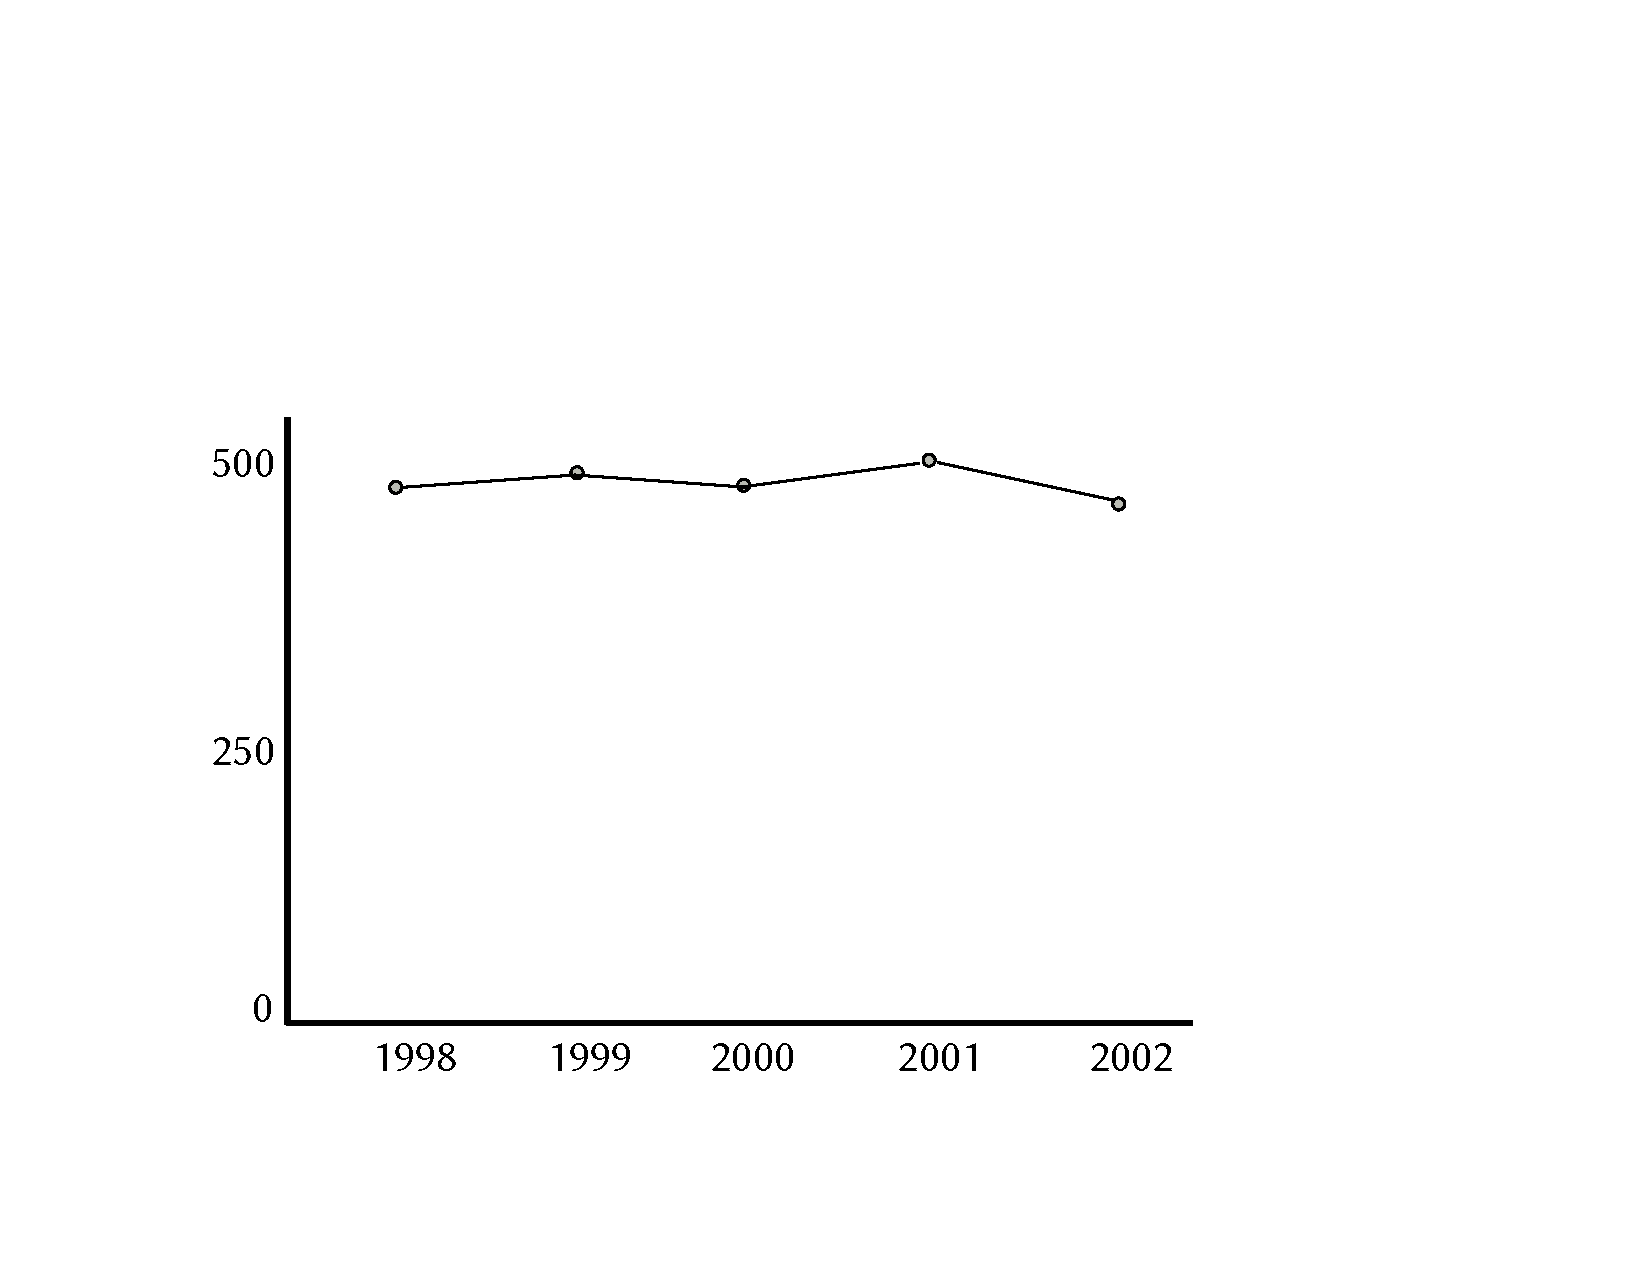
\includegraphics[width=.47\columnwidth]{tufte-integrity-2}} 
\caption{Graphical integrity principle. The chart should tell the truth about the data.}
\label{fig:lr-tufte-integrity}
\end{figure}

\subparagraph{Data-Ink Ratio Maximization}
Data-ink includes the pixels in the graphic that are used for representing the data. Data-ink ratio is defined as the ratio between the data-ink and the total non-background pixels used in the graphic. This principle aims to maximize this ratio by erasing non-data-ink and erasing redundant data-ink.

\begin{figure}[!htb]
\centering
\subcaptionbox{A bar chart with poor data-ink ratio.\label{fig:lr-tufte-ink-1}}{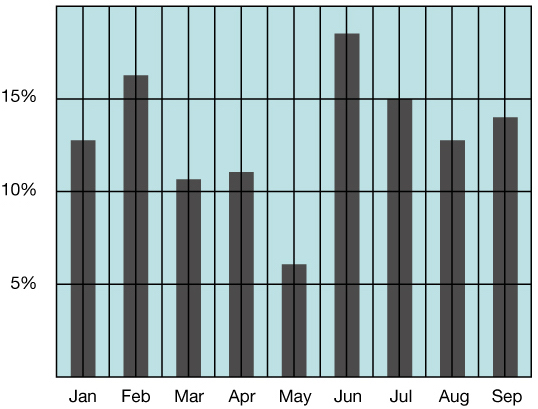
\includegraphics[width=.47\columnwidth]{tufte-ink-1}} 
\hfill
\subcaptionbox{A bar chart with high data-ink ratio by removing background, border and grid lines.\label{fig:lr-tufte-ink-2}}{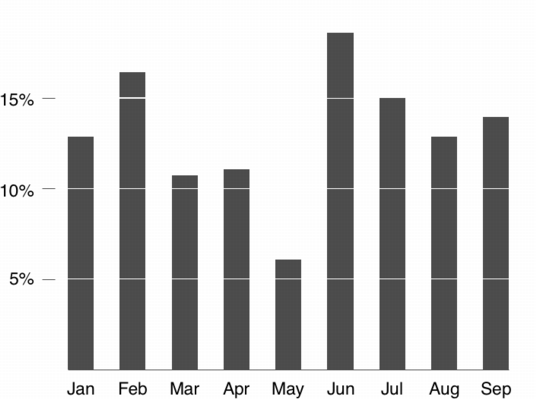
\includegraphics[width=.47\columnwidth]{tufte-ink-2}} 
\caption{Data-ink ratio maximization principle: removing the graphic that does not contribute to the understanding of the data.}
\label{fig:lr-tufte-ink}
\end{figure}
% Source: http://www.infovis-wiki.net/index.php/Data-Ink_Ratio

\subparagraph{Micro/Macro Readings}
This principle suggests that a graphic can contain both enormous details and an overall pattern. This allows the viewer to glance from a distance to observe the big picture, and later drill-down closely to examine its individual pieces. Classic stem-and-leaf plot is a great example to illustrate this principle (\autoref{fig:lr-tufte-micro}). The plot shows all individual data items at meaningful level of detail, and provides an understanding of the data distribution. The micro/macro principle is extensively applied in interactive visualization, where zooming are panning are made possible, such as Google Maps. Data items at different scales can be represented with different levels of detail to provide appropriate information based on the allowed display area.

\begin{figure}[!htb]
	\centering
	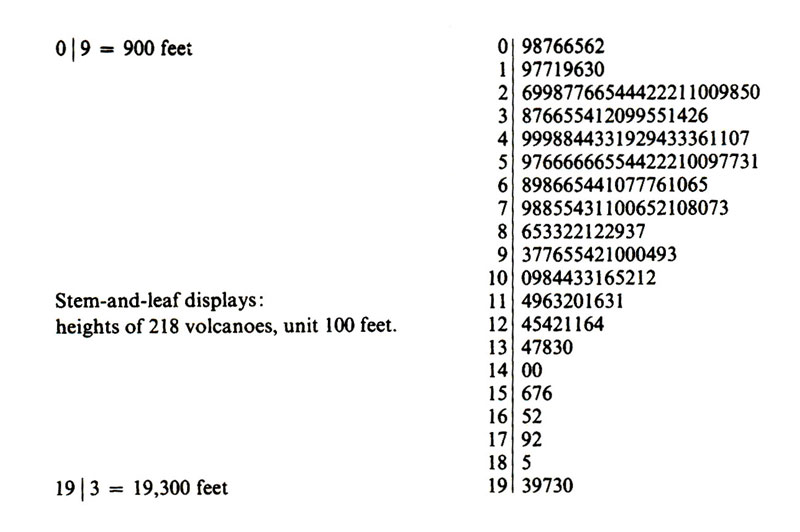
\includegraphics[width=.9\linewidth]{tufte-micro}
	\caption{Micro/macro principle. A stem-and-leaf plot shows both the data distribution and individual items. \is{Tufte1983}}
	\label{fig:lr-tufte-micro}
\end{figure}


%In a broader context, GUI design principles:  Schneiderman~\cite{Shneiderman2016} (eight golden rules), Norman (six design principles) ~\cite{Norman2002} and	Nielsen (ten usability heuristics)~\cite{Nielsen1994} -- create a table with rows showing similar principles
%http://www.csun.edu/science/courses/671/bibliography/preece.html
%https://faculty.washington.edu/jtenenbg/courses/360/f04/sessions/schneidermanGoldenRules.html
%https://www.interaction-design.org/literature/article/shneiderman-s-eight-golden-rules-will-help-you-design-better-interfaces

\subsubsection{Interaction Techniques}
Interaction typically refers to the set of controls provided to the user to manipulate an interface~\cite{Pike2009a}. A static visualization may only show one aspect of a dataset. When the dataset is large enough, showing all the data at once may also make the visualization become cluttered. Interaction plays an important role in solving these problems. It can help explore large datasets at multiple levels of detail, identify patterns through examination of different visual representations and understand the connections between them.

Examples of interaction include standard techniques used in graphical user interface such as mouse clicking and scrolling, and more visualization specific techniques such as \emph{linking and brushing}~\cite{Kosara2003}, and \emph{focus+context}~\cite{Cockburn2008}. Multiple views in a visualization are often linked together to exploit their strengths. The user can select points of interest using the brushing technique, typically done directly on the visual data representation such as dragging a rectangular area. The points are brushed in one view will be highlighted in other views, allowing the user to explore them with different perspectives and representations (\autoref{fig:lr-linking}). Focus+Context is a technique that brings both the overview (context) and the detailed information (focus) together in one view. A fisheye view~\cite{Furnas1986,Furnas2006} is one example of this technique: the focal region is magnified and displayed within its surrounding context (\autoref{fig:lr-fisheye}).

\begin{figure}[!htb]
\centering
\subcaptionbox{Linking and brushing. Data points brushed in one view are linked and highlighted in other views.\label{fig:lr-linking}}{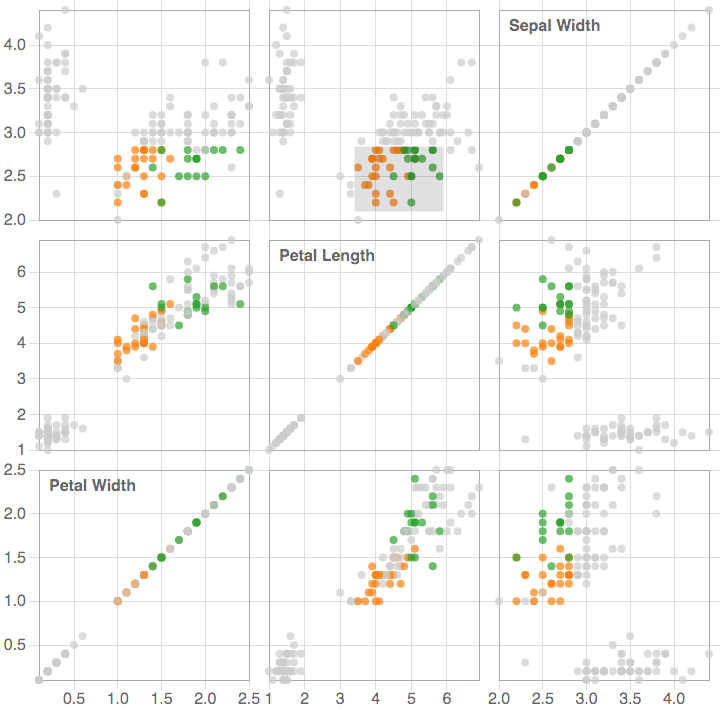
\includegraphics[height=.43\columnwidth]{linking}} 
\hfill
\subcaptionbox{Fisheye view for focus+context. Both the overview and the detailed information are displayed in one view.\label{fig:lr-fisheye}}{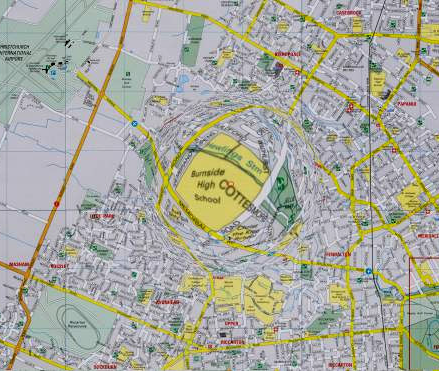
\includegraphics[height=.43\columnwidth]{fisheye}} 
\caption{Examples of interaction techniques.}
\label{fig:lr-interaction}
\end{figure}

Many other interaction techniques can be found in the taxonomies by Dix and Ellis~\cite{Dix1998}, by Keim~\cite{Keim2002}, and by Wilkinson~\cite{Wilkinson2005}. Very often, a user performs an interaction to achieve some goal, thus interaction techniques can also be classified based on their intents. Actually, different interaction techniques in different visualizations may serve the same purpose. For example, both drilling-down a treemap~\cite{Shneiderman1992} and semantic zooming~\cite{Perlin1993} aim to get more details. Taxonomies of high-level interaction can be found in the work by Yi~et~al.~\cite{Yi2007}, by Heer and Shneiderman~\cite{Heer2012}, and by Brehmer and Munzner~\cite{Brehmer2013}. These classifications could help visualization designers select suitable interaction techniques to serve for the capabilities they want to offer to the users.

%Several methods can improve existing different interaction techniques. 
Traditional graphical user interface widgets are often used to control different settings of a visualization, such as buttons and sliders. The disadvantage is that visual feedback does not appear where the interaction happens, but in some parts of the visualization. It also takes time for the user to search for the appropriate setting controllers. Direct manipulation~\cite{Shneiderman1982} is an approach to address these problems. It enables the user to directly interact with the visual representation and receive immediate feedback. One example is using mouse scrolling to adjust zoom level while exploring a map instead of clicking on a button in the toolbar. Another example is parallel coordinates plot with axes can be reordered by direct dragging and values can be filtered by direct brushing on the axes (\autoref{fig:lr-pcp}). Surrogate objects can be used when the data objects are small or distant~\cite{Kwon2011}. An example is the use of interactive legends as filtering means~\cite{Riche2010b}

\begin{figure}[!htb]
	\centering
	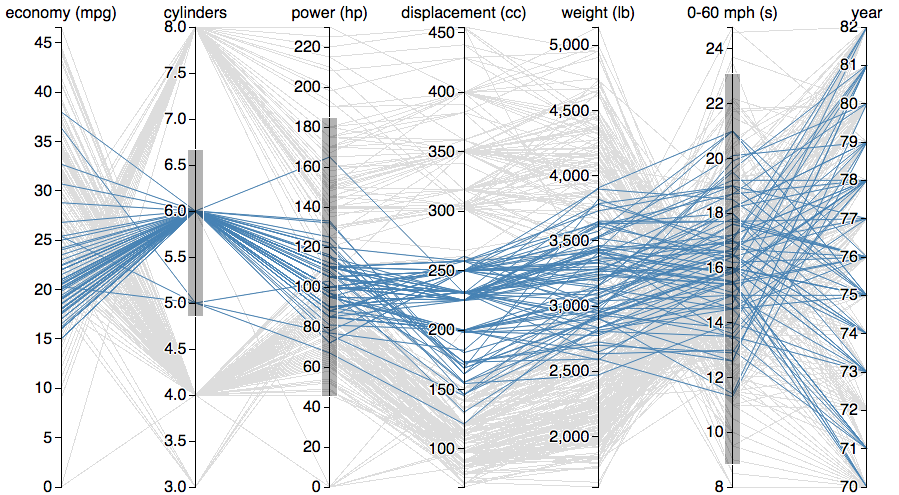
\includegraphics[width=\linewidth]{pcp}
	\caption{Direct manipulation in a parallel coordinates plot with reorder-able and brush-able axes.}
	\label{fig:lr-pcp}
\end{figure}

Another concept that can be applied to improve existing interaction techniques is \emph{fluid interaction}~\cite{Elmqvist2011}. Besides using direct manipulation as discussed previously, the interaction should produce smooth animated transitions between the state before and the state after an interaction, helping users maintain their mental maps; and provide immediate visual feedback, allowing users to know what is happening and/or what will happen next.

Typically, interaction techniques are combined to explore the data or present a known story. A classic visual information-seeking mantra by Shneiderman~\cite{Shneiderman1996} summarizes many design guidelines and interaction techniques for designing information visualizations: \emph{Overview first, zoom and filter, then details-on-demand}. With large datasets, it it challenging to create an overview and provides cues for further exploration. A more suitable approach in this case is \emph{Search, show context, expand on demand}~\cite{VanHam2009}.

\subsection{Automated Analysis Methods}
Data mining is the computational process of extracting patterns in large datasets~\cite{Tan2006}. Data mining tasks can be broadly divided into two major categories:

\begin{itemize}
		\item \emph{Descriptive tasks}. The objective is to derive patterns (correlations, trends, clusters, trajectories and anomalies) that summarizes the underlying relationships in data. Examples include cluster and association analyses. \emph{Clustering} aims to split data items to groups so that items within a group are more similar to each other than those in other groups. For example, clustering can be used to help marketers discover distinct groups of their customers before applying appropriate marketing strategies to those groups. \emph{Association} analysis discovers the connections among a set of data items. For example, it can be used to identify products that customers often purchase together such as bread and milk.
		
		\item \emph{Predictive tasks}. The objective is to predict the value of an unknown (target) attribute based on the values of other (explanatory) attributes. Examples include classification and regression. \emph{Classification} predicts discrete target variables whereas, \emph{regression} focuses on continuous ones. For example, predicting whether a customer buys a marketing product is a classification task because the target variable is binary. However, estimating a future house price is a regression task because price is a continuous-valued variable.
\end{itemize}

Next, we will discuss the clustering and classification tasks in more detail and how they are applied together with visualizations to help users gain deeper insight into the data. We also present some commonly used text mining techniques for exploring large sets of documents, which is essential in visual analytics~\cite{Thomas2005}.

\subsubsection{Clustering}

\paragraph{Overview}
Cluster analysis finds similarities between data points based on the characteristics of data attributes and groups similar data points into clusters. Clustering is regarded as \emph{unsupervised learning}~\cite{Han2011} because it can reveal hidden structure of a dataset that does not have \emph{labels} (or groups) defined. The most common clustering algorithm is \emph{k-means}~\cite{Lloyd1982}. Given a set of data points $(x_1, x_2, \dots, x_n)$, k-means clustering aims to partition them into $k$ clusters $(S_1, S_2, \dots, S_n)$, such that the within-cluster sum of squared distances is minimized: 
\[
\sum_{i=1}^k\sum_{x\in S_i} \lVert x-\mu_i \rVert^2
\]
where $\mu_i$ is the center of points (i.e., centroids) in $S_i$. 

The algorithms works as follows. Initially, partition data points into $k$ non-empty random subsets. Then, compute the centroids of the current clusters, and assign each data point to the cluster with the nearest centroid. Repeatedly recompute the centroids and reassign the cluster of each data point until no assignment can be done. This k-means clustering algorithm is efficient but often terminates at a local optimal. More detailed analysis of k-means and other clustering algorithms are out of the scope of this thesis and can be found in data mining textbooks~\cite{Tan2006,Han2011}.

\paragraph{Application Examples}
Human motion tracking data has been applied in various research fields such as medicine, sports and animation~\cite{Bernard2013}. The data consists of temporal sequences of human poses represented by a set of 3D joint positions (e.g., head, hands, elbows and knees). However, analyzing a large collection of such temporal and high-dimensional datasets is challenging. To gain an overall understanding of the data, MotionFlow~\cite{Jang2016} applies a k-means clustering method using a simple Euclidean distance of 3D joints as the similarity measurement. A cluster of human poses is represented as a glyph with a stick figure showing the centroid of the cluster and semi-transparent ghosts around the center figure for other similar poses (\autoref{fig:lr-MotionFlow}).

\begin{figure}[!htb]
	\centering
	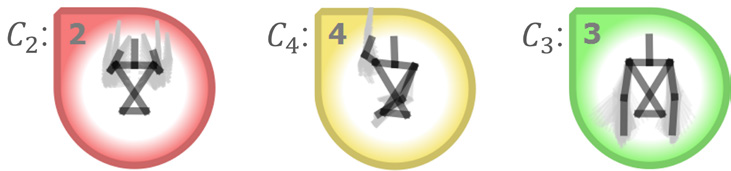
\includegraphics[width=.8\linewidth]{clus-MotionFlow}
	\caption{Visual representation of human pose clusters. \is{Jang2016}}
	\label{fig:lr-MotionFlow}
\end{figure}

MotionFlow uses a force-directed graph of clusters to illustrate their relationship with node distance mapping to the similarity of pose clusters and edges indicating the directed transition between two clusters. Edges are color coded to represent the transition frequency. A user is allowed to interactively change the number of clusters, enabling exploration of the dataset. However, the re-clustering process may change all existing clusters and make it difficult for the user to keep track. To address this issue, MotionFlow allows the user to select the clusters to be locked or unchanged during the re-clustering process. He or she is also able to interactively merge or split clusters according to his or her own assessment.

To achieve the same objective of gaining an overall understanding of human motion tracking data, MotionExplorer~\cite{Bernard2013} applies a different cluster analysis method -- hierarchical clustering~\cite{Han2011} -- which seeks to build a hierarchy of clusters. MotionExplorer takes a divisive approach considering all data items starting within the same cluster and splitting them until a termination condition is met. One of the important decisions in this clustering technique is to determine which cluster to split next. The user is allowed to choose among several splitting strategies such as \emph{maximum standard deviation} to split the most varied cluster first and \emph{highest number of elements} to split the largest cluster first. The hierarchy is visualized as a dendrogram as in \autoref{fig:lr-MotionExplorer}. Clusters are obtained by cutting the dendrogram at the desired vertical level: each connected branch forms a cluster. The vertical axis of the dendrogram can encode different variables depending on the splitting strategy. In \autoref{fig:lr-MotionExplorer}, it shows the standard deviation of each cluster and the user is allowed to slide the cutting value to adjust the resulting clusters.

\begin{figure}[!htb]
	\centering
	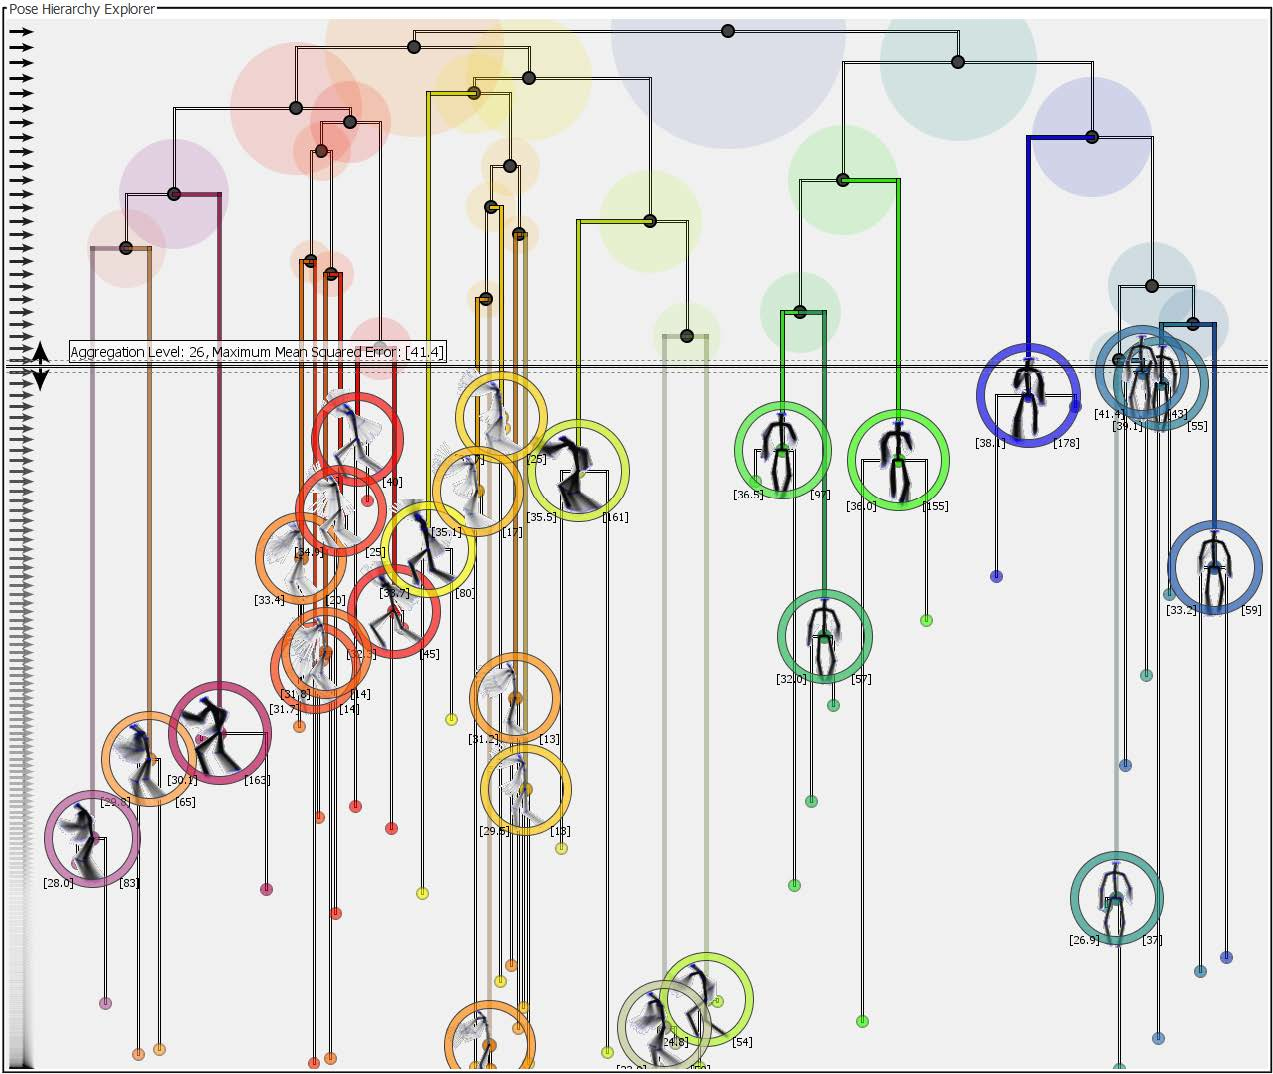
\includegraphics[width=\linewidth]{clus-MotionExplorer}
	\caption{A divisive hierarchical clustering of human poses visualized as a dendrogram. \is{Bernard2013}}
	\label{fig:lr-MotionExplorer}
\end{figure}

A different approach in hierarchical clustering is bottom-up or agglomerative clustering. The process starts with singleton clusters before merging the most similar clusters together until a termination condition is met. NewsLab~\cite{Ghoniem2007} applies such an approach in analysis of large scale broadcast news video collections. It builds a hierarchy of clusters over all keywords extracted from available video captions based on their co-occurrences in the news stories. Therefore, strongly correlated keywords are grouped into the same clusters whereas loosely related keywords are separate in different clusters. Each cluster is visualized as a stream showing the evolution of the keywords within the cluster over time with closely related clusters placed close to each other to allow navigation to different depths of the cluster hierarchy (\autoref{fig:lr-NewsLab}).

\begin{figure}[!htb]
	\centering
	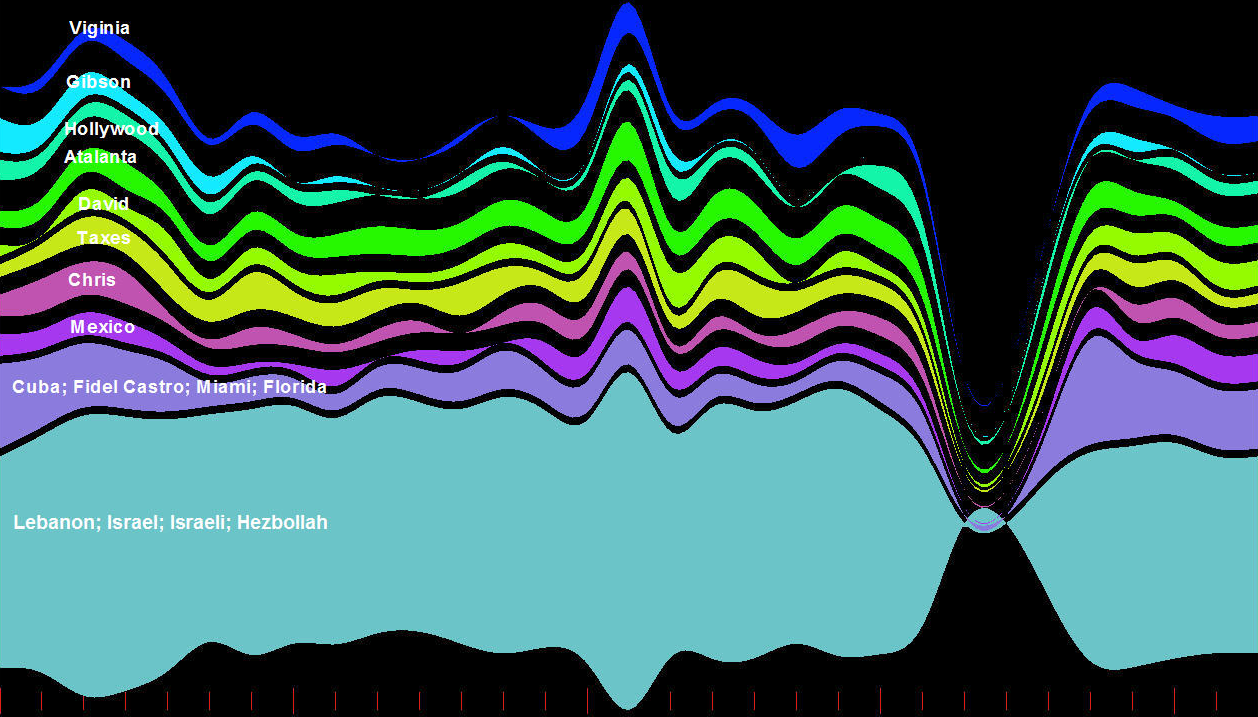
\includegraphics[width=\linewidth]{clus-NewsLab}
	\caption{An agglomerative hierarchical clustering of video captions visualized as streams. \is{Ghoniem2007}}
	\label{fig:lr-NewsLab}
\end{figure}

Understanding people movement patterns in both space and time plays an important role in urban planing. Analyzing and presenting large and complex datasets that contain a number of people in different places and their movement between those places over time are challenging. Mobility Graphs~\cite{Landesberger2016} applies cluster analysis to simplify the data in both spatial and temporal dimensions to gain an overall understanding of the datasets. First, it aggregates places using a density-based clustering technique that considers both the density of places and their flow magnitudes so that close and highly connected can be grouped together. Second, temporal aggregation groups the time steps by the similarity of those simplified places using a k-means clustering technique. \autoref{fig:lr-MobilityGraphs} shows 7 temporal clusters of simplified places. The clusters are color coded with a calendar view to reveal temporal patterns over a week. In each cluster, a node shows an aggregated place with size corresponding to the total number of people in all individual places and arrow widths representing the number of people moving between two aggregated places.

\begin{figure}[!htb]
	\centering
	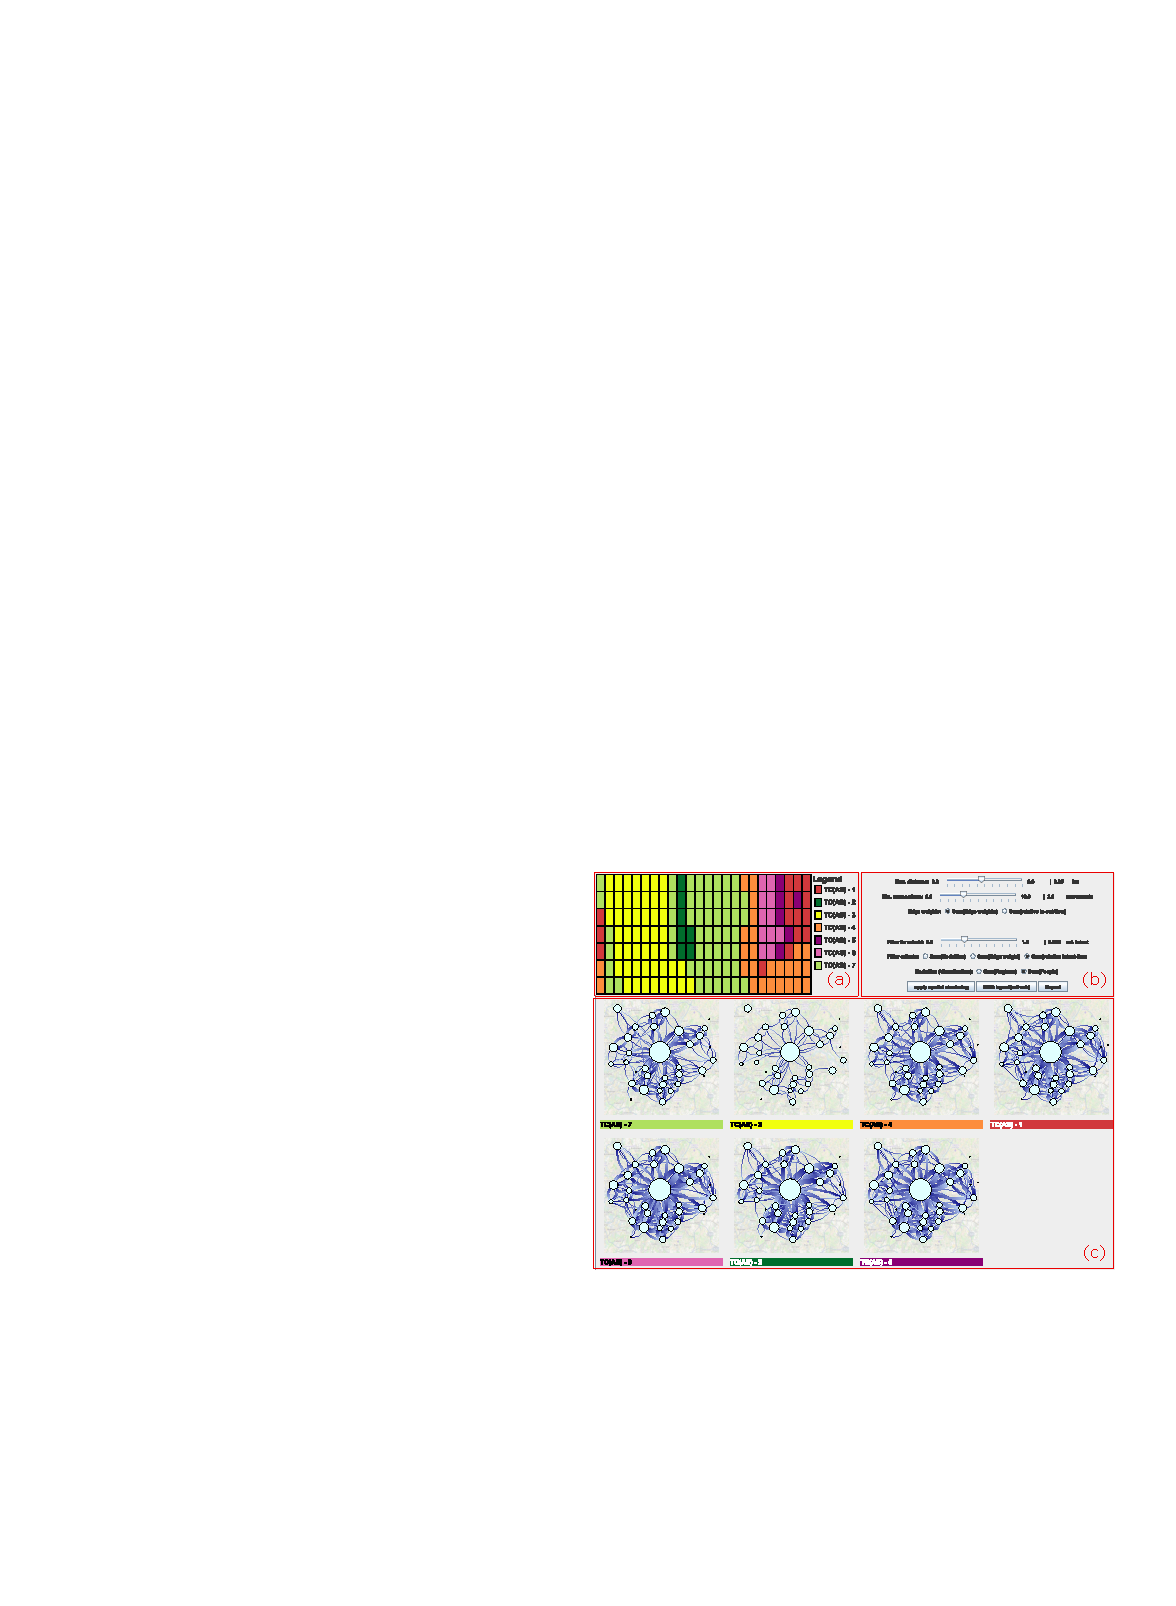
\includegraphics[width=\linewidth]{clus-MobilityGraphs}
	\caption{Temporal clusters of simplified places. \is{Landesberger2016}}
	\label{fig:lr-MobilityGraphs}
\end{figure}

\subsubsection{Classification}
\paragraph{Overview}
Classification predicts the value of a categorical (discrete or nominal) attribute based on the values of other attributes. It builds a model (or \emph{classifier}) based on a labeled training dataset (i.e., \emph{supervised learning}) and applies it in labeling new data~\cite{Han2011}. The model needs to not only identify the labels in the training dataset well but also be general enough to predict the labels of new data correctly. One common and intuitive classification algorithm is decision tree induction~\cite{Quinlan1986}. Each non-leaf node represents a ``test'' on an attribute, which splits the node to multiple branches, each for an outcome of the test. Each leaf node is associated with a class label and is the result of a sequence of tests starting from the root node.

The importance of building a decision tree is choosing which attribute to split at each node. Intuitively, we should choose attributes that can divide nodes into ``pure'' child nodes so that all data items in a child node belong to a single class and no further splits is needed. For example, in a binary classification, consider a training dataset with 10 records, 5 labeled ``true'' and 5 labeled ``false''. Attribute $A1$ splits the set to two subsets: (5 ``true'', 0 ``false'') and (0 ``true'', 5 ``false''). Attribute $A2$ splits the set to (3 ``true'', 2 ``false'') and (2 ``true'', 3 ``false''). The subsets split by $A1$ is ``purer'' than the one by $A2$ because they do not contain a mix of ``true'' and ``false''. To achieve this purity, several attribute measurements have been proposed such as \emph{information gain} and \emph{gini index}~\cite{Tan2006}. More detailed analysis of these measurements and other classification algorithms are out of the scope of this thesis and can be found in data mining textbooks~\cite{Tan2006,Han2011}.

\paragraph{Application Examples}
Exploring a large image collection, such as the set of images available on the Internet, is challenging. Besides the low-level visual features, the semantic contents of images are also effective in searching for relevant ones. Image classification techniques can be used to extract such semantic contents. For example, Fan~et~al.~\cite{Fan2004} detect salient objects in images and associate them with predefined semantic contents according to their perceptual properties. Similar contents are then grouped into a higher level semantic concept; for instance, ``sand field'', ``sea water'' and ``boat'' salient objects construct the concept of ``sea world''. Visualization can help make the output of classification algorithms more interpretable and interactive. To provide an overview of an image collection, Yang~et~al.~\cite{Yang2006} shows the extracted semantic contents, with each as a glyph, in a 2D display so that related contents are located close together using a multidimensional dimension scaling method~\cite{Borg2005}. Similarly, images are also displayed based on their similarity as in \autoref{fig:lr-SIBa}. Zooming and panning are provided to make the visualization more scalable. When an image is selected, the visualization can be switched to a \emph{rainfall} mode, in which the selected image is shown at the bottom and related images are stacked above it based on their similarity with the selected one (\autoref{fig:lr-SIBb}). Users are allowed to reassign the contents computed for each image; however, the model does not take into account the changes to improve its accuracy when classifying new images.

\begin{figure}[!htb]
\centering
\subcaptionbox{Multidimensional dimension scaling view of images.\label{fig:lr-SIBa}}{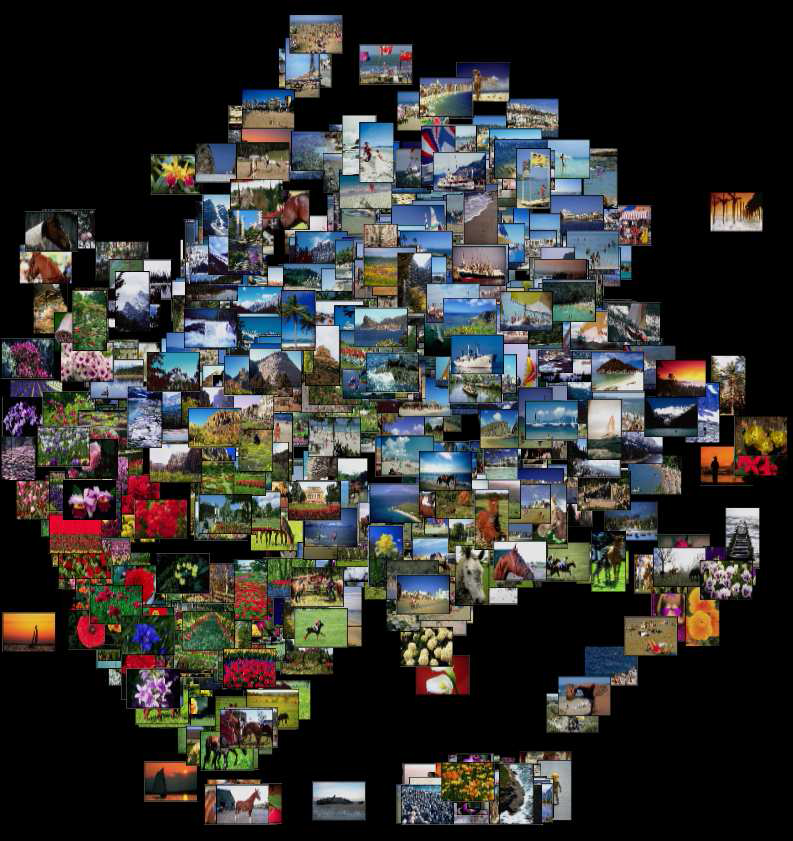
\includegraphics[height=.5\columnwidth]{clas-SIBa}} 
\hfill
\subcaptionbox{Rainfall view of a selected image with highly related images at the bottom.\label{fig:lr-SIBb}}{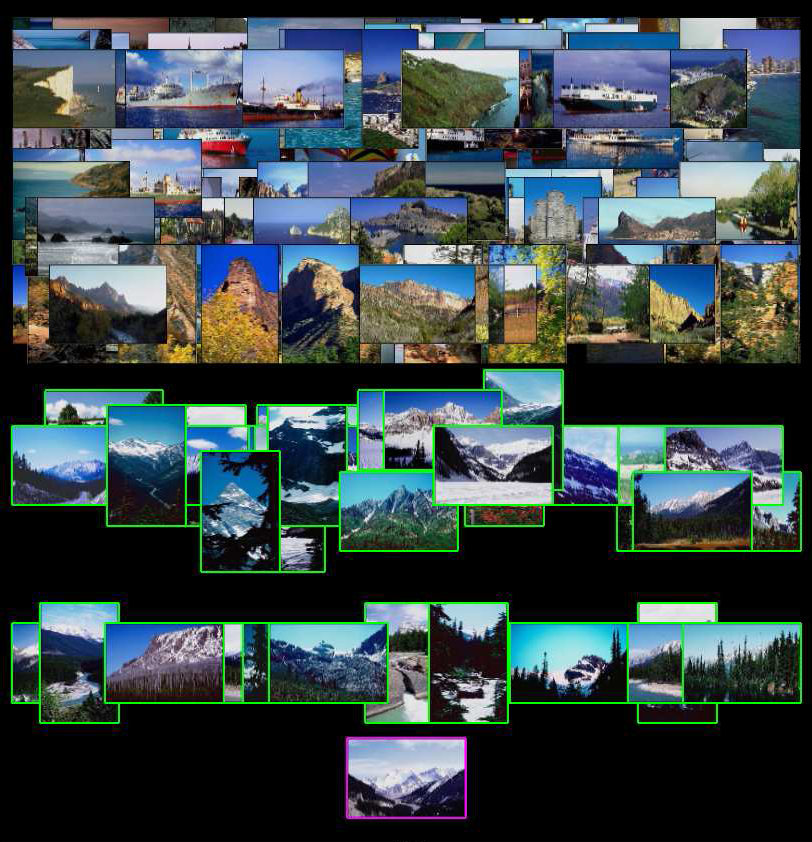
\includegraphics[height=.5\columnwidth]{clas-SIBb}} 
\label{fig:lr-SIB}
\caption{Semantic image browser. \is{Yang2006}}
\end{figure}

In a binary classification, the classifier output is either \emph{positive} or \emph{negative}. Two types of error can happen include \emph{false positive} (classified as positive but the actual class is negative) and \emph{false negative} (classified as negative but the actual class is positive). Depending on a domain, the costs of these error types might be considerably different. For example, wrong prediction of a healthy patient with a cancer has a much lower impact than missing a patient with a real cancer. Migut and Worring~\cite{Migut2010} allow users to adjust the trade-off between these two error types through the visualization of the classification model. Typically, a receiver operating characteristic curve~\cite{Fawcett2006} is used to illustrate the performance of a binary classifier as its discrimination threshold is varied. The curve is composed from a set of true positive rate and false positive rate pairs at various threshold values. Migut and Worring~\cite{Migut2010} replace the true positive rate with the false negative rate (\autoref{fig:lr-Migut1}) because their focus is comparing trade-off between the two error rates. Numerical data is visualized in a scatter plot with the decision boundary separating a 2D plane into two regions, each for a class (\autoref{fig:lr-Migut2}). For each data point, color shows the original class and size indicates the accuracy of the classified class. The current classification setting is shown as a red point on the performance curve, and the user is allowed to move that point along the curve to change the false positive and false negative rates. The classification reruns with the new threshold and rates and updates on the data scatter plot.

\begin{figure}[!htb]
\centering
\subcaptionbox{Performance curve of the classification model with horizontal axis showing the false positive rate and vertical axis showing the false negative rate. rates.\label{fig:lr-Migut1}}[\columnwidth]{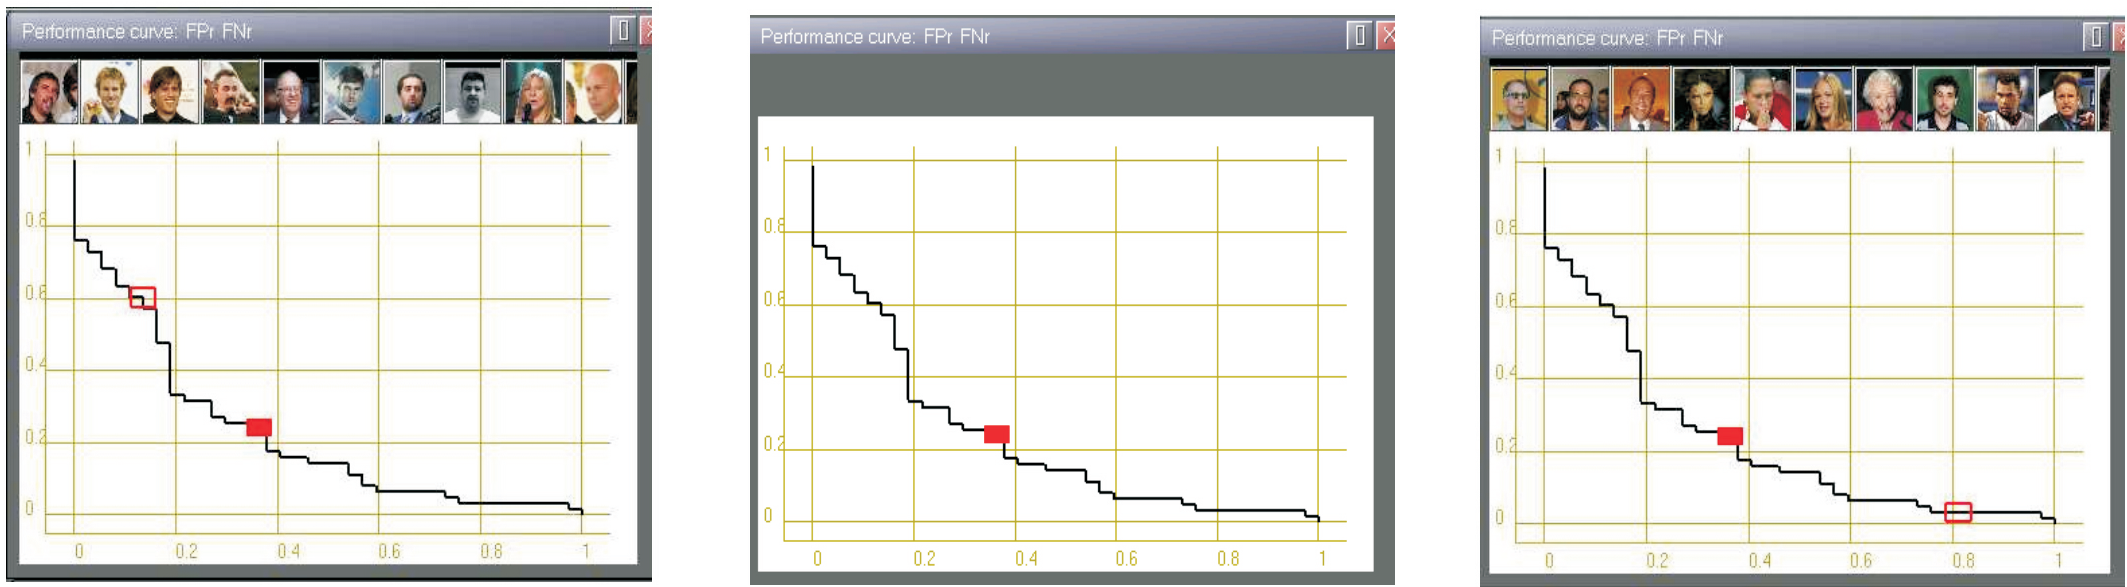
\includegraphics[width=\columnwidth]{clas-Migut1}} 
\\
\subcaptionbox{Data with color indicating original class and size showing classification accuracy.\label{fig:lr-Migut2}}[\columnwidth]{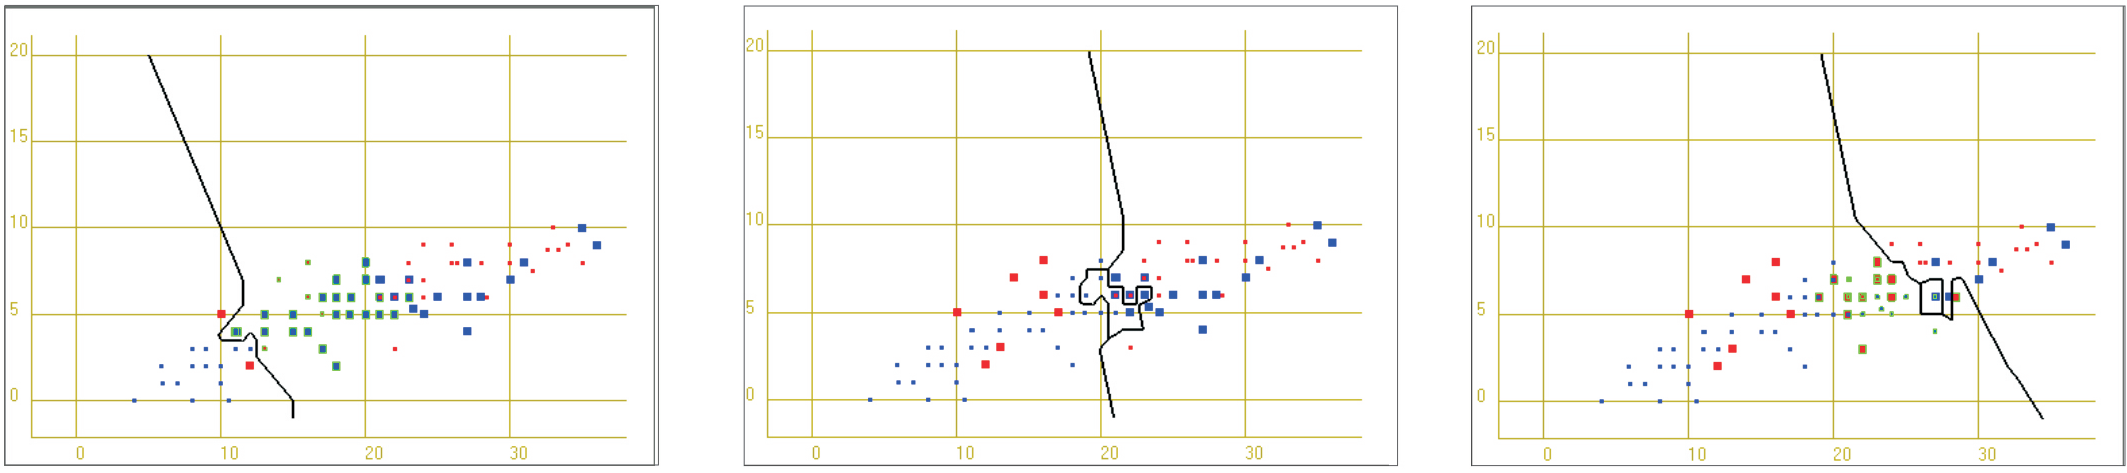
\includegraphics[width=\columnwidth]{clas-Migut2}}
\caption{Visualization and interaction of a classification model. Figure in the middle shows the initial state of the system, with initial operating point on the performance curve and corresponding data scatter plot. Figure on the left shows the state of the system when an expert manipulates the operating point to include more false negatives and on the right to include more false positives. \is{Migut2010}}
\end{figure}

Classification requires training data; however, it can be time-consuming and laborious to produce such a dataset. ScatterBlogs2 includes an interactive classifier that speed up the training data labeling and classifier construction before applying it in real-time monitoring messages of interest~\cite{Bosch2013}. First, the user can search for relevant messages using a standard keyword query. The system then highlights non-trivial terms that frequently co-occur with the original keywords. The result set of highly relevant messages can be used as \emph{positive} samples, whereas some arbitrary messages not returned in the result set can be used as \emph{negative} ones. After creating an initial classifier, the user can inspect messages to correct and update the classifier through the message visualization. Messages are shown in a map as a colored glyph with color hue indicating class and brightness showing classification confidence (\autoref{fig:lr-ScatterBlogs2}). Messages can be filtered by confidence, allowing the user to focus on ones with less certainty, which need human expert to verify. To further speed up the classifier creation, ScatterBlogs2 offers self-training, a technique that iteratively uses messages classified with the highest confidence as labeled data. 

\begin{figure}[!htb]
	\centering
	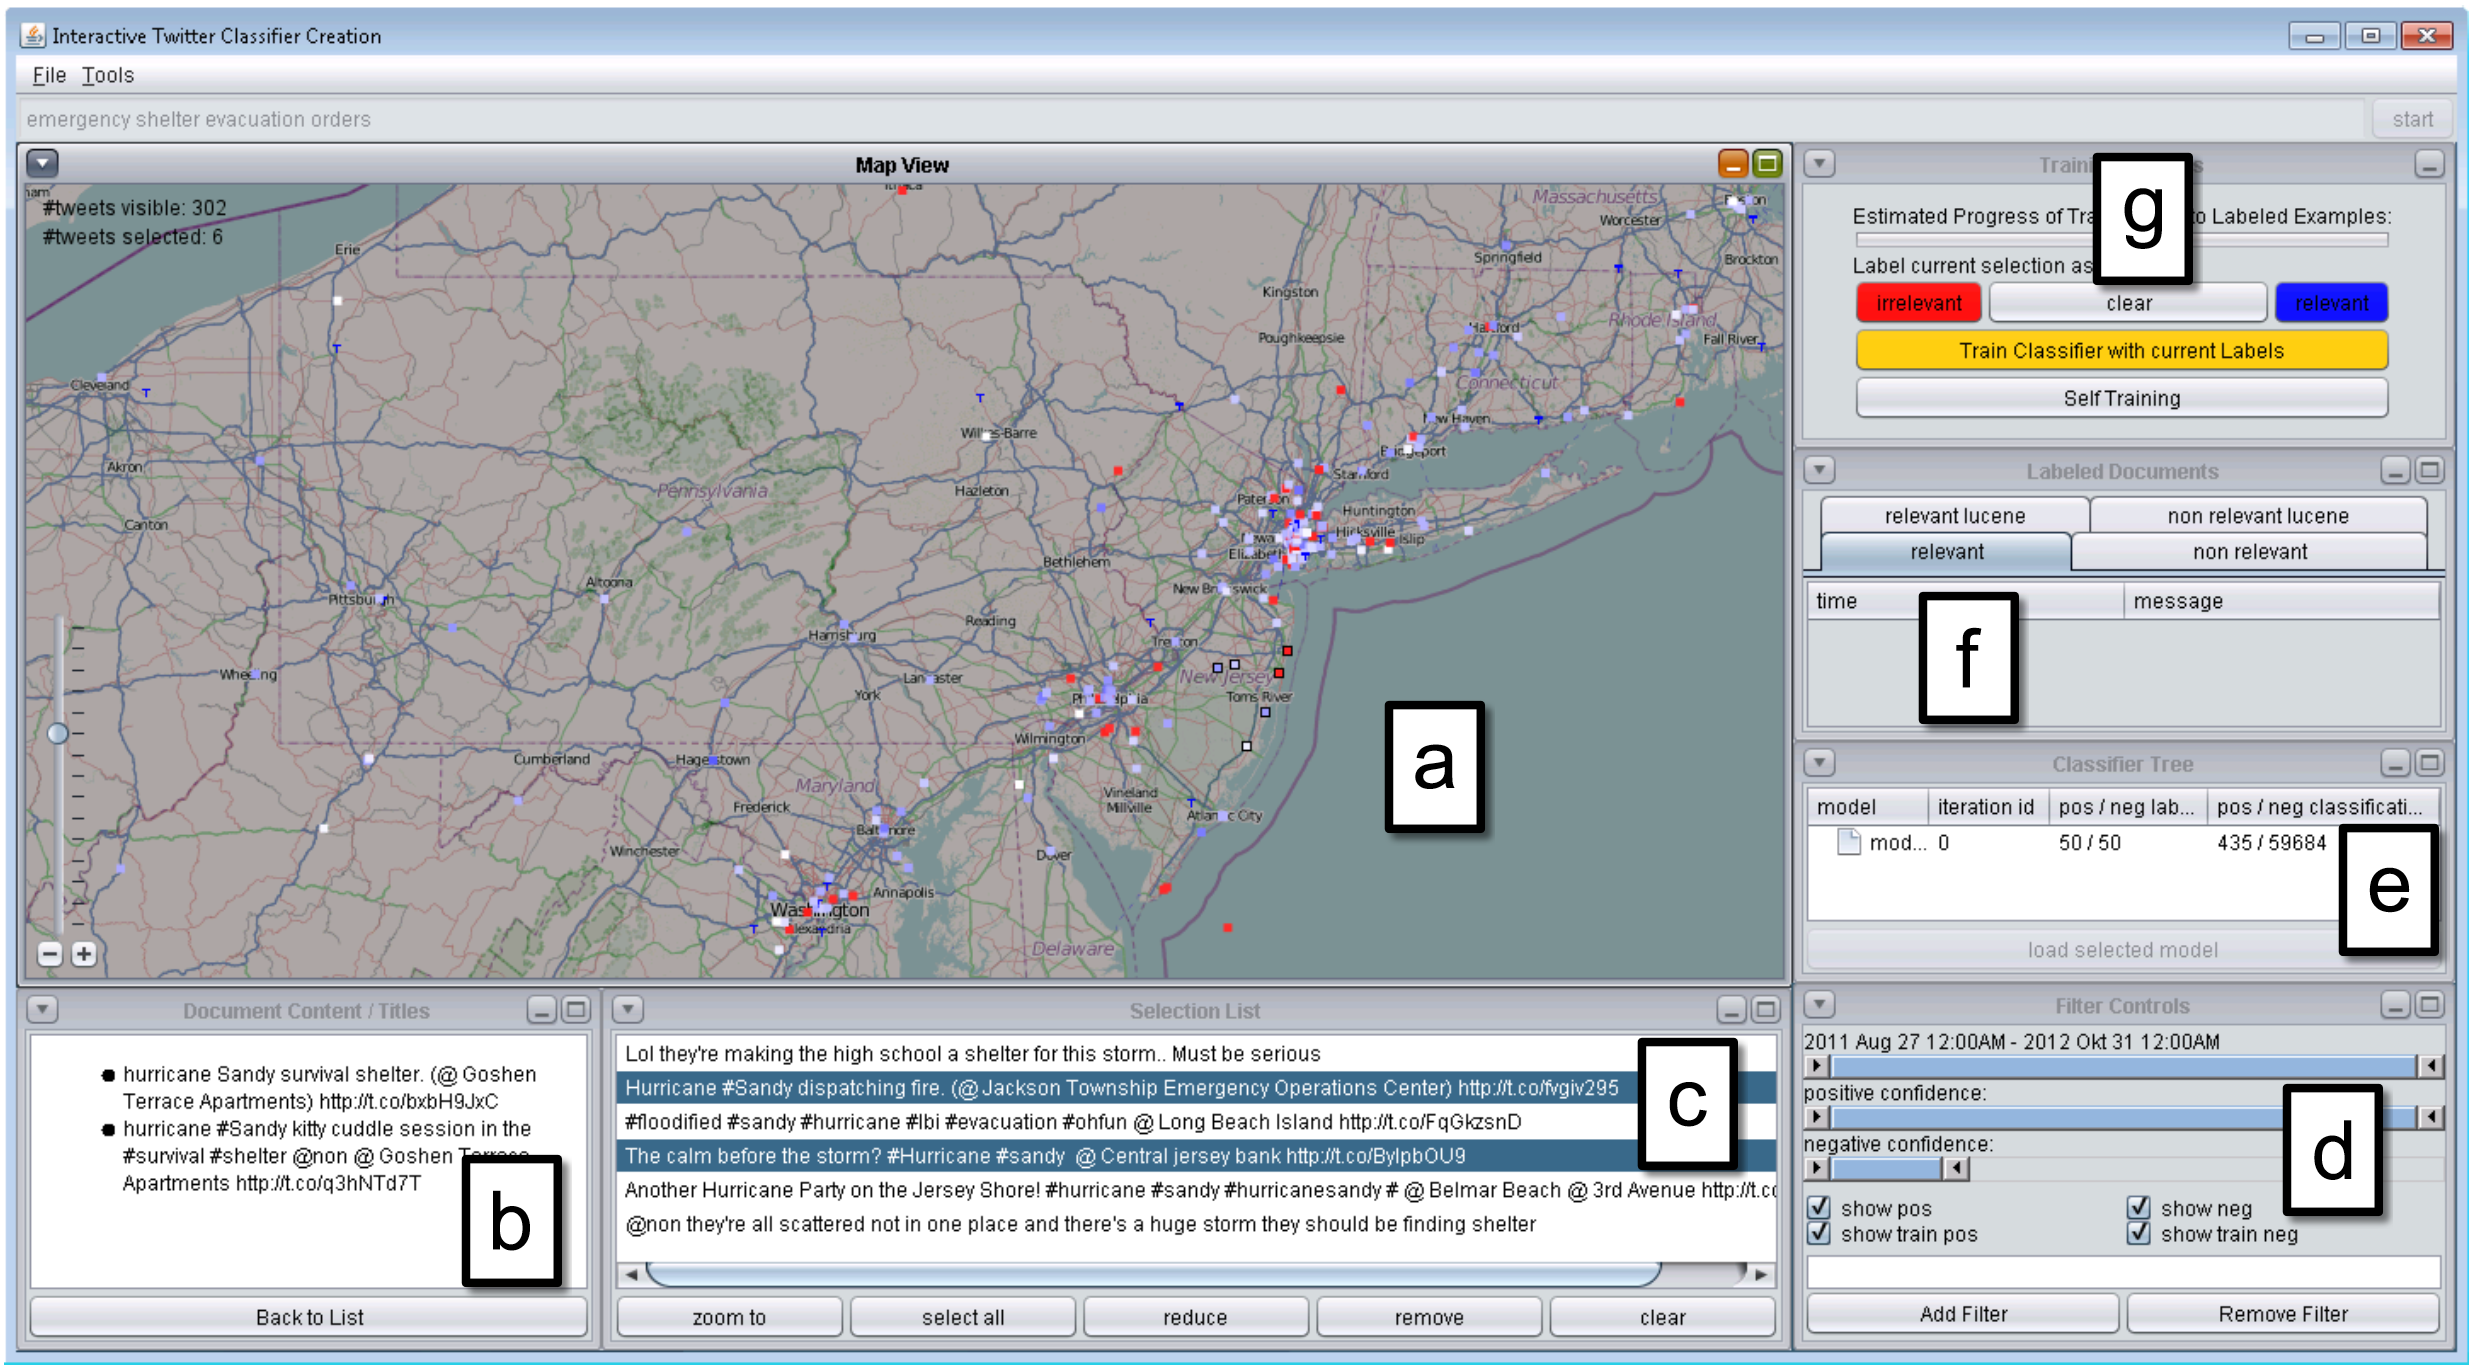
\includegraphics[width=\linewidth]{clas-ScatterBlogs2}
	\caption{The classifier creation environment of ScatterBlogs2. \is{Bosch2013}}
	\label{fig:lr-ScatterBlogs2}
\end{figure}

An essential step in classification of high dimensional datasets is feature selection, which selects a subset of relevant features for use in model construction without much loss of information. This step also simplifies the model and reduces training time. INFUSE~\cite{Krause2014} supports users to explore the predictive power of features in their models. The system allows comparison of features across four feature selection algorithms. Each feature is shown as a circle glyph divided into four equal quadrants, each for an algorithm (\autoref{fig:lr-INFUSE}). A quadrant is further split into 10 slices, each for a cross-validation fold (or random subset of data) to ensure the result  robust. The length of a slice indicates the rank of that feature using a given algorithm. Therefore a glyph can show how its feature performs in different algorithms. To have an overview of all features, INFUSE shows multiple glyphs in either a sequential layout or a scatter plot, where different options can be used for axes such as average rank of a feature or a more sophisticated importance measurement. It also allows users to explore four classification algorithms by showing the score of all 16 combination of feature selection and classification algorithms. More importantly, users are allowed to build their own model by selecting features besides the ones produced by the four given algorithms. The custom feature set is then included in the classification score comparison.

\begin{figure}[!htb]
	\centering
	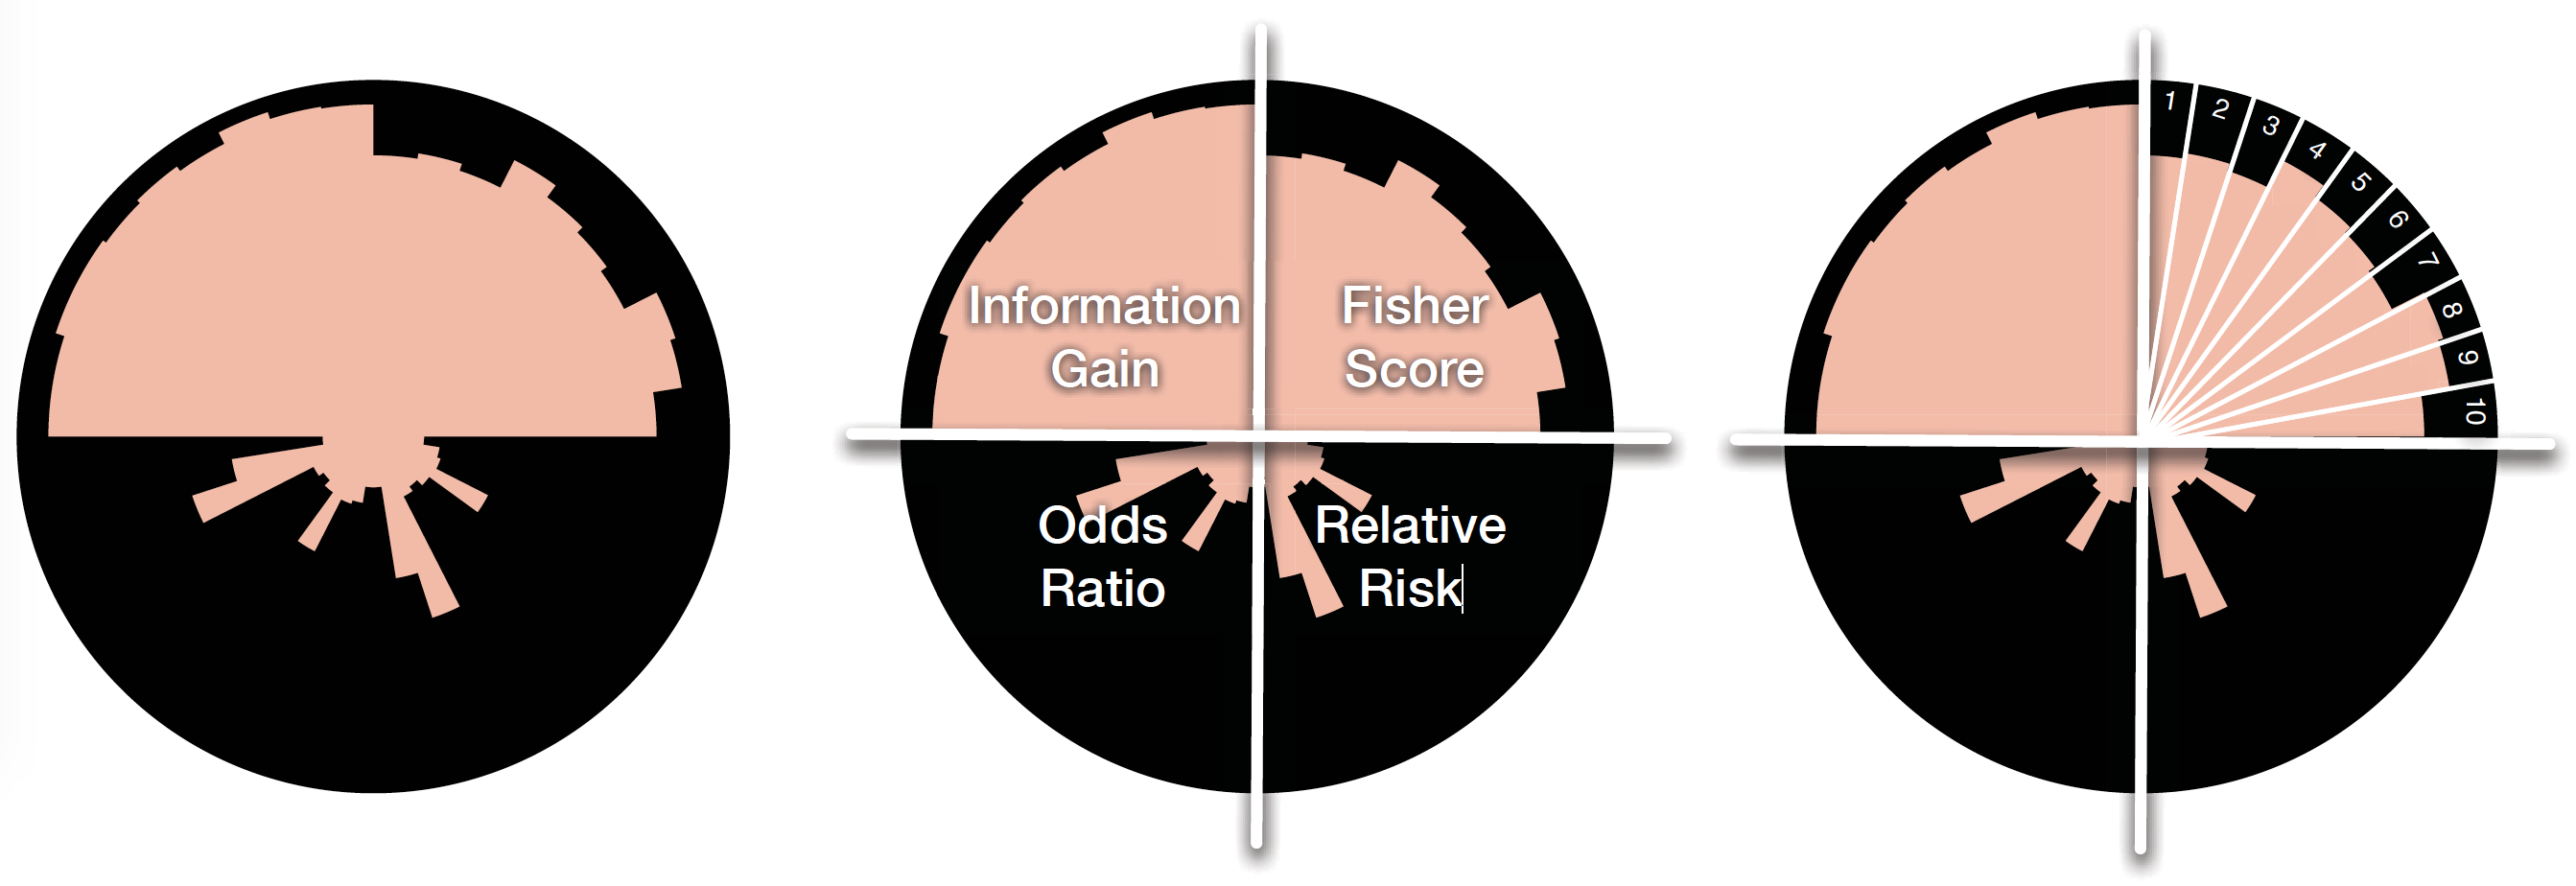
\includegraphics[width=\linewidth]{clas-INFUSE}
	\caption{The feature glyph in INFUSE. \is{Krause2014}}
	\label{fig:lr-INFUSE}
\end{figure}

\subsection{Evaluation Methods}
A visualization, no matter how novel and interesting it is, needs to be evaluated to check whether it meets the design goals and supports the target users to complete the intended tasks. Evaluation has been a research topic in visualization when the field becomes more matured~\cite{Plaisant2004}. Excellent reviews of visualization evaluation with different perspectives include evaluation techniques~\cite{Carpendale2008}, scenarios~\cite{Lam2012} and design process~\cite{Munroe2009}.

In this section, we review the evaluation techniques based on the visualization design model by Munzner~\cite{Munroe2009}, helping address different concerns separately. The four levels include: explain the tasks and available data in the vocabulary of the problem domain, abstract them into domain-independent operations and data types, design visual encoding and interaction techniques to solve the abstract tasks, and develop algorithms to execute these techniques efficiently. Each level has its own \emph{threats} to validity and methods to address them. Two types of methods are distinguished: \emph{immediate} approaches can be done before inner levels are implemented, whereas \emph{downstream} approaches requires all inner levels are completed. The threats and evaluation methods are summarized in \autoref{fig:lr-nested-model}.

\begin{figure}[!htb]
	\centering
	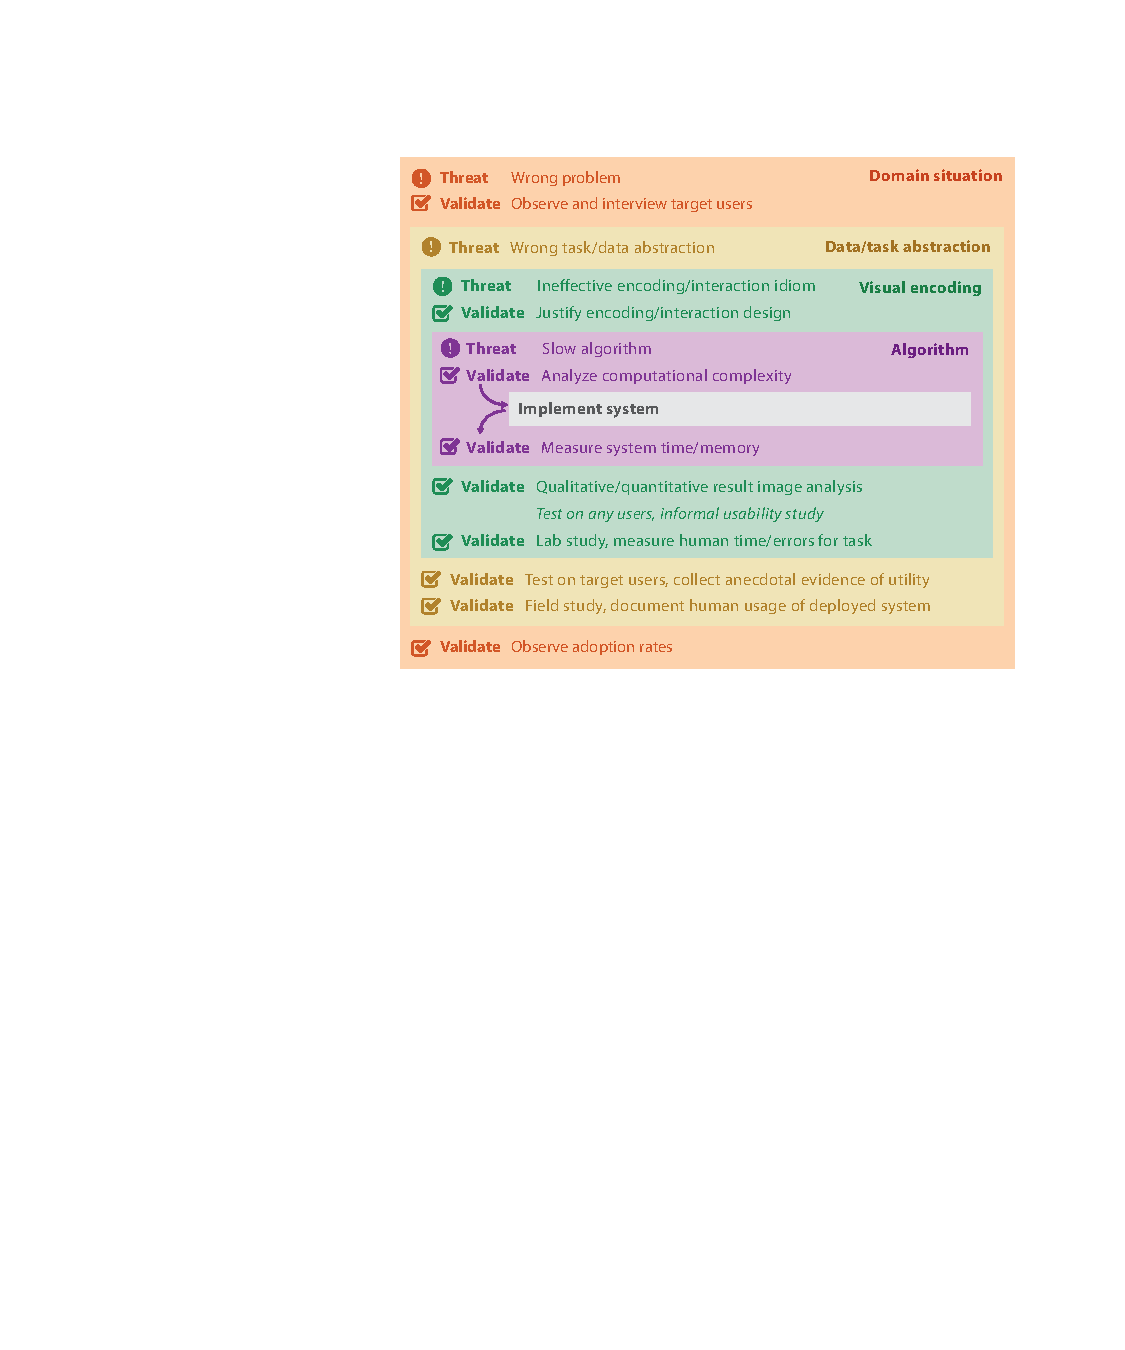
\includegraphics{nested-model}
	\caption{Threats and validation at each of the four nested levels of visualization design. \is{Munzner2014}}
	\label{fig:lr-nested-model}
\end{figure}

\subsubsection{Domain Problem and Data Characterization}
The domain problem of target users is investigated to see if visualization is a potential solution. The primary threat is that the problem is mischaracterized: the users do not really suffer from the identified problem. An immediate form of validation is \emph{field study}~\cite{Carpendale2008}, where the investigator observes how target users act in real-world settings in order to learn and verify the characterization. Another technique is \emph{contextual inquiry}~\cite{Holtzblatt1993}, which allows the investigator to occasionally interview while the user is engaged in the process. One example is the study by Sedlmair~et~al.~\cite{Sedlmair2008} on current working behavior and environments of analysis and diagnosis experts in the automotive industry.

One downstream form of validation is to report the rate the adoption rate of the tool by the target users. High effort is required to make the visualization solution reliable and deployable in the real-world environment. Examples include a field study of Google's Notebook product~\cite{Russell2008} and 6-week field trial of SparTag.us -- a tagging system for foraging web content~\cite{Hong2008}.

\subsubsection{Operation and Data Type Abstraction}
The threat at this level is the identified data and task abstraction do not solve the characterized problem. Only downstream approaches can be used to validate the abstraction. The deployed system needs to be used by target users completing their routine tasks in real-world environment. The goal of this evaluation is to collect anecdotal evidence that the solution is in fact useful. The observation and interview need to focus on understanding how the tool is used, and how it helps or hinders the users in performing their tasks. An example is a longitudinal field study of LiveRAC system that supports analysis of system management time-series data~\cite{McLachlan2008}.

Evaluating the visualizations for supporting sensemaking can be done at this level, as the \emph{evaluating visual data analysis and reasoning} scenario in the taxonomy by Lam~et~al.~\cite{Lam2012}. Due to the nature of sensemaking, evaluation is often carried out as case studies~\cite{Kang2011} with observation and interview, and followed by qualitative data analysis~\cite{Lazar2010}. Attempts also have been made to quantify the insight or knowledge gained during sensemaking~\cite{Wilson2013}.

\subsubsection{Visual Encoding and Interaction Design}
At the design level, the threat is the chosen design is ineffective at communicating the desired abstraction to the user. One immediate form of validation is to justify every design decision based on known design principles such as the ones discussed in \autoref{sub:lr-design}, or more comprehensive predefined guidelines as in heuristic evaluation~\cite{Zuk2006}. Asking experts to review the design prototype also provides valuable feedback~\cite{Tory2005}.

A common downstream approach is to conduct a controlled experiment comparing the design with other state-of-the-art alternatives~\cite{Xu2012}. A number of participants, depending on the  expected size of the experiment, carry out a number of tasks representing real-world cases. Typically, task completion time and accuracy are measured and analyzed using hypothesis testing methods~\cite{Field2003}. Post-task interviews are often combined to establish deeper understanding about how the visualization is used. If the experiment can be completed online, crowd-sourcing approach using Amazon's Mechanical Turk service can help largely increase the size of participants~\cite{Heer2010a}. Another downstream approach is the measurement of common aesthetic metrics such as the number of edge crossings and edge bends that have been used in graph visualization~\cite{Sugiyama1981}.

\subsubsection{Algorithm Design}
The primary threat at this level is the algorithm is suboptimal in terms of time or memory performance. In interactive visualization, it is essential to ensure the interaction responsive in real-time. Analyzing the complexity of the algorithm using the standard approaches from the computer science literature~\cite{Cormen2009} is an intermediate form of validation. The complexity can be computed based on the size of dataset or the display screen. Downstream approaches include measuring running time and memory usage for benchmark datasets.

%http://www.cc.gatech.edu/~stasko/papers/vast09-eval.pdf
%https://www.purdue.edu/discoverypark/vaccine/assets/pdfs/publications/pdf/Beyond%20Usability.pdf
%http://www.cc.gatech.edu/~stasko/7450/Papers/fekete08.pdf
%https://www.cs.ubc.ca/~tmm/courses/cpsc533c-05-fall/readings/vov.pdf
\section{Provenance}
todo: different of data and analytic provenance.Provenance in ordinary context, give examples (food, art)
where?
%must read: very releveant: http://www.cc.gatech.edu/~aendert3/resources/ragan-vast-2015.pdf
\subsection{Data Provenance}
Data provenance research has been taken in different fields, notably scientific workflows and databases. Scientific experiments may consist of thousands of steps, with each step involving distributed data sources and computational data models~\cite{Gil2007}. Workflows have been used to facilitate the assembly, automation and management of such experiments. Notable scientific workflow systems with provenance enabled include Tarvena~\cite{Zhao2008}, Kepler~\cite{Bowers2006} and VisTrails~\cite{Bavoil2005}. Provenance plays an important role in scientific workflows, aiming to support data interpretation, reproduction of experiment results, troubleshooting and optimization~\cite{Miles2007}. The provenance of long and complex workflows is huge, thus pose challenges in storing, querying, and making sense of such data~\cite{Davidson2007}.

Curated databases are populated and updated with a great deal of human effort, typically published on the web~\cite{Buneman2008}. A well-known example is Wikipedia -- a free Internet encyclopedia that allows its users to edit almost any article accessible. Each record in these databases, such as a Wikipedia article, may be edited by many users and referred to other internal and external sources. This produces problems in attribution and provenance: who edited what at when. Research in database provenance can be characterized into a why-where-how framework~\cite{Cheney2007}. \emph{Why}-provenance focuses on the lineage of the output: for each tuple $t$ in the output, the lineage of $t$ is a set of tuples in the input data that helps produce $t$~\cite{Cui2000}. \emph{How}-provenance concerns how the output tuple $t$ is derived from the query~\cite{Green2007}. Finally, \emph{where}-provenance describes specific locations, or cells in relational databases, of the input data that contribute to the query output~\cite{Buneman2001}. To compute these types of provenance, two general approaches have been introduced~\cite{Buneman2008}. An \emph{eager} approach adjusts the query to pass the extra provenance information to the output. Whereas, a \emph{lazy} approach computes provenance on demand.

Data provenance research in scientific workflows and databases has mainly focused on closed systems, which have full access to the data and its provenance. Modern applications with service-oriented~\cite{Papazoglou2007} and cloud-computing~\cite{Buyya2009} architectures bring challenges in tracking and exchanging provenance information across systems. The \emph{Open Provenance Model} is designed to address these challenges~\cite{Moreau2011}. It also supports a digital representation of provenance for any ``thing'', whether produced by computer systems or not. Three types of objects are defined in the model for building this representation. An \emph{artifact} is a state that can be a digital or physical object. A \emph{process} is a series of actions performed on or caused by artifacts, and resulting in new artifacts. An \emph{agent} acts as a catalyst of a process, managing its execution. Different types of causal relationships can be added between these nodes, forming a \emph{provenance graph} as shown in \autoref{fig:lr-provenance-graph}.

\begin{figure}[!htb]
	\centering
	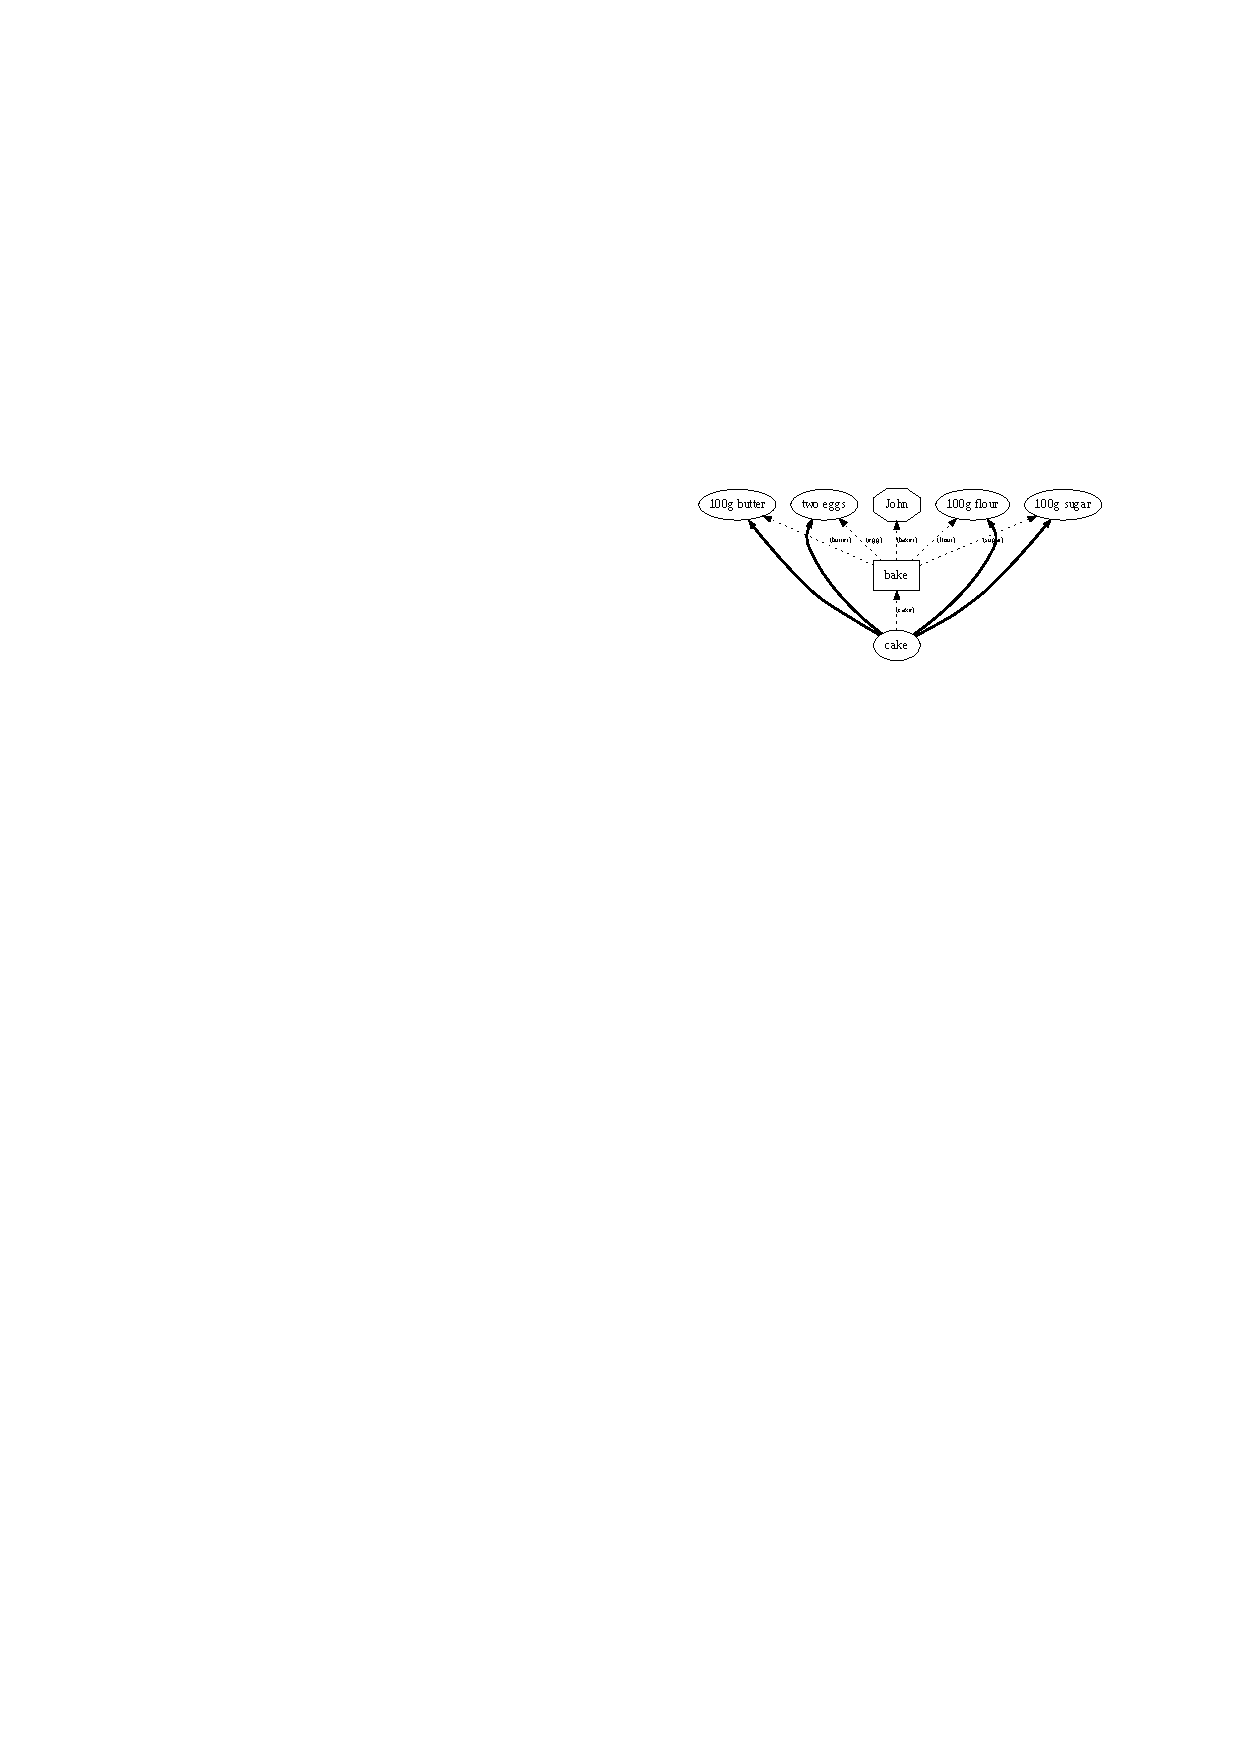
\includegraphics[width=\linewidth]{provenance-graph}
	\caption{A provenance graph for ``cake baking'' using the Open Provenance Model. The cake (artifact) was baked (the process) by John (the agent) using ingredients including butter, eggs, flour and sugar (artifacts). \is{Moreau2011}}
	\label{fig:lr-provenance-graph}
\end{figure}

The Open Provenance Model is general and can be extended in both the structure and vocabulary to represent domain-specific problems. ProveML~\cite{Walker2013} is an extension of this model for recording the provenance of data, analytical process and interpretations in human terrain visual analytics.

\subsection{Analytic Provenance}
Definition from ~\cite{North2011}, our agenda~\cite{Xu2015}

\subsubsection{Model}
Modeling of analytic provenance: 4-level model by Gotz and Zhou and other vis task/action taxonomies such as classic Shneiderman's task by data type~\cite{Shneiderman1996}, Amar's low-level~\cite{Amar2005}, Amar's high-level~\cite{Amar2004}, more recent Bhemer's typology what-why-how~\cite{Brehmer2013}.

\subsubsection{Capture}
combine previous reviews from the draft survey of analytic provenance, research agenda, and capture in the context of online sensenmaking the last paper
%\section{Visualization of Time-Oriented and Network Data}
\label{sub:lr-time-network}

\subsection{Time-Oriented Data Visualization}
Many visualization techniques have been developed to explore the temporal relationships of data. The book by Aigner~et~al.~\cite{Aigner2011} provides a comprehensive review of this topic. It discusses the characteristics of time and time-oriented data (what), the tasks aimed to support (why), and the visual representations of time and data (how). The book also reviews interaction and analytical supports for such visualizations. In this section, we briefly describe different visual mappings of time (as summarized in \autoref{fig:lr-time}) and recommend readers to Aigner~et~al.~'s book for further detail.

\begin{figure}
	\centering
	\subcaptionbox{Joseph Priestley's Chart of Biography as a horizontal timeline. \is{Priestley1765}
	\label{fig:lr-time-horizontal}}{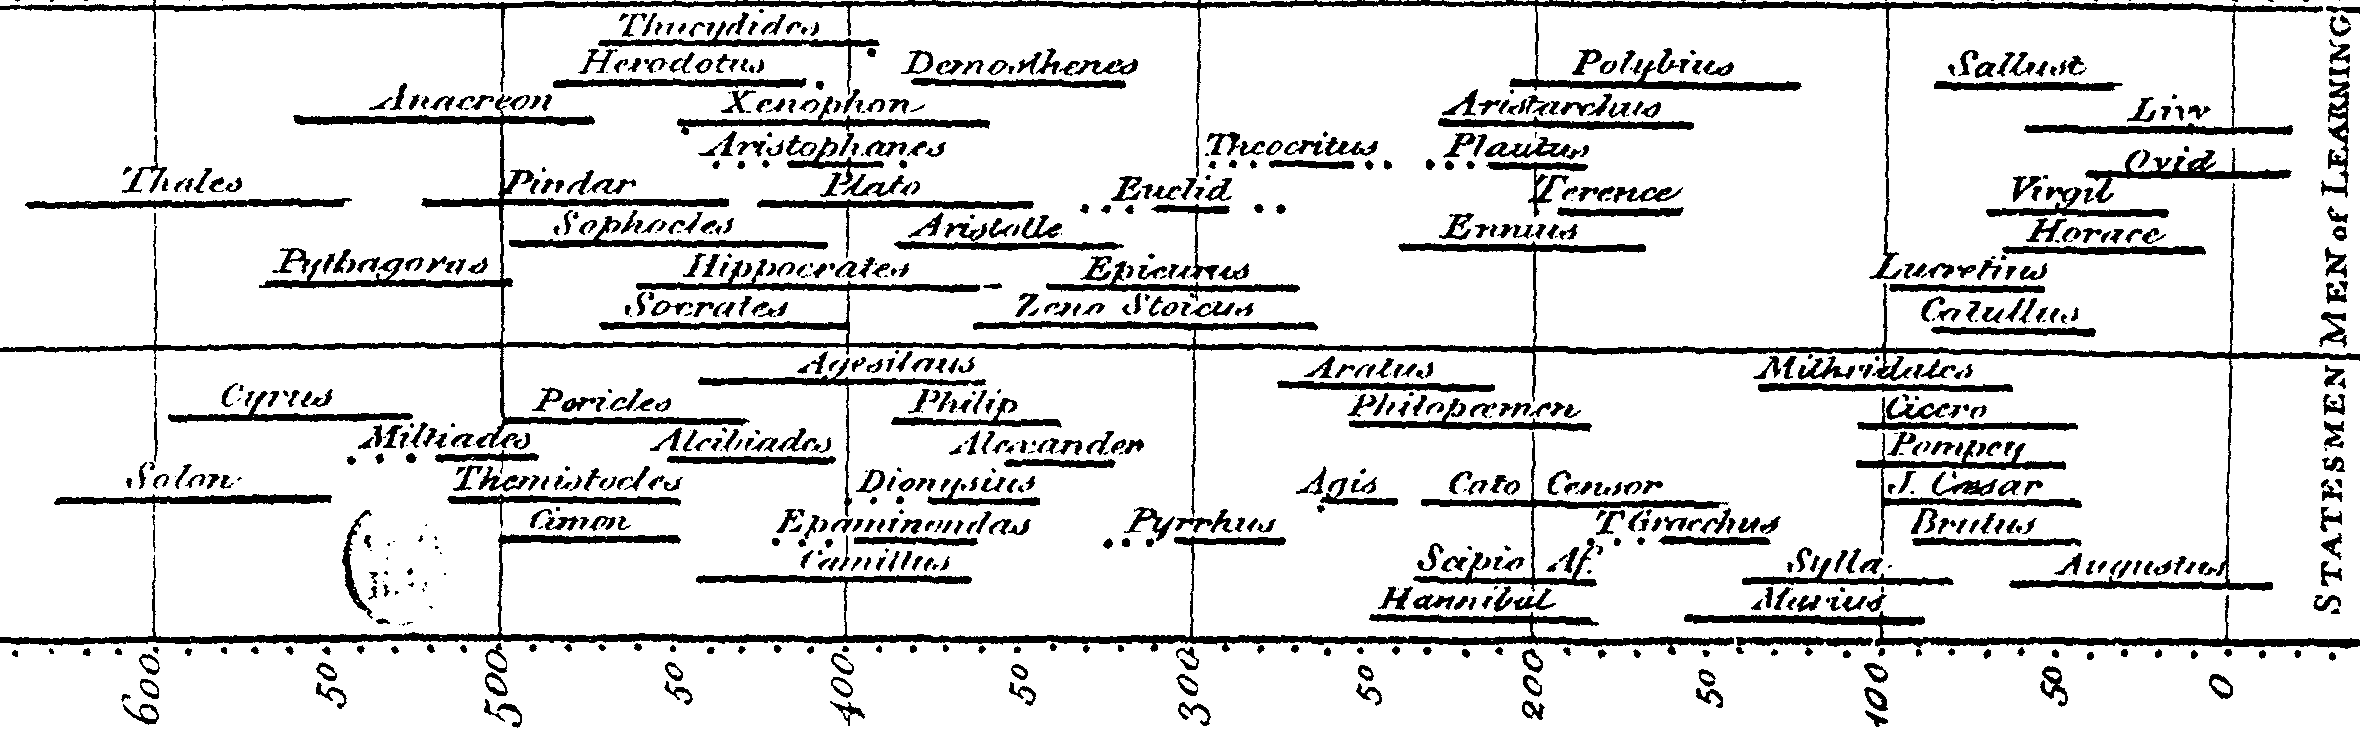
\includegraphics[width=\columnwidth]{biography-chart-crop}}
	\\ \vspace{.5\baselineskip}
	\subcaptionbox{Spiral time axis showing two variables (yellow and red). \is{Weber2001} \label{fig:lr-time-spiral}}[.47\columnwidth]{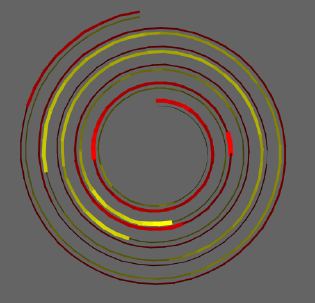
\includegraphics[height=.35\columnwidth]{spiral}}
	\hfill
	\subcaptionbox{Circle time axis showing six variables over ten time steps. \is{Keim2004}
	\label{fig:lr-time-circle}}[.47\columnwidth]{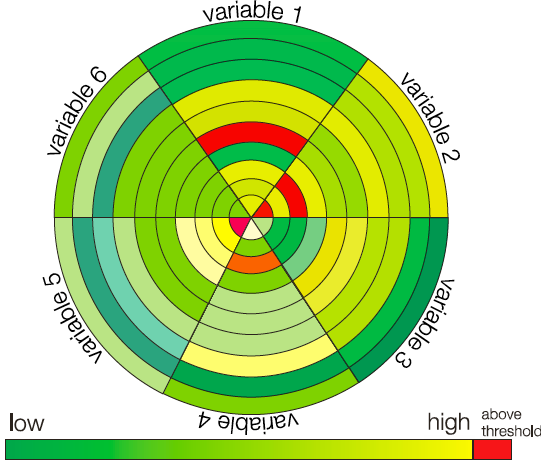
\includegraphics[height=.35\columnwidth]{circle-view}}
	\\ \vspace{.5\baselineskip}
	\subcaptionbox{Calendar visualization of a 6-month data of daily power consumption. \is{VanWijk1999} \label{fig:lr-time-calendar}}{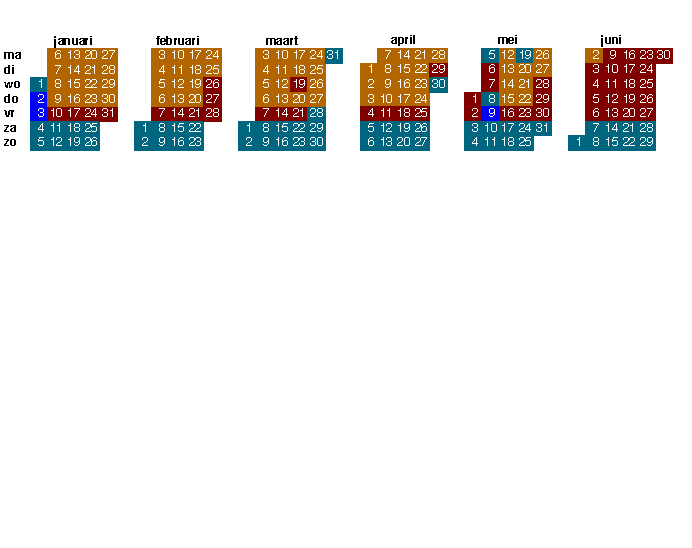
\includegraphics[width=\columnwidth]{calendar-crop}}
	\\ \vspace{.5\baselineskip}
	\subcaptionbox{Small multiples of bar charts showing values from 2001 to 2011. \is{SmallMultiples2014} \label{fig:lr-time-multiples}}{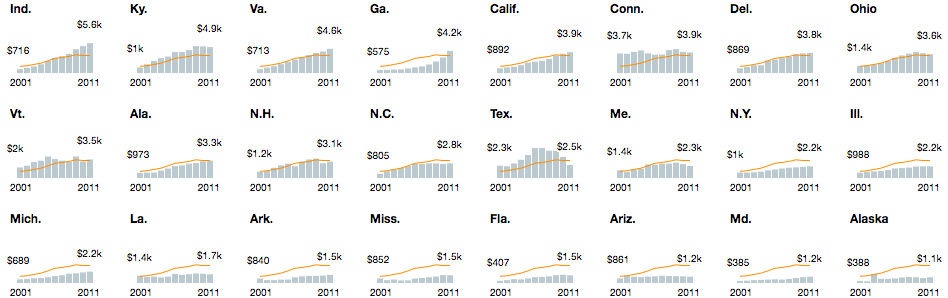
\includegraphics[width=\columnwidth]{small-multiples-crop}}
	\caption{Visual mappings of time.}
	\label{fig:lr-time}
\end{figure}

\subparagraph{Horizontal} Data items are positioned along a horizontal axis as either a point mark for point-based time or a line mark for interval-based time. This is the most common method, and was used in one of the oldest documented timelines -- the \emph{Chart of Biography} by Joseph Priestley~\cite{Priestley1765} back in 1765 -- as shown in \autoref{fig:lr-time-horizontal}. It displays the lifespans of famous people along a horizontal time axis, using a line segment to depict a lifespan, and dots to indicate uncertain values.

\subparagraph{Spiral} Data can be positioned along a spiral axis~\cite{Weber2001}. Color intensity and line thickness are suitable for encoding an additional quantitative variable. Spirals can also be intertwined to show multiple variables. \autoref{fig:lr-time-spiral} shows a spiral graph comparing two variables over time with different color hues.

\subparagraph{Circle} A circle-based approach can be used to visualize time-related multidimensional datasets~\cite{Keim2004}. A circle is split into multiple concentric rings, each for a time step; and is divided into a number of sectors, each representing a variable. \autoref{fig:lr-time-circle} shows such a visualization with six variables.

\subparagraph{Calendar} This method color-codes days in a calendar based on value of a data attribute to reveal patterns at different temporal granularities such as daily, weekly and monthly~\cite{VanWijk1999}. \autoref{fig:lr-time-calendar} visualizes the daily power consumption over a year with color indicating the result of a clustering algorithm.

\subparagraph{Small Multiples}  Miniature data visualization at different time points can be positioned next to each other to facilitate overview and comparison. This method can be applied to all static visualizations because only small screen shots of the visualization for each time step are required. \autoref{fig:lr-time-multiples} shows small multiples of bar charts.

\subparagraph{Animation} This is another time mapping that can be applied to all static visualizations. It relies on human perception in perceiving changes while a visualization smoothly updates from one time step to another~\cite{Gapminder}. Only a few data items should be animated, and they are often highlighted so that users can keep track of the changes.

\paragraph{Summary} Horizontal time axis is a conventional mapping and easy to understand, whereas spiral time axis is good at detecting cyclic patterns. Calendar is another user-friendly representation and can reveal patterns at different granularities. Animation can be an appealing choice for presentation, but it is both slower and less accurate than small multiples in conveying trends over time~\cite{Robertson2008}. In this thesis, \autoref{chap:schemaline} contributes a novel timeline visualization that is inherently designed for sensemaking and based on horizontal time axis mapping. \autoref{chap:timesets} extends the technique to support making sense of complex relationships by showing both temporal and categorical information simultaneously.

\subsection{Network and Tree Data Visualization}
Network visualization is an established research topic with many comprehensive survey papers such as~\cite{Herman2000}. A more recent survey published in 2011 by Landesberger et~al.~\cite{Landesberger2011}. It discusses visual representations of network data together with interaction and analysis techniques. In this section, we briefly describe common methods in visualizing network and tree data (as summarized in \autoref{fig:lr-network}) and recommend readers to aforementioned surveys for further detail.

\begin{figure}[t]
	\centering
	\subcaptionbox{Matrix view with gray cells showing connectivity. \is{Munzner2014} \label{fig:lr-network-nodelink}}[.47\columnwidth]{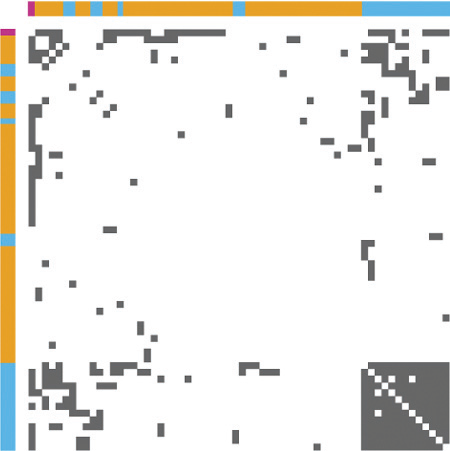
\includegraphics[height=.4\columnwidth]{matrix-2}}
	\hfill
	\subcaptionbox{Force-directed layout with links showing connectivity. \is{Munzner2014} \label{fig:lr-network-matrix}}[.47\columnwidth]{\includegraphics[height=.4\columnwidth]{matrix-3}}
	\\ \vspace{.5\baselineskip}
	\subcaptionbox{Treemap showing the class hierarchy of the Flare visualization toolkit~\cite{Heer2009b}. Area represents class sizes and color represents the top-level classes. \label{fig:lr-network-treemap}}{\includegraphics[width=\columnwidth]{treemap}}
	\caption{Visual representations of network and tree data.}
	\label{fig:lr-network}
\end{figure}

\subparagraph{Node-Link Diagrams}
This is the most common visual encoding for network and tree data, where nodes are represented as \emph{point} marks and links connecting these nodes are represented as \emph{connection} marks. Force-directed layout~\cite{Eades1984} is often used to generate an aesthetically pleasing output based on a simulation of physical forces.  \autoref{fig:lr-network-nodelink} shows an example of a medium-size network.

\subparagraph{Matrix Views}
A network can be represented by an adjacency matrix. Each row and column of the matrix corresponds to a node, and a cell indicates whether the pair of corresponding nodes is connected in the network. Additional information about edges can be encoded to the visual representation of cells using color, shape and size. \autoref{fig:lr-network-matrix} shows an example of matrix view using the same dataset as in \autoref{fig:lr-network-nodelink}.

\subparagraph{Space-Filling Techniques}
Space-filling techniques can only be applied to tree data and uses \emph{containment} marks to represent hierarchical relationship, placing child nodes within their parent node. Treemap~\cite{Shneiderman1992} represents a node as a rectangle, which is recursively subdivided into smaller rectangles, each representing a child of the node. The rectangle size is proportional to a quantitative attribute of its node. \autoref{fig:lr-network-treemap} shows an example of treemap.

\paragraph{Summary}
Node-link diagrams are user-friendly and suitable for small datasets, whereas matrix views are better at large datasets~\cite{Ghoniem2005}. Space-filling techniques produce a compact visualization of tree data and are effective in using size to represent a quantitative attribute. \autoref{chap:sensemap} also uses network data showing pair-wise relationships between provenance data items. Even though it applies an existing tree layout, the research discussed in this section lays the foundation for making suitable design decisions. To address scalability, our tree visualization includes representations for different levels of detail and interactive features such as semantic zooming and panning.

\section{Chapter Summary}
This chapter reviews the background and research related to the problem addressed in this thesis – visualization of analytic provenance for sensemaking. In this section, we briefly preview the relationship between the literature and our designs discussed in subsequent chapters.

Sensemaking support is the ultimate goal of the thesis. We use the Pirolli and Card’s model and the Data–Frame model as the theoretical foundation for sensemaking, and design visualizations to support key parts of those models. These visualizations make use of analytic provenance data captured while the user interacts with the sensemaking system to solve his or her problem. Both manual and automatic capture data are used in this thesis. The visualizations are designed based on a number of well-established design principles and interaction techniques such as Gestalt laws for representing grouping information; brushing \& linking and fluid interaction for coordinating linked views; and semantic zooming with different levels of detail for scalability. Specific design ideas motivated by the literature include using horizontal axis to represent time (from time-oriented visualization) and using node-link diagrams to show pair-wise relations (from network visualization). The designs are validated rigorously using suitable evaluation methods discussed earlier. Design decisions are justified carefully before implementation and case studies with target audience are conducted to explore the effectiveness of the prototypes in supporting sensemaking. For specific design elements, a lab controlled experiment is used (\autoref{chap:timesets}) to compare user performance in simpler tasks such as readability.

The four subsequent chapters will address the four research questions in the same order described in \autoref{intro:questions} based on the knowledge summarized here. The next chapter will address the first research question: designing visualization of timestamped provenance data to explore temporal relationships in sensemaking.